\section{Experiments}
\label{sec:eval}
In this section, we evaluate our techniques along with
The results can be analyzed from four aspects. \textbf{First},  we illustrate the significance of AL in alleviating the labelling burden. \textbf{Second}, we compare the performance using different classifier. \textbf{Third}, we analyze the influence of class number on AL sampling. \textbf{Last but not least}, we try to figure out the correlation between AL outcomes and the dataset feature.


\begin{figure}[th]
	\centering
	%\subfloat[Complaint]{\includegraphics[width=0.2\textwidth]{figs/complaint.eps}}
	\subfloat[Reuters]{\includegraphics[width=0.25\textwidth, height=0.125\textheight]{figs/reuters_dis.eps}}
	\subfloat[TNEWS]{\includegraphics[width=0.25\textwidth, height=0.125\textheight]{figs/tnews_dis.eps}}\newline
	\subfloat[GCS]{\includegraphics[width=0.25\textwidth, height=0.125\textheight]{figs/yanjing_dis.eps}}
    \subfloat[Biomedical]{\includegraphics[width=0.25\textwidth, height=0.125\textheight]{figs/bio_dis.eps}}\newline
    \subfloat[Search Snippets]{\includegraphics[width=0.25\textwidth, height=0.125\textheight]{figs/search_dis.eps}}
    \subfloat[HuffPost]{\includegraphics[width=0.25\textwidth, height=0.125\textheight]{figs/news_dis.eps}}\newline
    \subfloat[Book]{\includegraphics[width=0.25\textwidth, height=0.125\textheight]{figs/book_dis.eps}}
    \subfloat[Emoji]{\includegraphics[width=0.25\textwidth, height=0.125\textheight]{figs/emoji_dis.eps}}
	\caption{Label Distribution of Datasets (Classes (X) vs. Number of 
instances (Y)) 
%\KZ{The y axis should be the number instances for a class. Why is it less than 1}
} 
\label{fig:distribution}
\end{figure}
\begin{table*}[th]
	\scriptsize
	\centering
	\begin{threeparttable}
	\begin{tabular}{ccccccccc}
		\toprule
		& Reuters\tnote{1}  & TNEWS \tnote{2}   & GCS\tnote{3} & Biomedical\tnote{4}  & SearchSnippets\tnote{4}  & HuffPost\tnote{5} & Book\tnote{6} & Emoji\tnote{7} \\ \hline
		Classes       & 66                   & 15         & 141           &20&8       & 41 & 80  & 20   \\
		\#Samples     & 9,442            & 325,285    & 63,792           &20,000&12,340        &200,853&36816&        \\
		Language      & Eng               & Ch         & Ch           & Eng          & Eng    &Eng&Ch& Eng     \\
		Avg Tokens/sample & 6.2              & 13.2        &     6.0     &8.9&18.0    &6.8&6.2&      \\
		Min Tokens/sample & 1 & 1 & 1 &1&1         &0&1&\\
		Max Tokens/sample & 21 & 90 & 115 &39&39    &47&170& \\

		OOV &1,020 &97,154&4,939&4,183&8,156    &7018&4468&34012\\
		Vocabulary& 7,715&144,235&10,591&18,787&29,154     &55442&9722&82742\\
		Desc.         & news title  & news title & customer &paper title&web search transaction &news title&customer&tweets 
   \\ 
	& & &request sentence &  &  &&request sentence &\\
		Label         & topics             & category   & intention                 &topic&domain      &topics&intention&emoji\\
%		Upperbound F1 (fastText) & 0.37       & 0.80          & 0.82       & 0.67      &0.70&0.90&0.93 \\
		\bottomrule              
	\end{tabular}


\begin{tablenotes}
	\item[1] \url{https://archive.ics.uci.edu/ml/datasets/reuters-21578+text+categorization+collection}
	\item[2] \url{https://github.com/ChineseGLUE/ChineseGLUE}
	\item[3] \url{http://Anonimized.for.blind.review}
	\item[4] \url{https://github.com/jacoxu/STC2}
	\item[5] \url{https://www.kaggle.com/rmisra/news-category-dataset}
	\item[6] \url{http://Anonimized.for.blind.review}
	%\item[7] \url{https://competitions.codalab.org/competitions/17344}
	\item[7] \url{https://www.kaggle.com/hariharasudhanas/twitter-emoji-prediction}
\end{tablenotes}
\end{threeparttable}
\caption{Statistics of Datasets.
	Upperbound F1 is macro-average F1 score of fastText trained on all 
	training data. (should be statistics of raw data)}
\label{table:statsOfDataset}
\end{table*}
\begin{table}[th]
\scriptsize
\centering
\begin{tabular}{c P{2cm} P{2cm}}
\hline
& Input     &      Output          \\ \hline
Reuters     & COLOMBIA OPENS APRIL/MAY COFFEE REGISTRATIONS & coffee         \\ \hline
TNEWS & \begin{CJK}{UTF8}{gbsn}理想的游戏手机应该是怎样的?(What should an ideal gaming phone look like?)\end{CJK} & news\_tech \\ \hline
GCS     & \begin{CJK}{UTF8}{gbsn}货发了没?(Have you shipped my stuff?)\end{CJK} & intent-25          \\ \hline
Biomediocal & effects of perceptual training at three age levels & aging \\ \hline

SearchSnippets & schneier blog archives bank sued for schneier security bank sued unauthorized transaction bank america sued unauthorized transaction mistake & business\\ \hline
HuffPost &South Korean President Meets North Korea's Kim Jong Un To Talk Trump Summit &WORLD NEWS\\ \hline
Book & \begin{CJK}{UTF8}{gbsn}退货怎么走流程?(
	How to return the goods)\end{CJK}	& \begin{CJK}{UTF8}{gbsn}咨询售后操作(
	Consulting after-sales operation)\end{CJK} \\ \hline
Emoji & this summer was one to remember because of them @ North Cypress& \_red\_heart\_ \\ \hline

\end{tabular}
\caption{Examples of Dataset.}
\label{table:exampleOfDataset}
\end{table}

\subsection{Experimental Setup}
\subsubsection{Datasets} 

The statistics of the datasets are summarized in \tabref{table:statsOfDataset}
and \figref{fig:distribution}.
%Consumer Complaint Database \footnote{https://catalog.data.gov/dataset/consumer-complaint-database}, 
%Glasses Custom Service (GSC) Dataset.  TNEWS dataset is provided by ByteDance 
%and GCS is offered by Leyan Tech. 
In order to give a rough understanding of datasets, we show one example of
each dataset in \tabref{table:exampleOfDataset}. 


%The detailed information is included in table \ref{table:statsOfDataset}. 
% Moreover, in order to understand the difference between many-class tasks and few-class ones, 
% we further generate sub-datasets with varying number of classes. 
% We rank the classes by the size for each dataset and select top $k$ classes and forms 
% a subset dataset with instances of those $k$ classes. 
% In our experiment, we set $k$ to 2, 5, 10, respectively. Thus, each dataset has four variants,
% including the original dataset itself.
% The first three datasets are in English while the last two are in Chinese. 
% Table ~\ref{table:detailsOfDataset} shows the input and output field of each dataset along with number classes.

% Table ~\ref{table:detailsOfDataset} shows the input and output field of each dataset. An example of Complaint Dataset and Glasses Custom Service Dataset displays in Table ~\ref{table:exampleOfDataset}. 

% \begin{table}[]
% 	\begin{tabular}{ccc}
% 		\hline
% 		& Input     & Output              \\ \hline
% 		Complaint     & complaint & product+subproduct          \\
% 		Reuters       & title     & topics                      \\
% 		SO & post      & tags                       \\
% 		TNEWS         & title     & category                   \\
% 		GCS       &    customer request sentence      &       intention                    \\ \hline
% 	\end{tabular}
% \caption{Input and Output of Dataset. SO is StackOverflow. GCS is Glasses Custom Service.}
% \label{table:detailsOfDataset}
% \end{table}

% \multicolomn{1}{c}{Output}







\subsubsection{Preprocessing}
We use NLTK\footnote{https://github.com/nltk/nltk} for English and jieba\footnote{https://github.com/fxsjy/jieba} for Chinese text.
We remove the stopwords and filter out bad symbols. 
We use 300-dimensional GloVe word embeddings \cite{pennington2014glove} 
for English and fastText wiki-news embeddings \cite{mikolov2018advances} for Chinese. We randomly split each subset into 80\% training and 20\% test. 
% Specially, we choose a word2vec embedding trained on StackOverflow posts\footnote{https://github.com/vefstathiou/SO\_word2vec}  to solve OOV (Out-of-Vocabulary) on SQD and StackOverflow.


\subsubsection{Parameters and Evaluation Metric}
% To compare the performance of AL methods on different number of classes, we further create smaller subsets from the datasets with 2, 5, 10 and all classes according to the number of samples of the classes. 
In order to achieve comparable results, we set the batch size $\mathcal{B}$ to 100, namely, selecting 100 points at one time step. For each subset, we typically start with 100 fixed data samples and stop at 3000 data samples. 
We select macro-average F1 score as our primary accuracy metric because it handles
class imbalance better than micro-F1. Finally, we record F1 score at each time step, 
and use the area under the curve (denoted as AUC*) as the evaluation criteria for different
sampling strategies. 

Considering our experiments are conducted on multiple datasets, we need a consistent score over all the datasets. Therefore, we use mean reciprocal rank (MRR) to get comparable values. The MRR score can be calculated as:
$$MRR = \frac{1}{|Q|}\sum_{i=1}^{|Q|}\frac{1}{rank_i},$$
where in our experiment, $Q$ denotes for the number of datasets we want to compare, $rank_i$ means the ranking on dataset $i$.

% We define methods as follows: concatenation with \textit{freq} means the original method is tuned with $frequency$ and \textit{sqrtfreq} means tuning with $\sqrt{frequency}$. 
% We design three experiments \KZ{give the purposes of these 3 experiments}: 
% \begin{enumerate}[(a)]
% 	\item Comparison between our proposed method \textbf{Radius freq} and other traditional methods: \textbf{Random, Entropy, Density, Active, Center}.
% 	\item Comparison between vanilla method and tuned methods: \textbf{Entropy, Entropy freq, Entropy sqrtfreq; Density, Density freq, Density sqrtfreq}.
% 	\item fastText using \textbf{Radius freq} sampling method, incrementally trained from 100 samples to all samples.
% \end{enumerate}

\subsection{Results and Analysis}
\label{sec:results}

%\begin{figure}[th]
%	\centering
%	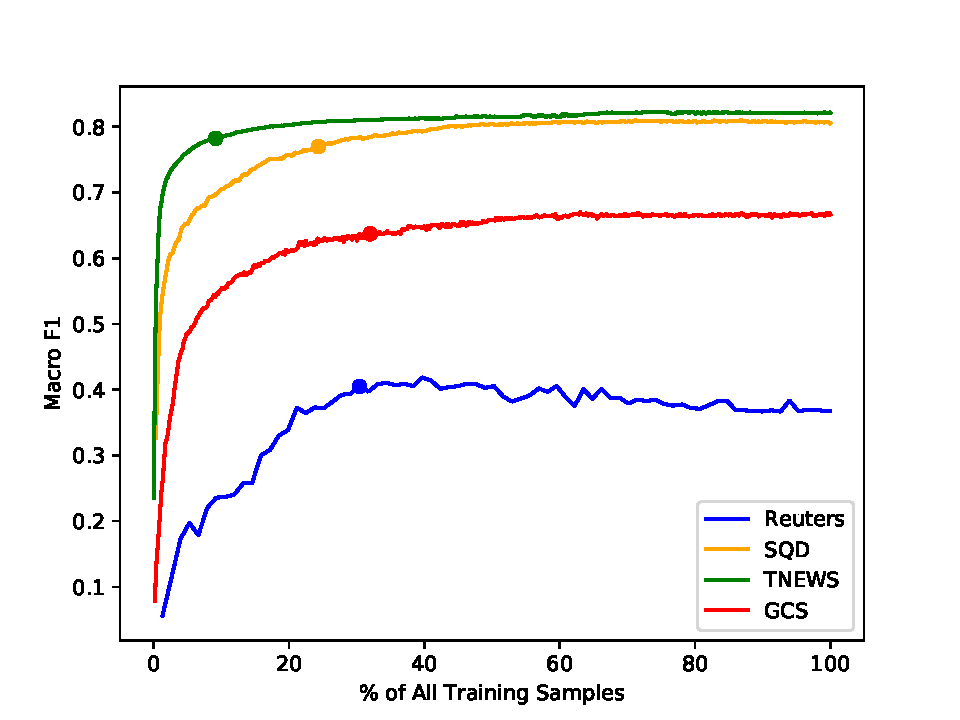
\includegraphics[scale=0.3]{figs/all_radiusfreq.pdf}
%	\caption{Training using Random Uncertainty with Freq}
%	\label{fig:all_radiusfreq}
%\end{figure}
\begin{table}[th]
	\scriptsize
	\centering
	\begin{tabular}{ccc}
		\toprule
		Dataset & \% of All Training Samples & Required Samples \\ \hline
		Reuters & 82.08   &  6,200 \\
		SQD     & 28.44   &  9,100 \\
		TNEWS   & 20.57    &  55,100 \\
		GCS     & 68.09   &  35,100 \\
		Biomedical & 43.13 & 6,900\\
		StackOverflow & 3.44 &550 \\
		SearchSnippets & 24.31 & 2,400 \\
		\bottomrule
	\end{tabular}
	\caption{\% samples and \# samples required to reach 95\% of the best accuracy (using fastText)}
	\label{table:all_radiusfreq}
\end{table}


Before evaluation, we first motivate why active learning is necessary for 
many-class classification problems. We first run the classification using full training data
on 8 datasets and record their upperbound F1 scores. Then, we apply our 
random sampling strategy from 100 samples up to all data.  
%As Fig ~\ref{fig:all_radiusfreq} shows, 
%All curves tend to saturate before 30\% of all data,
%with TNEWS using only 9.18\%.
\tabref{table:all_radiusfreq} shows the percentage of all data needed 
to label to reach 95\% of best accuracy. 
In all cases, we can stop labeling very early, sometimes as early as 3.44\% of
training data. 

We use traditional AL strategies as well as our proposed methods on $7$ datasets. 
In addition, we tuned some of the strong methods with class frequency and treat them as new methods. The performance of the 16 methods on 8 datasets is shown in a few tables. \tabref{table:auc_ft}, \tabref{table:auc_bert}, \tabref{table:auc_cnn} and \tabref{table:auc_lstm} presents the results on the above 7 datasets using fastText, BERT, CNN as well as LSTM with attention (denoted as LSTM+ATTN) respectively. To illustrate our results, we plot the macro-F1 curves of 
all competing methods on 7 datasets (\figref{fig:acc_all}, \figref{fig:acc_all_bert}, \figref{fig:acc_all_lstm}, \figref{fig:acc_all_cnn}).

\begin{table*}[th]
	\centering
	\scriptsize
	\begin{tabular}{ccccccccc}
		\toprule
		Method & Reuters & HuffPost & Biomedical & SearchSnippets & Emoji & TNEWS & GCS & Book\\ \hline
		Random Sampling & 365.96 & 280.51 & 1601.06 & 2397.09 & 355.35 & 1673.69 & 892.04 & 965.12\\ \hline
		
		Least Confidence & \textbf{1003.46} & 288.42 & 1448.65 & \textbf{2577.79} & 321.99 & 1597.56 & 900.37 & 1118.76\\
		LC with Freq & 676.71 & 301.71 & 1503.77 & 2485.63 & 320.62 & 1695.25 & 748.59 & 818.2\\
		LC with Sqrtfreq & 890.78 & 291.19 & 1456.77 & 2556.63 & 331.6 & 1702.49 & 858.19 & 917.43\\  \hline
		
		K-center Greedy & 761.08 & 277.13 & 1428.09 & 2542.13 & \textbf{357.15} & 1555.7 & 901.12 & 1004.73\\
		KG with Freq & 871.98 & 284.63 & \textbf{1626.72} & 2566.22 & 345.34 & 1730.05 & 1042.11 & 1122.64\\
		KG with Sqrtfreq & 831.09 & 282.89 & 1612.83 & 2568.58 & 346.49 & \textbf{1731.64} & 1039.3 & 1097.55\\ \hline
		Uncertainty Sampling & 957.36 & 284.99 & 1466.59 & 2569.79 & 315.03 & 1694.25 & 980.86 & 1103.01\\
		US with Freq & 938.21 & 287.41 & 1584.7 & 2551.31 & 334.92 & 1720.2 & 1070.12 & 1119.7\\
		US with Sqrtfreq & 959.33 & 284.8 & 1583.2 & 2569.79 & 338.5 & 1724.03 & 1053.67 & 1163.23\\ \hline
		Weighted Uncertainty & 844.36 & \textbf{310.28} & 1489.05 & 2518.29 & 309.94 & 1672.12 & 1045.88 & 1135.19\\
		WU with Freq & 848.42 & 293.8 & 1530.14 & 2504.46 & 339.46 & 1710.65 & \textbf{1087.23} & 1126.69\\
		WU with Sqrtfreq & 892.98 & 288.48 & 1526.9 & 2518.56 & 338.29 & 1701.27 & 1064.86 & 1123.7\\ \hline
		Radius Uncertainty & 989.6 & 286.74 & 1517.86 & 2569.5 & 320.1 & 1699.65 & 986.55 & 1110.52\\
		RU with Freq & 946.78 & 297.8 & 1570.96 & 2555.48 & 330.84 & 1717.35 & 1073.74 & 1143.98\\
		RU with Sqrtfreq & 962.77 & 285.12 & 1573.23 & 2561.74 & 327.67 & 1720.39 & 1055.76 & \textbf{1165.94}\\
		\hline
	\end{tabular}
\caption{AUC* of AL methods on seven datasets running from 100 to 3000 with batch size 100 using fastText}
\label{table:auc_ft}
\end{table*}


\begin{table*}[th]
	\centering
	\scriptsize
	\begin{tabular}{cccccccc}
		\toprule
		Method & Reuters & SQD & Bio & Search & Stack & TNEWS & GCS \\ \hline
		Random Sampling & 129.15 & 930.86 & 784.26 & 2338.62 & \textbf{1496.22} & 1857.81 & 111.26\\
		Least Confidence & \textbf{329.15} & 735.91 & 798.96 & \textbf{2398.02} & 1360.95 & \textbf{1936.98} & \textbf{254.53}   \\
		K-center Greedy & 194.42 & 568.48 & 466.34 & 2215.89 & 1030.4 & 1760.38 & 87.11  \\ \hline
		Weighted Uncertainty & 235.56 & 930.31 & 622.36 & 2226.46  & 1419.58 & 1796.18 & 119.83 \\
		WU with Freq & 229.85 & 909.02 & 619.66 & 2300.18  & 1420.0 & 1806.31 & 150.05 \\
		WU with Sqrtfreq & 244.78 & \textbf{944.72} & 630.44 & 2272.93 & 1366.09  & 1805.28 & 153.33 \\ \hline
		Uncertainty Sampling & 305.45 & 729.55 & 791.03 & 2361.41 & 1297.7  & 1871.4 & 248.78  \\
		US with Freq & 293.36 & 910.33 & 803.1 & 2359.81 & 1418.15 & 1920.04 & 218.89   \\
		US with Sqrtfreq & 300.36 & 935.45 & 831.62  & 2371.52 & 1426.9 & 1926.14 & 207.63 \\ \hline
		Radius Uncertainty & 321.55 & 786.11 & 784.11 & 2372.95& 1354.27 & 1927.58 & 225.19  \\
		RU with Freq & 316.68 & 899.05 & 806.54 & 2376.49 & 1437.71& 1891.11 & 184.55   \\
		RU with Sqrtfreq & 326.17 & 879.29 & \textbf{826.32} & 2359.01 & 1429.29 & 1882.04 &  204.51\\
		\hline
	\end{tabular}
\caption{AUC* of AL methods on seven datasets up to 3000 samples using BERT}
\label{table:auc_bert}
\end{table*}

\begin{table*}[th]
	\centering
	\scriptsize
	\begin{tabular}{cccccccc}
		\toprule
		Method & Reuters & SQD & Bio & Search & Stack & TNEWS & GCS \\ \hline
		Random Sampling & 371.58  & 393.02 & 1178.19 & 2351.72 & 1940.22 & 1264.98 & 151.31  \\
		Least Confidence & 367.81 & 380.96  & 1181.68 & 2351.76 & 1941.66 & 1269.46 & 146.92 \\
		K-center Greedy & 385.42 & 394.37  & 1169.59  & 2355.37 & 1931.09 & 1242.46 & 146.21 \\ \hline
		Weighted Uncertainty & \textbf{388.76} & 383.29 & 1168.16 & 2351.09 & 1922.21 & 1257.84 & \textbf{157.06 }  \\
		WU with Freq & 378.51 & 365.25  & 1166.58 & 2364.41 & 1936.04 & 1254.82 & 152.93  \\
		WU with Sqrtfreq & 371.77 & 377.0 & 1182.11 & \textbf{2382.61} & 1926.61 & 1277.22 & 148.55  \\ \hline
		Uncertainty Sampling & 373.65 & \textbf{399.53} & 1159.86 & 2358.26  & 1930.83 & 1263.03 & 154.94 \\
		US with Freq & 385.44 & 384.71 & 1179.12  & 2349.46 & 1927.75 & \textbf{1278.37} & 150.69  \\
		US with Sqrtfreq & 315.3 & 389.08 & 1176.63 & 2375.11 & \textbf{1953.33} & 1263.01 & 152.03 \\ \hline
		Radius Uncertainty & 382.75 & 382.45 & 1173.75 & 2367.49 & 1937.85 & 1254.72 & 156.88   \\
		RU with Freq & 387.87 & 347.69 & 1173.81 & 2374.25 & 1926.42 & 1264.93 &  152.7 \\
		RU with Sqrtfreq & 387.47 & 372.75 & \textbf{1183.23} & 2372.52 &  1925.59 & 1253.49 & 156.27 \\
		\hline
	\end{tabular}
\caption{AUC* of AL methods on seven datasets up to 3000 samples using CNN}
\label{table:auc_cnn}
\end{table*}

\begin{table*}[th]
	\centering
	\scriptsize
	\begin{tabular}{cccccccc}
		\toprule
		Method & Reuters & SQD & Bio & Search & Stack & TNEWS & GCS \\ \hline
		Random Sampling & 430.98 & 1490.12 & 1409.95 & 2521.58 & 2328.09 & 956.06 & 138.01\\
		Least Confidence & 430.72 & 1491.45 & 1428.33 & 2507.47 & 2344.13 & 946.2 & 139.45\\
		K-center Greedy & \textbf{446.15} & \textbf{1527.33} & 1425.22 & 2508.08 & \textbf{2348.03} & 931.23 & 136.74\\ \hline
		Weighted Uncertainty & 424.03 &  1503.76 & 1427.31 & 2505.19 & 2333.19 & 951.12 & 134.12\\
		WU with Freq & 418.37 & 1486.4 & 1423.83 & 2494.09 & 2333.11 & 947.66 & 132.02\\
		WU with Sqrtfreq & 445.81 & 1489.16 & 1431.63 & 2519.35 & 2343.46 & \textbf{962.61} & 137.3\\ \hline
		Uncertainty Sampling & 438.05 & 1498.27 & 1426.41 & 2509.67 & 2341.75 & 940.49 & 131.9\\
		US with Freq & 435.48 & 1489.11 & 1425.03 & \textbf{2534.85} & 2331.67 & 944.99 & 133.8\\
		US with Sqrtfreq & 437.06 & 1510.34 & 1407.88 & 2525.17 & 2335.28 & 972.2 & \textbf{141.68}\\ \hline
		Radius Uncertainty & 439.02 & 1503.02 & \textbf{1430.13} & 2519.31 & 2347.34 & 951.92 & 123.86\\
		RU with Freq & 432.9 & 1499.66 & 1427.86 & 2509.21 & 2347.4 & 944.0 & 134.01\\
		RU with Sqrtfreq & 442.56 & 1482.94 & 1416.99 & 2493.21 & 2343.74 & 931.82 & 136.6\\
		\hline
	\end{tabular}
\caption{AUC* of AL methods on seven datasets running from 100 to 3000 with batch size 100 using LSTM}
\label{table:auc_lstm}
\end{table*}

\begin{table}[th]
	\centering
	\scriptsize
	\begin{tabular}{ccccc}
		\toprule
		Method & BERT & fastText & CNN & LSTM \\  \hline
		Random Sampling & 0.27 & 0.28 & 0.2 & 0.2\\
		Least Confidence & \textbf{0.63} & 0.35 & 0.22 & 0.22\\
		K-center Greedy & 0.08 & 0.10 & 0.18 & \textbf{0.5}\\ \hline
		Weighted Uncertainty & 0.13 & 0.23 & \textbf{0.37} & 0.17\\
		WU with freq & 0.13 & 0.29 & 0.14 & 0.11\\
		WU with sqrtfreq & 0.24 & 0.2 & 0.35 & 0.4\\ \hline
		Uncertainty Sampling & 0.2 & 0.18 & 0.27 & 0.15\\
		US with Freq & 0.2 & 0.27 & 0.29 & 0.24\\
		US with Sqrtfreq & 0.39 & \textbf{0.36} & 0.33 & 0.48\\ \hline
		Radius Uncertainty & 0.26 & 0.21 & 0.21 & 0.27\\
		RU with Freq & 0.29 & 0.35 & 0.22 & 0.21\\
		RU with Sqrtfreq & 0.28 & 0.26 & 0.31 & 0.15\\
		\hline
	\end{tabular}
	\caption{MRR score of AL methods on seven datasets using different classifiers.}
	\label{table:mrr}
\end{table}


To compare the performance difference on the number of classes in the task, 
we calculate the MRR score by aggregating datasets with the same class number. 
We do this for curves that ends at 3000 sample points to save time. 
The results are included in \tabref{table:mrr}. We have two observations.

%\KZ{Insert a table with three columns (no freq, +freq, +sqrtfreg), rows are
%US, WU, Radius, each cell is the MRR of the method aggregated on all
%the datasets for 3000}


The \textbf{first} observation is that adding frequency adjustment does help on all 
methods including uncertainty sampling, weighted uncertainty as well as radius uncertainty in most cases.  
% Since frequency adjustment is specially designed for many-class scenarios, 
% we only compare the MRR scores on the original datasets. 
% As \figref{fig:mrr} shows, all the orange and green bars are higher than the blue bars. 
% In other words, methods have increased their score to some extent after applying frequency 
% adjustment regardless of the ending point.

% \begin{figure*}
% 	\centering
% 	%\subfloat[Complaint]{\includegraphics[width=0.2\textwidth]{figs/complaint.eps}}
% 	\subfloat[AL up to 1000 samples]{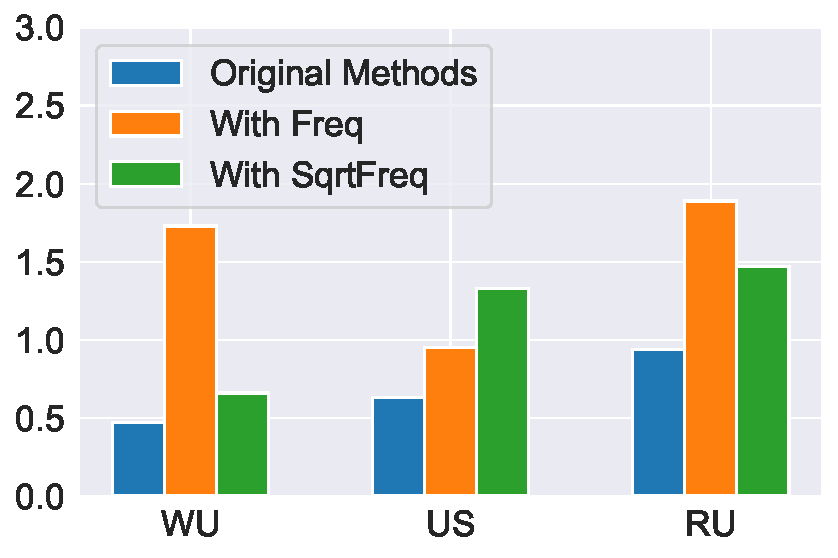
\includegraphics[width=0.3\textwidth]{figs/mrr_1000.pdf}}
% 	\subfloat[AL up to 2000 samples]{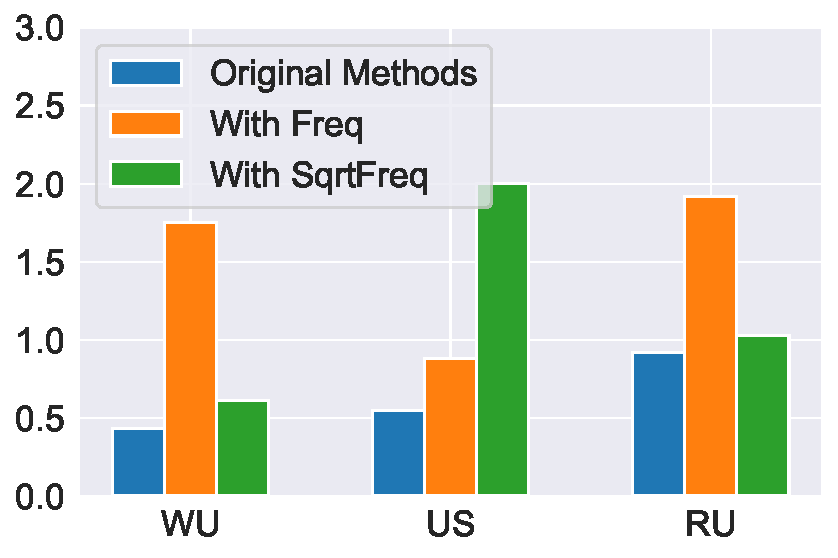
\includegraphics[width=0.3\textwidth]{figs/mrr_2000.pdf}}
% 	\subfloat[AL up to 3000 samples]{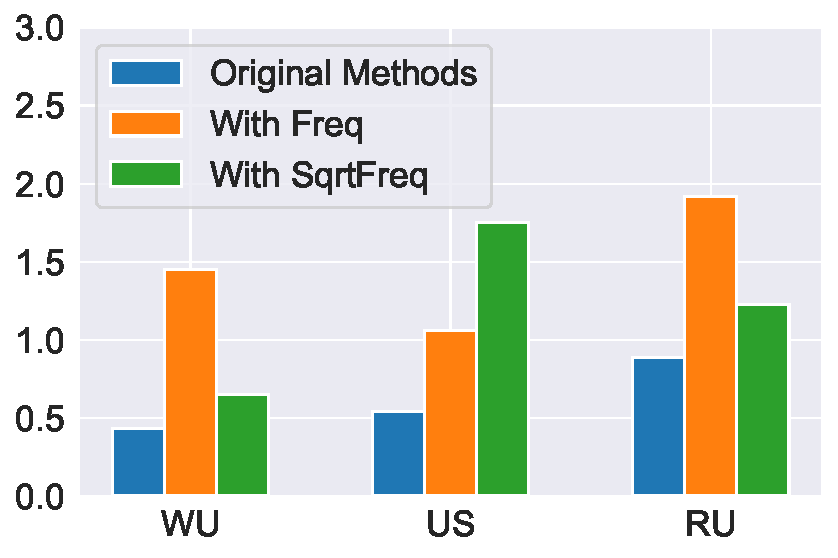
\includegraphics[width=0.3\textwidth]{figs/mrr_3000.pdf}}
% 	\caption{MRR scores before and after applying frequency adjustment on WU, US and RU. EP = 1000,2000,3000 denotes for AL up to 1000,2000,3000 respectively.} 
% 	\label{fig:mrr}
% \end{figure*}

% The \textbf{second} finding is that our proposed variant \textbf{uncertainty sampling with frequency adjustment} and \textbf{radius uncertainty with frequency adjustment} perform well in all datasets and at different active learning processes. 
% They outperform all the traditional methods. From \tabref{table:mrr}, we can conclude \textbf{US with Freq} works pretty well on small classes especially the class number is small. When it comes to many-class classification, our proposed \textbf{RU with Freq} has achieved good results, achieving highest performance if we actively learn up to  1000 and 3000 samples, and
% second highest if we learn up to 2000.
% Besides, we can see the tendency that the MRR score of traditional AL which obtains 
% good results on small datasets drop continually with the increase of class number. 
% For instance, for uncertainty sampling, MRR score changes from 1.68 to 0.63, 
% 0.99 to 0.55 and 1.44 to 0.54 separately when AL stops at 1000, 2000 and 3000.

The \textbf{second} finding is that the harder the dataset is, the more useful AL is. \figref{fig:avgsample_ratio} shows that when \#samples/class increase, the difference of AUC* between best AL method and Random decreases. \tabref{table:pearson} indicates that for all the models that we tested, lower upperbound (i.e. the harder the dataset is) widen the gap between best method and Random. The low p-value shows such conclusion is statistically significant.

% Finally, we discover that the new methods work particularly well when 
% the number of classes is large, while the advantages of traditional ones diminish. 
% \figref{fig:trend} depicts that with the increase of classes, traditional strategies 
% like WU,US and KG drops significantly but our proposed variants gains considerable margin. 
% However, there does exist some noises, for method RU with sqrtFreq, 
% the performance doesn't increase in accordance to MRR. 
% After looking into the AUC* of this method, 
% we can conclude that the MRR score drops significantly due to its poor performance in SQD. SQD is a relatively long and 
% difficult datasets which most methods fail to perform well on. Moreover,
% the distribution of SQD is even, leading to the smoothing strategy meaningless.
% So, this is a reasonable phenomenon and the general principle we discovered so far
% still applies.

% \begin{figure}[th]
% 	\centering
% 	\subfloat[][
% 	Drop of MRR score of tradition AL methods]{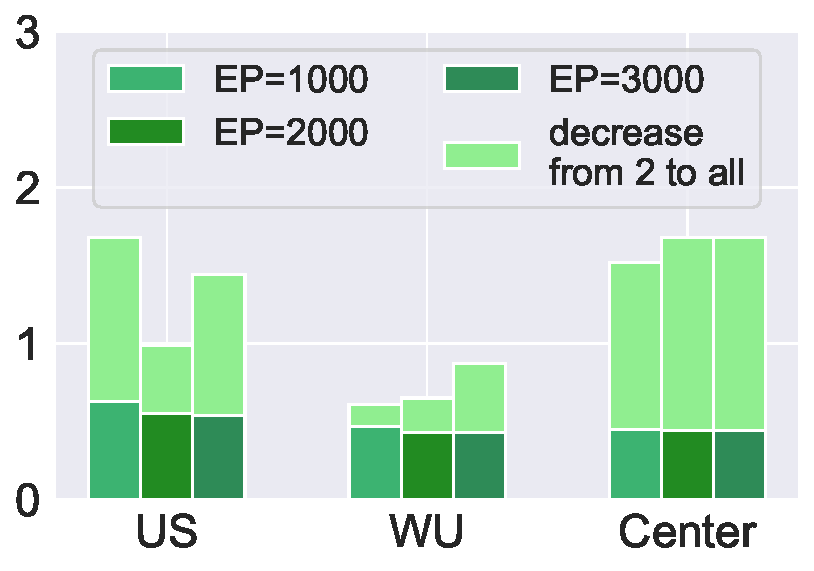
\includegraphics[width=0.25\textwidth]{figs/drop.pdf}}
% 	\subfloat[][ 
% 	Increase of MRR score of Radius-based methods
% 	($\triangledown$ indicates decreasing)]{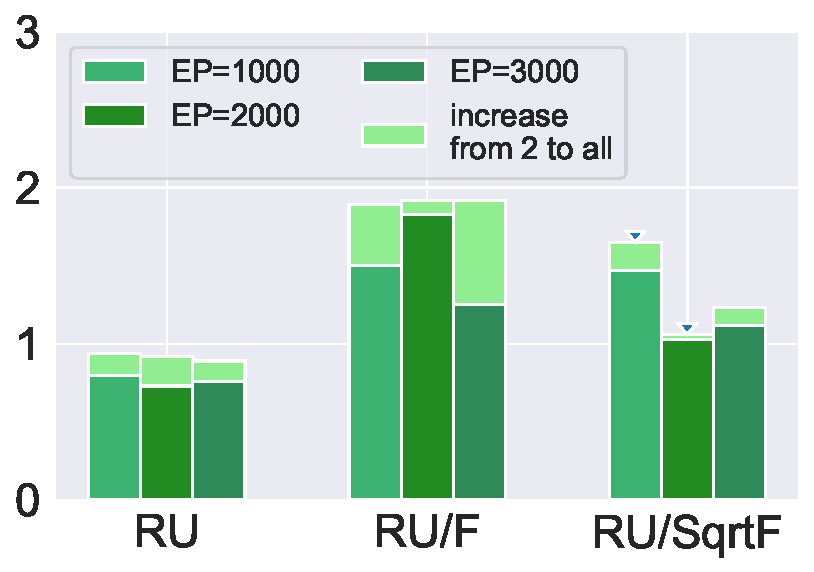
\includegraphics[width=0.25\textwidth]{figs/plus.pdf}}
% 	\caption{Difference in MRR scores between 2-class and all-class problems  (F is Freq and SqrtF is Sqrtfreq)}
% 	\label{fig:trend}
% \end{figure}

% \subsection{Effects of Frequency Adjustment}
% Figure ~\ref{fig:legend} shows the legend of all result figures. 
% Figure ~\ref{fig:complaint_exp1},~\ref{fig:reuters_exp1},~\ref{fig:so_exp1},~\ref{fig:tnews_exp1},~\ref{fig:yanjing_exp1} display Experiment (a) results and Figure ~\

% \begin{figure}[h]
% 	\centering
% 	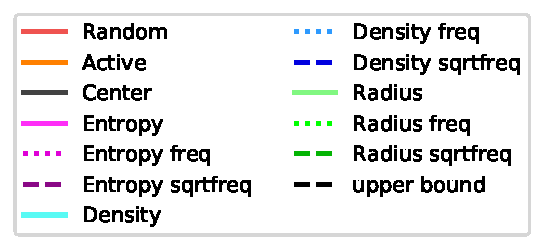
\includegraphics[scale=0.5]{figs/legend.pdf}
% 	\caption{Legend of Result Figures. In following figures, 
% unless otherwise noted, \textit{x} denotes the size of training samples 
% and \textit{y} denotes macro-average F1 score of the classifier trained
% on the corresponding trainig sample.}
% 	\label{fig:legend}
% \end{figure}

% \begin{figure}[h]
% 	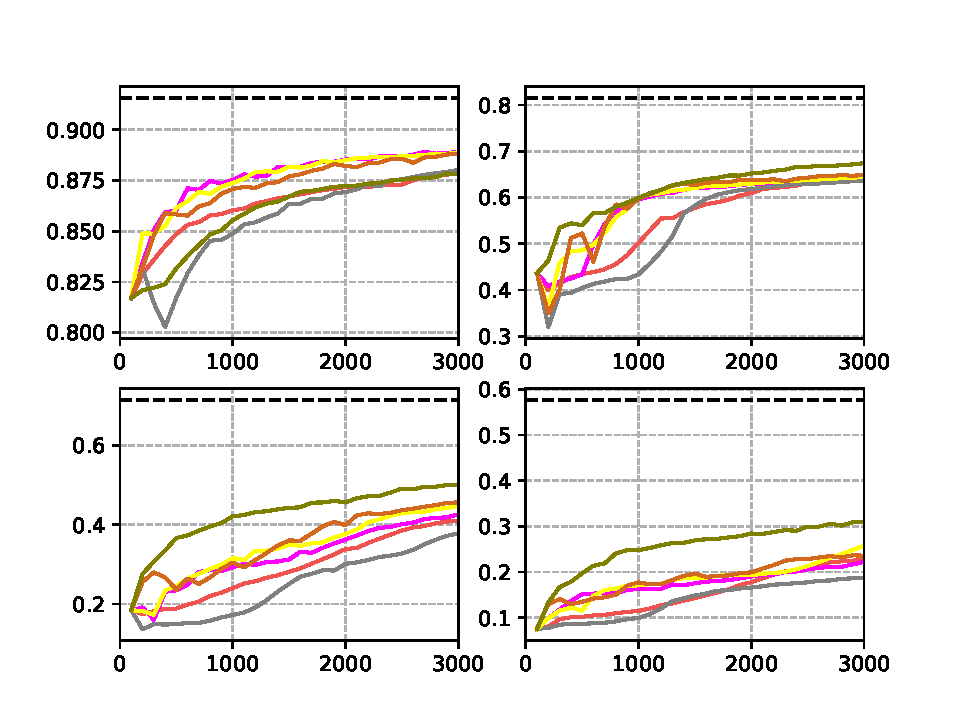
\includegraphics[scale=0.5]{figs/complaint_exp1.pdf}
% 	\caption{Exp (a) Result of Complaint. From left to right, from upper to lower is 2, 5, 10 and all classes.}
% 	\label{fig:complaint_exp1}
% \end{figure}

% \begin{figure}[h]
% 	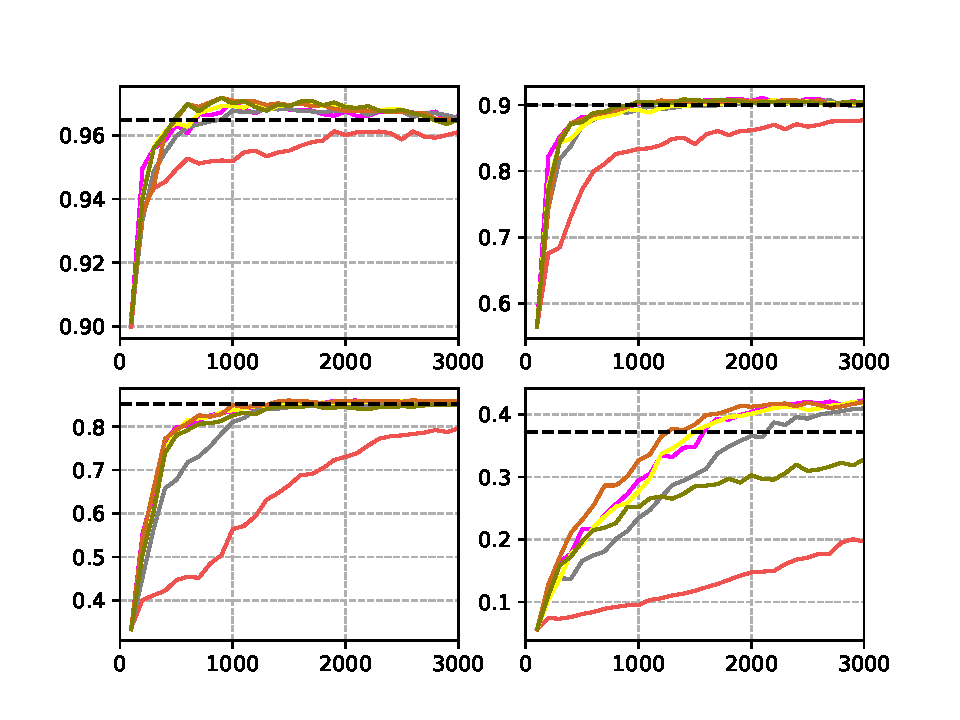
\includegraphics[scale=0.5]{figs/reuters_exp1.pdf}
% 	\caption{Exp (a) Result of Reuters}
% 	\label{fig:reuters_exp1}
% \end{figure}

% \begin{figure}[h]
% 	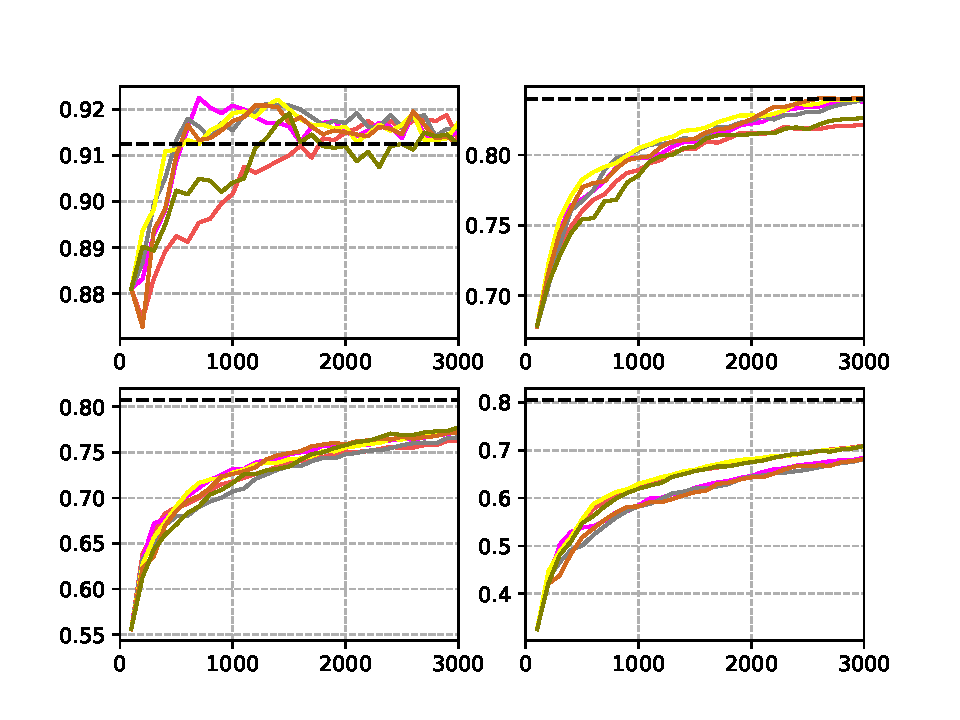
\includegraphics[scale=0.5]{figs/so_exp1.pdf}
% 	\caption{Exp (a) Result of SO}
% 	\label{fig:so_exp1}
% \end{figure}

% \begin{figure}[h]
% 	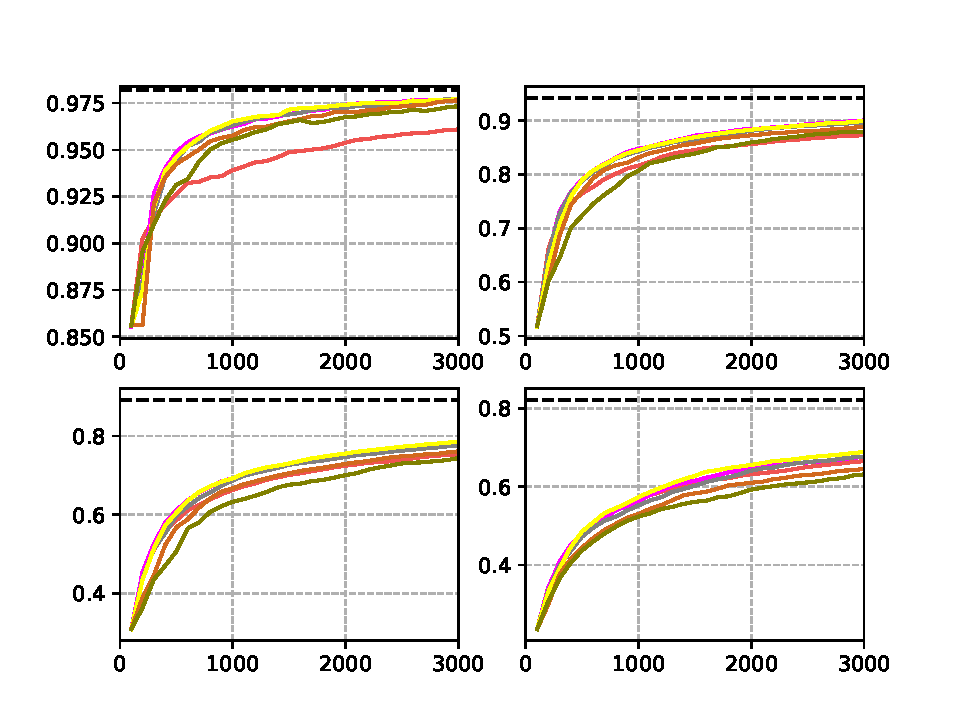
\includegraphics[scale=0.5]{figs/tnews_exp1.pdf}
% 	\caption{Exp (a) Result of TNEWS}
% 	\label{fig:tnews_exp1}
% \end{figure}

% \begin{figure}[h]
% 	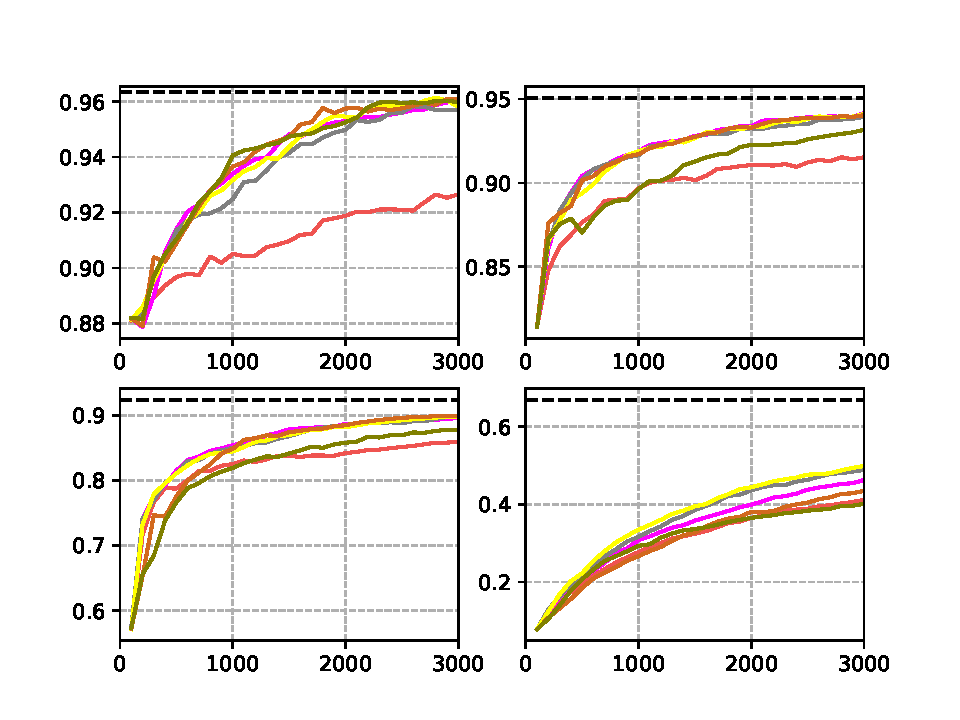
\includegraphics[scale=0.5]{figs/yanjing_exp1.pdf}
% 	\caption{Exp (a) Result of GCS}
% 	\label{fig:yanjing_exp1}
% \end{figure}


% \subsection{Radius vs. Other state-of-the-art methods}
% \KZ{Here we show the results of applying freq to various
% base AL methods.}

% \begin{figure}[h]
% 	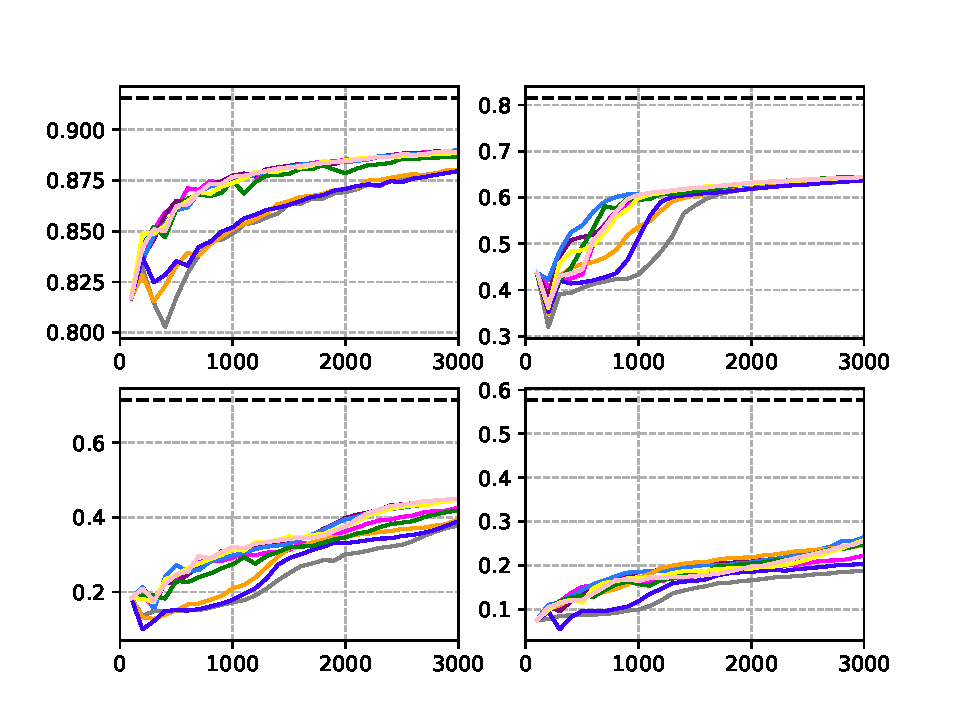
\includegraphics[scale=0.5]{figs/complaint_exp2.pdf}
% 	\caption{Exp (b) Result of Complaint}
% 	\label{fig:complaint_exp2}
% \end{figure}

% \begin{figure}[h]
% 	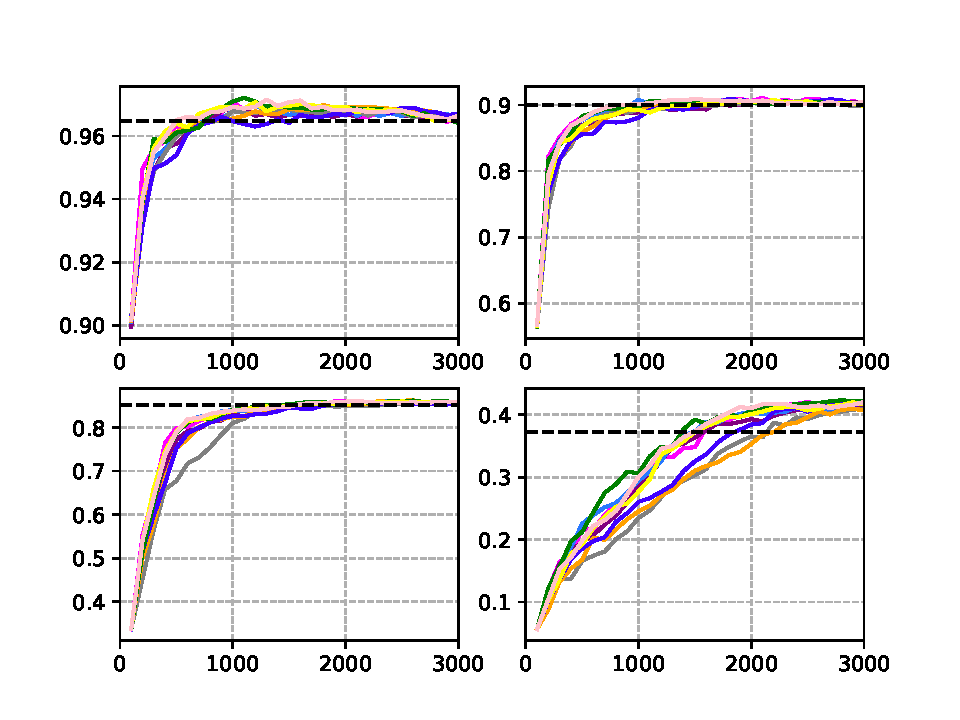
\includegraphics[scale=0.5]{figs/reuters_exp2.pdf}
% 	\caption{Exp (b) Result of Reuters}
% 	\label{fig:reuters_exp2}
% \end{figure}

% \begin{figure}[h]
% 	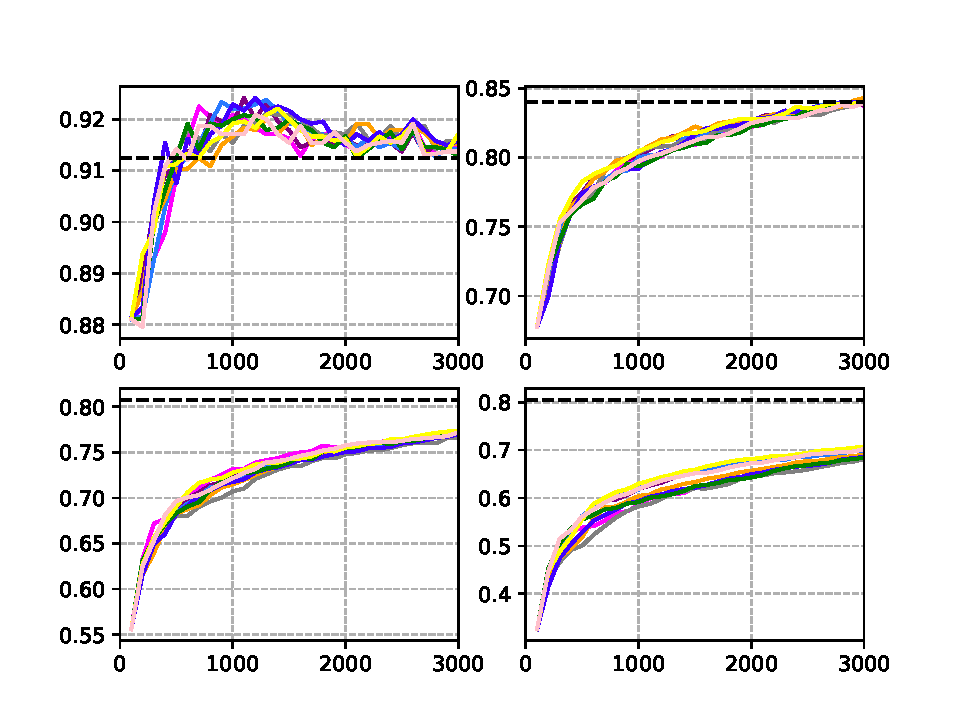
\includegraphics[scale=0.5]{figs/so_exp2.pdf}
% 	\caption{Exp (b) Result of SO}
% 	\label{fig:so_exp2}
% \end{figure}

% \begin{figure}[h]
% 	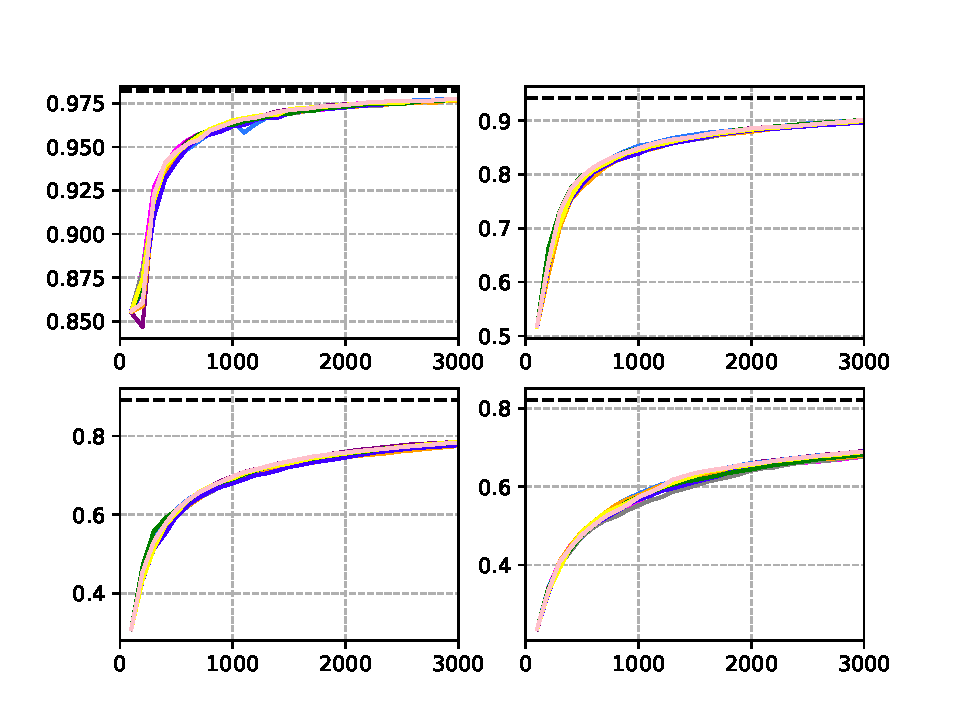
\includegraphics[scale=0.5]{figs/tnews_exp2.pdf}
% 	\caption{Exp (b) Result of TNEWS}
% 	\label{fig:tnews_exp2}
% \end{figure}

% \begin{figure}[h]
% 	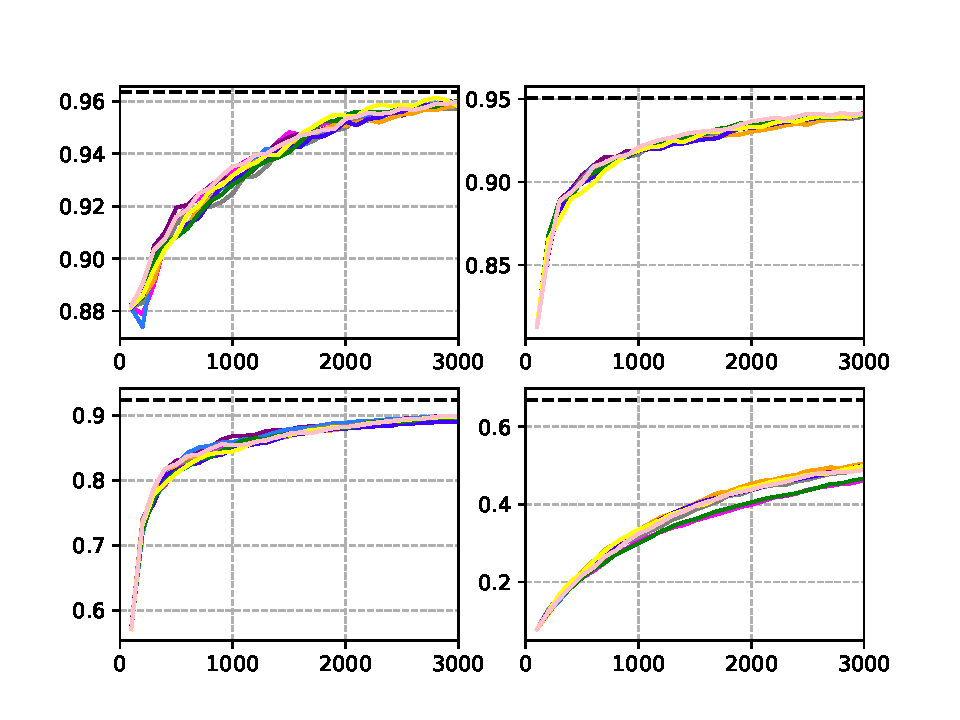
\includegraphics[scale=0.5]{figs/yanjing_exp2.pdf}
% 	\caption{Exp (b) Result of GCS}
% 	\label{fig:yanjing_exp2}
% \end{figure}

% \begin{table}[]
% 	\begin{tabular}{cc|cc}
% 		\hline
% 		Method           & Score  & Method           & Score\\ \hline
% 		Random           & 2.40 & Density           & 2.73 \\
% 		Active           & 3.11 &  Density freq     & 4.12  \\
% 		Center           & 5.52 &  Density sqrtfreq & 3.43  \\
% 		Entropy          & 6.89 &  Radius           & 5.57  \\
% 		Entropy freq     & 7.83 &  Radius freq      & 6.83  \\
% 		Entropy sqrtfreq & 6.21 &  Radius sqrtfreq  & 7.44  \\ \hline
% 	\end{tabular}
% \caption{Score of Methods summed over datasets and number of classes}
% \label{table:score}
% \end{table}

% \subsection{Effect from different number of classes}

% \begin{figure*}[th]
% 	\centering
% 	\subfloat[Complaint]{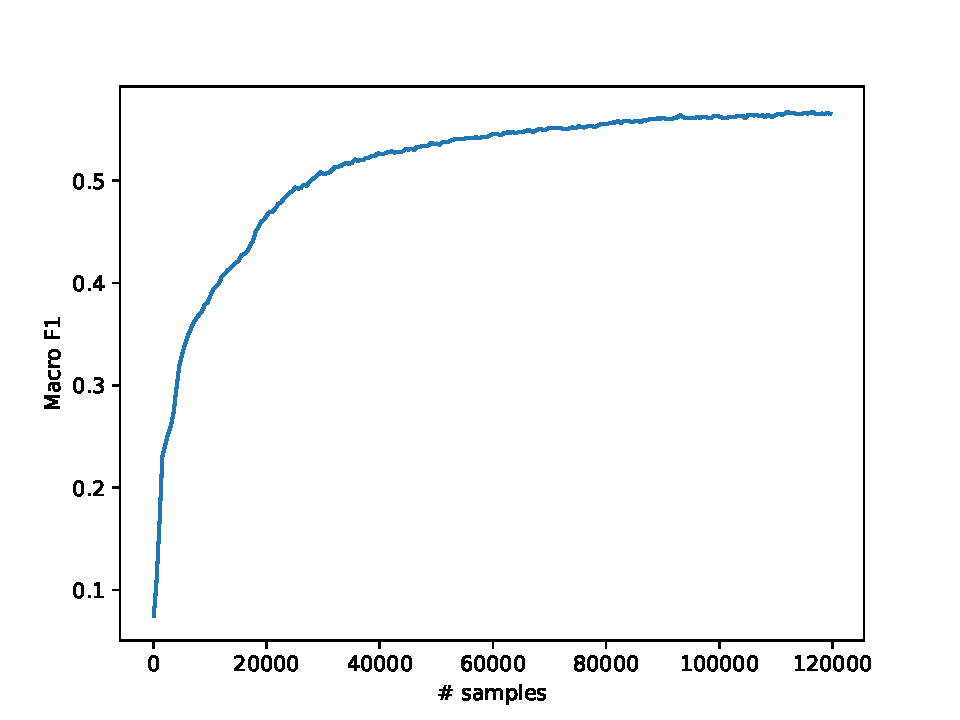
\includegraphics[width=0.2\textwidth]{figs/complaint_exp3.pdf}}
% 	\subfloat[Reuters]{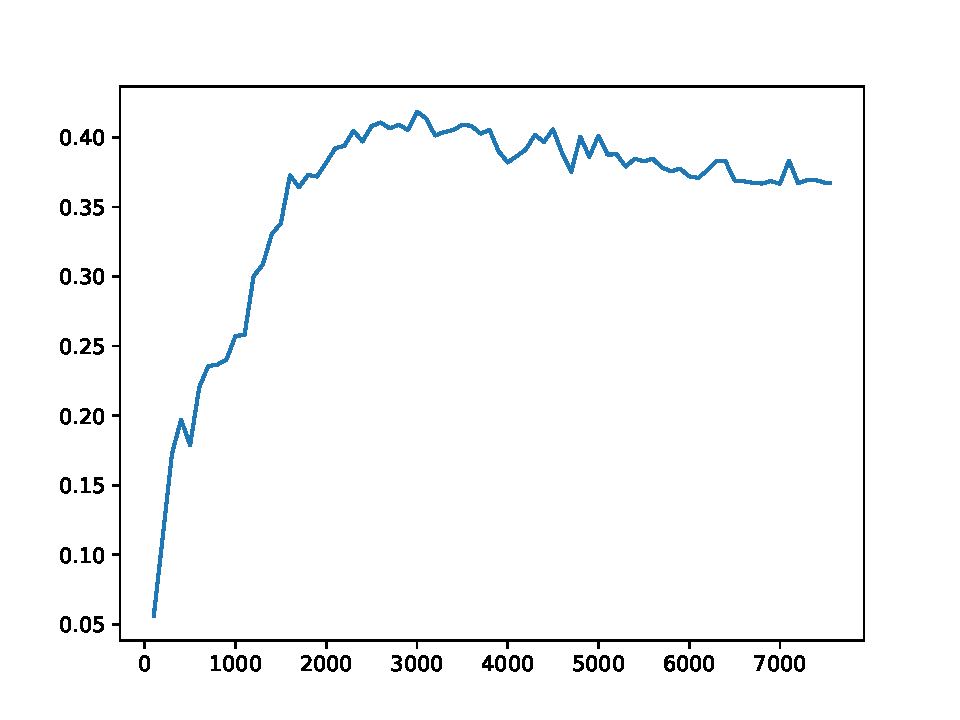
\includegraphics[width=0.2\textwidth]{figs/reuters_exp3.pdf}}
% 	\subfloat[SO]{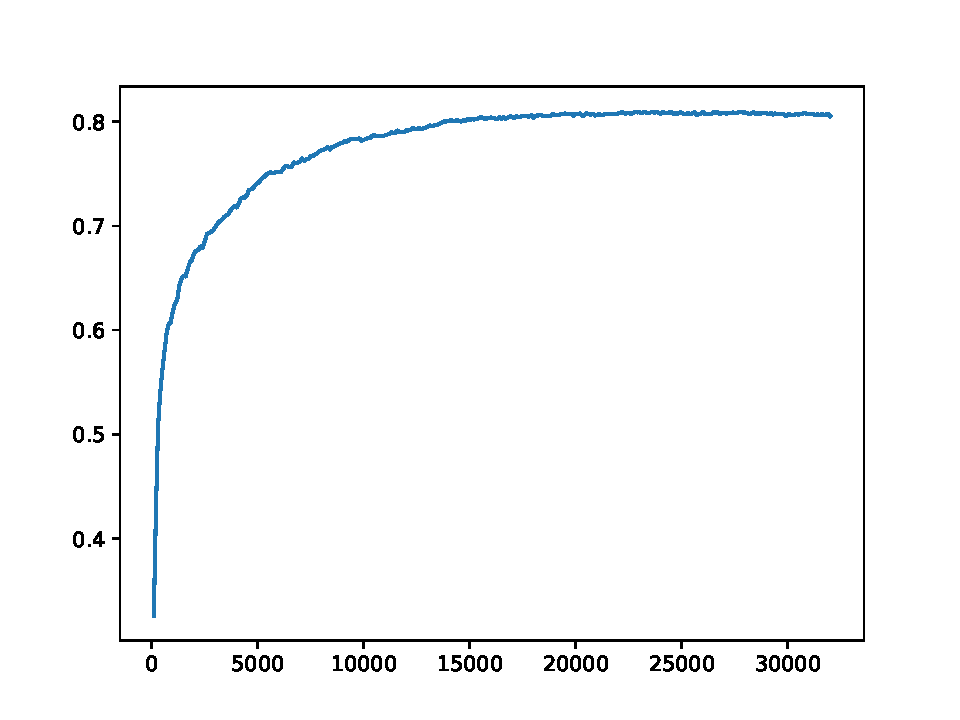
\includegraphics[width=0.2\textwidth]{figs/so_exp3.pdf}}
% 	\subfloat[TNEWS]{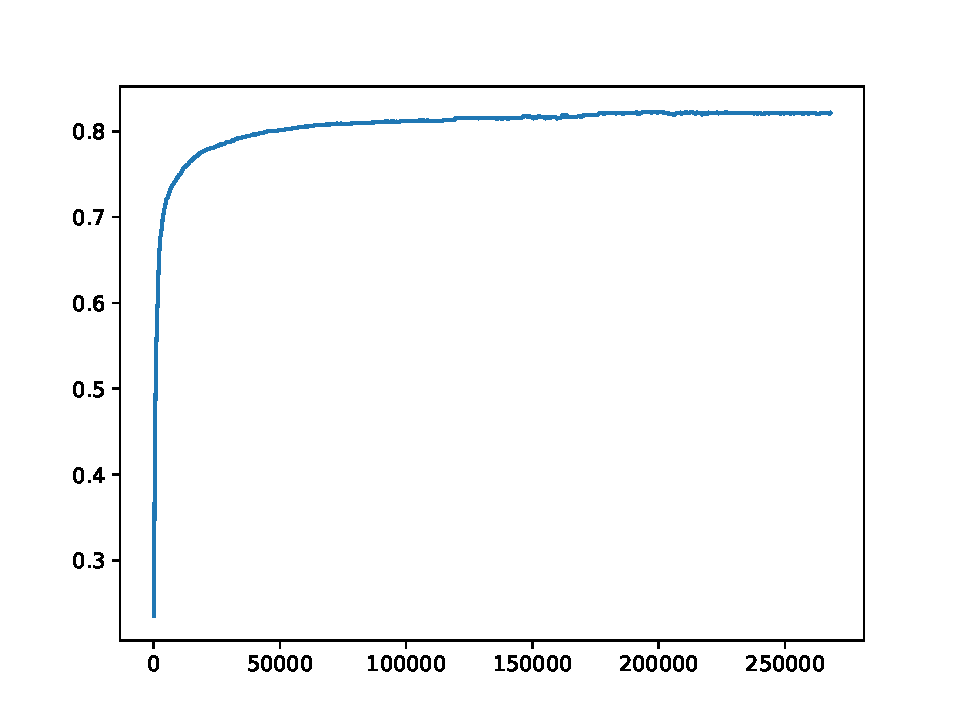
\includegraphics[width=0.2\textwidth]{figs/tnews_exp3.pdf}}
% 	\subfloat[GCS]{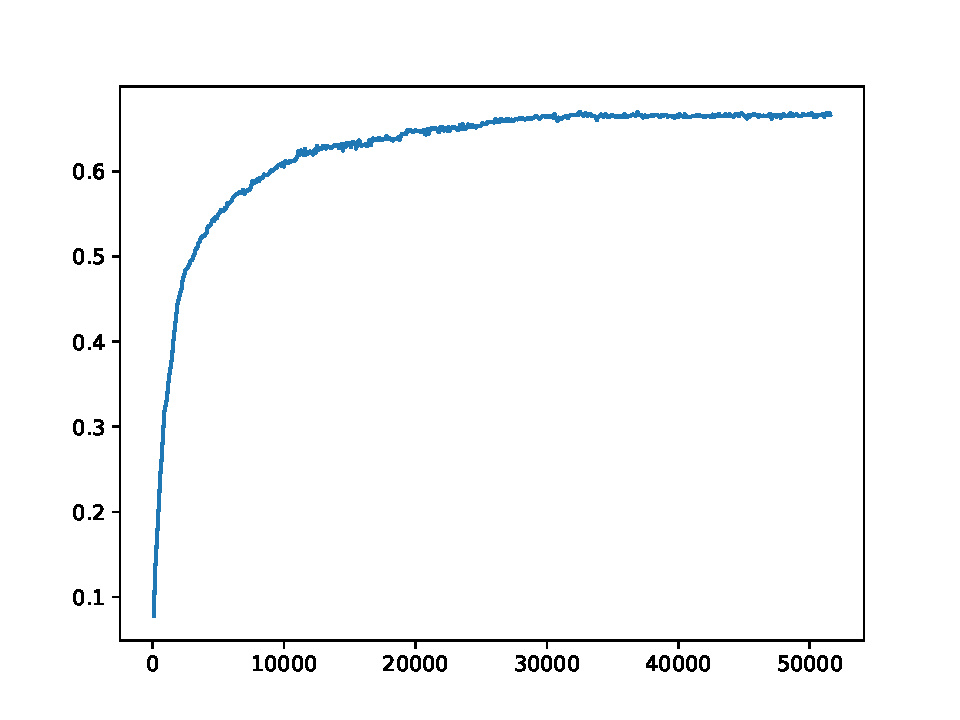
\includegraphics[width=0.2\textwidth]{figs/yanjing_exp3.pdf}}
% 	\caption{Exp (c) Result} 
% 	\label{fig:exp3}
% \end{figure*}
\begin{figure}[th!]%[!hbt]
\begin{center}
\subfloat[Legend]{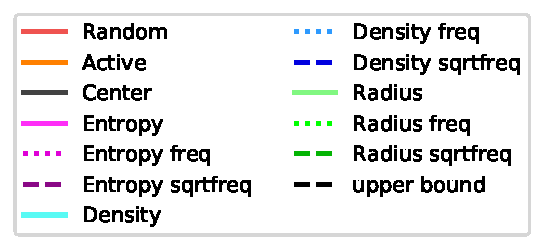
\includegraphics[scale=0.55]{figs/legend.pdf}}
\end{center}
\noindent
	\begin{center}
		\subfloat[Reuters]{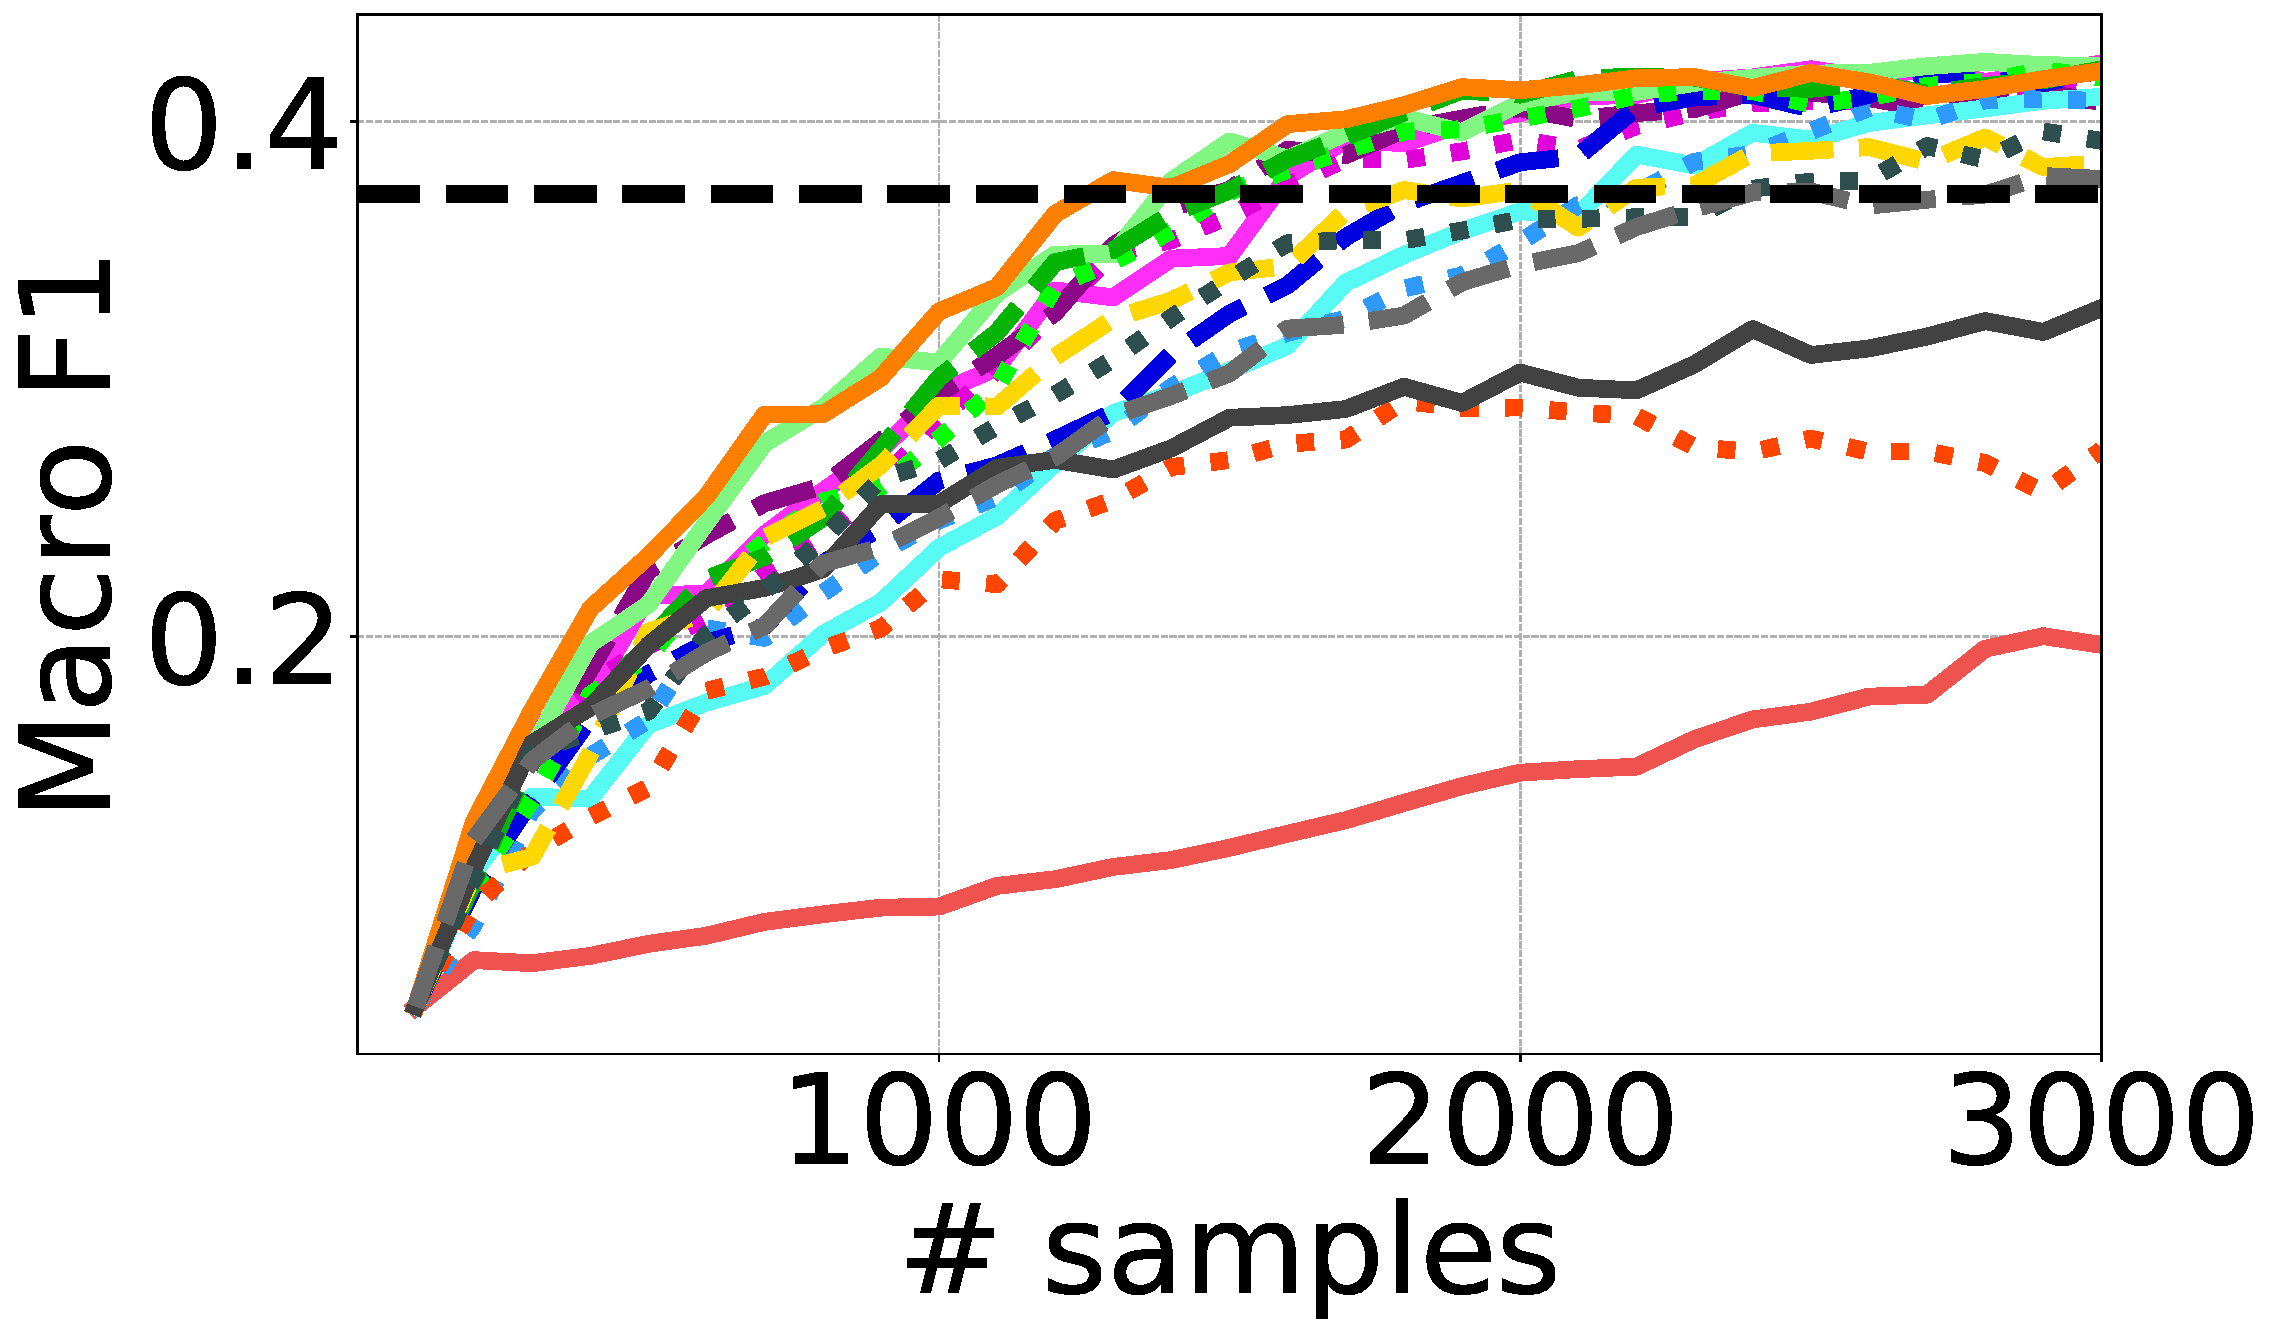
\includegraphics[width=0.24\textwidth]{figs/ft_reuters_new_acc_all.pdf}}
		\subfloat[HuffPost]{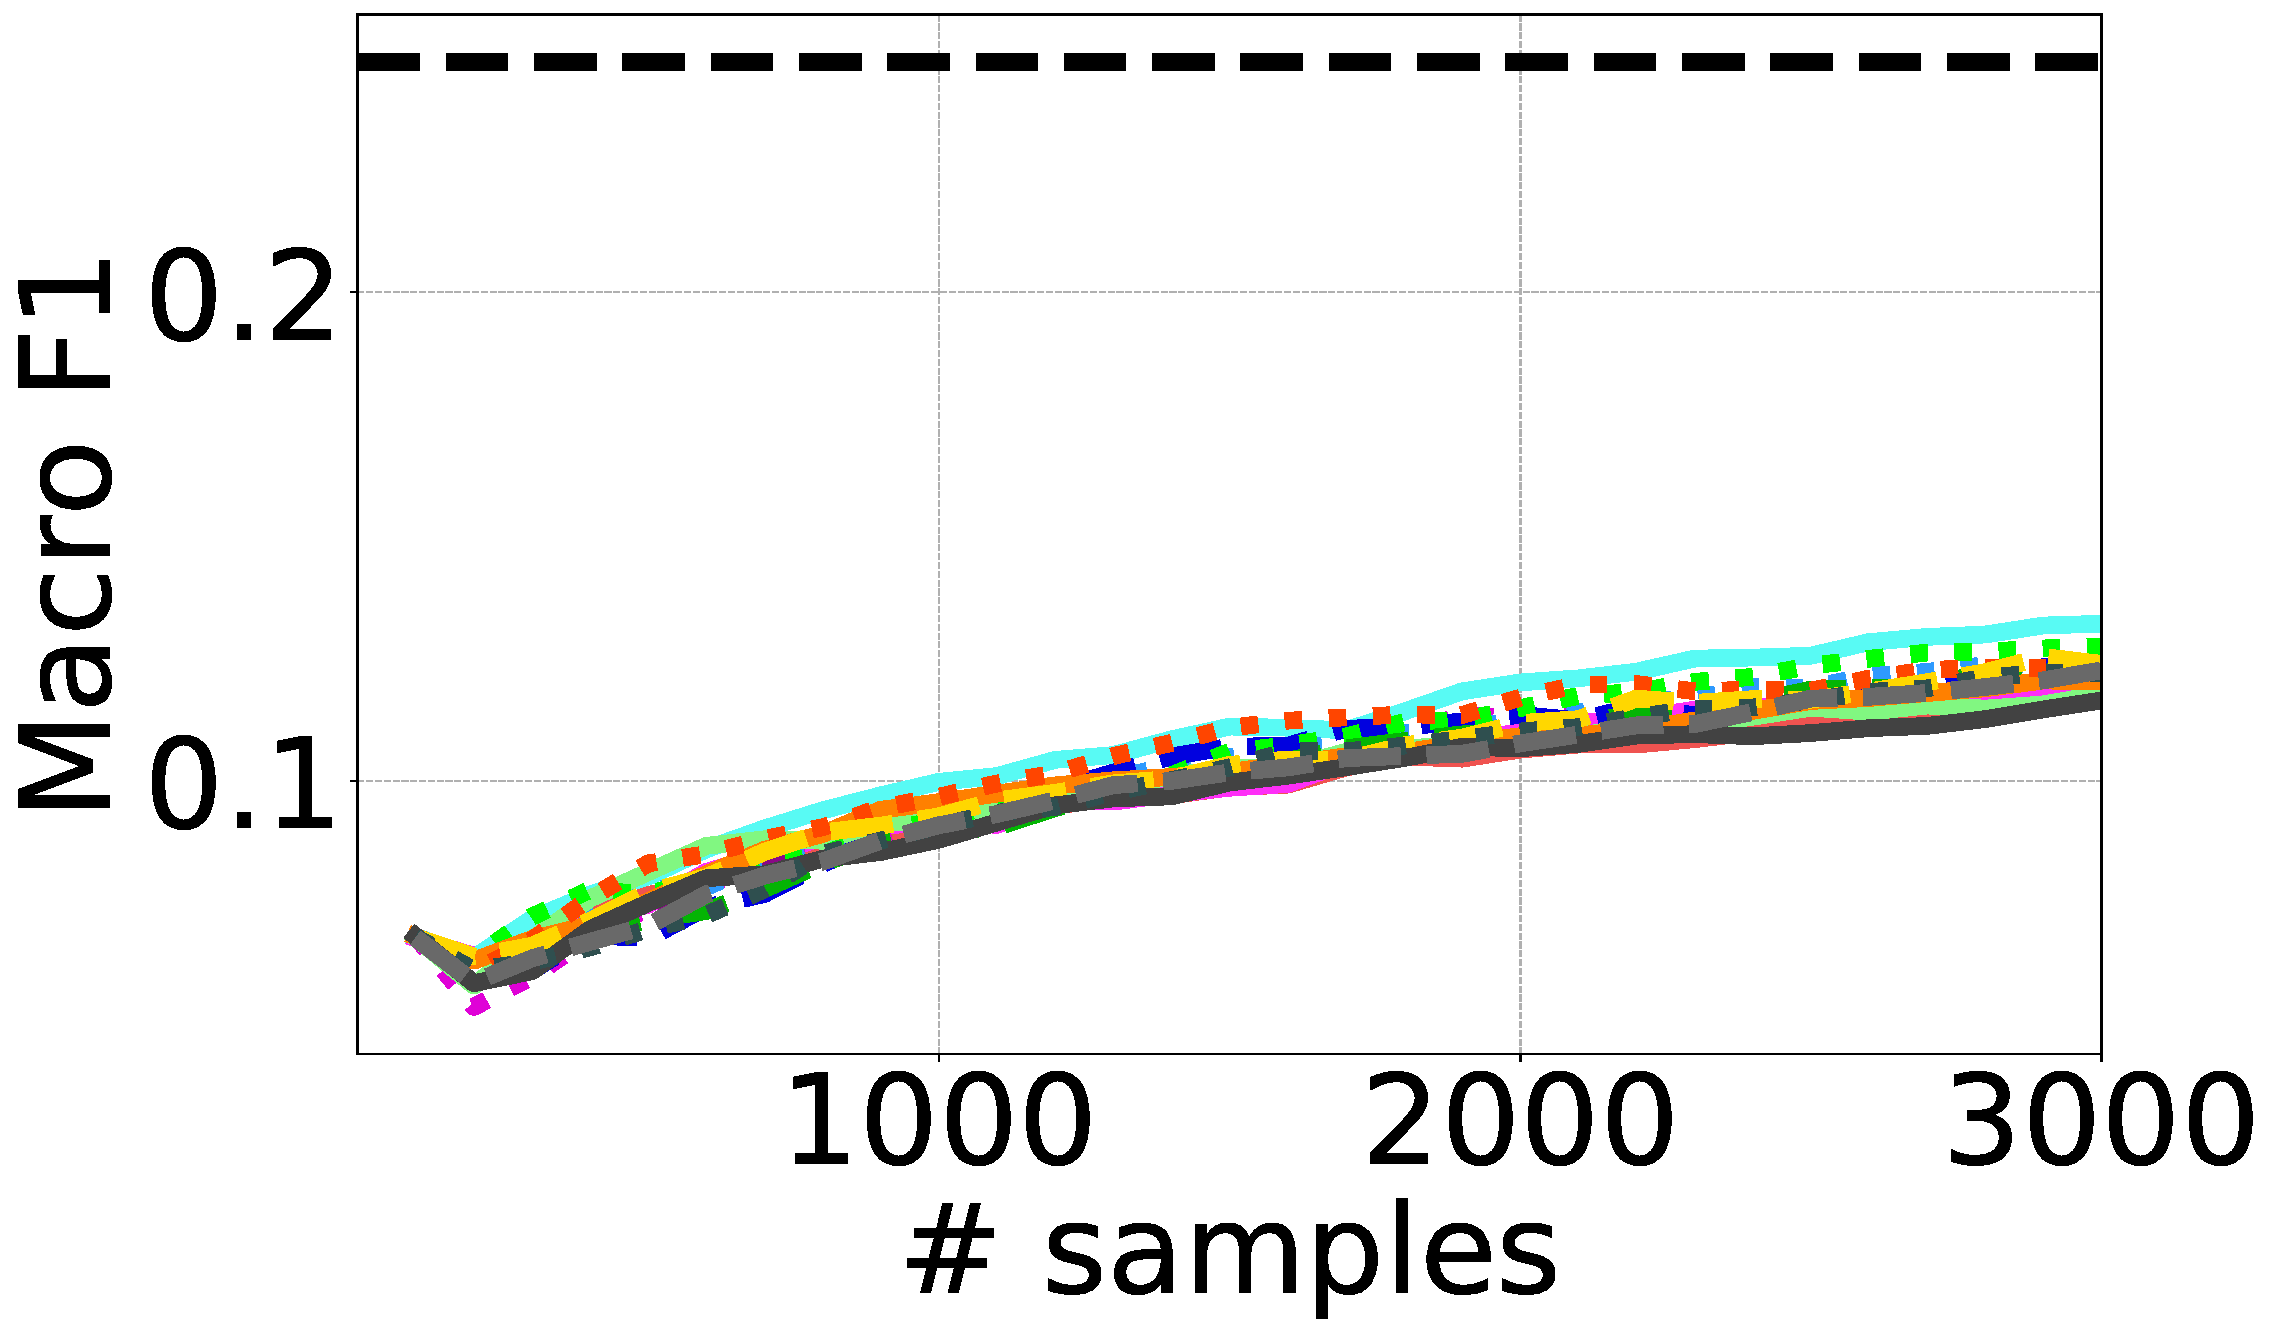
\includegraphics[width=0.24\textwidth]{figs/ft_news_tokenized_acc_all.pdf}}
	
	\end{center}
	\noindent
	\begin{center}
	\subfloat[TNEWS]{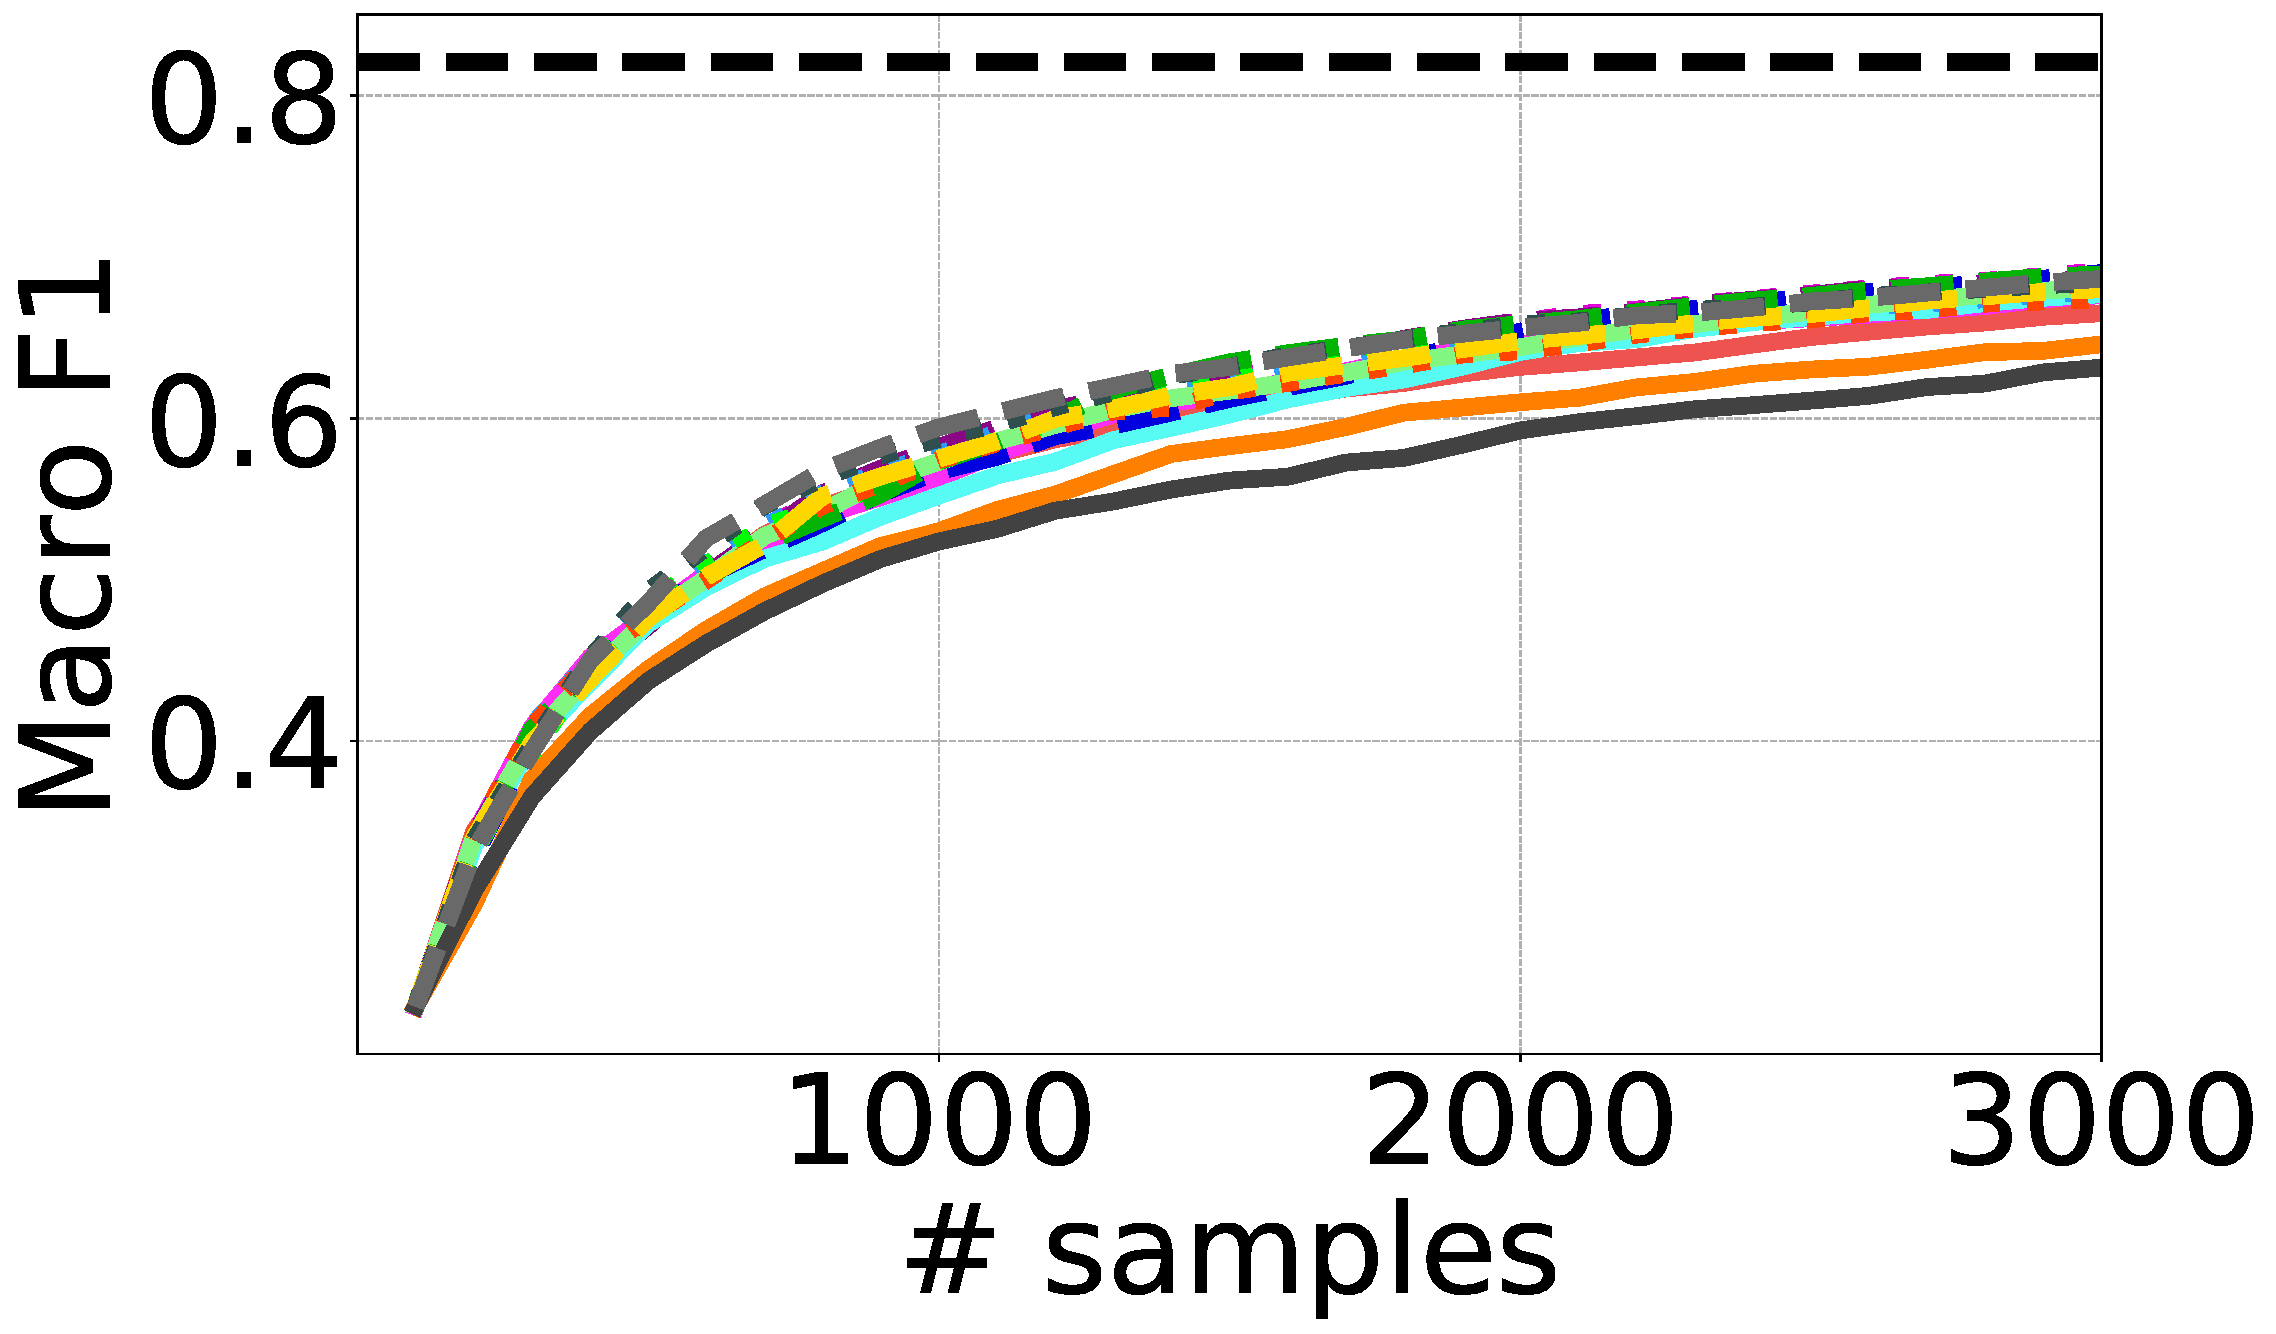
\includegraphics[width=0.24\textwidth]{figs/ft_tnews_tokenized_acc_all.pdf}} % \newline
	\subfloat[GCS]{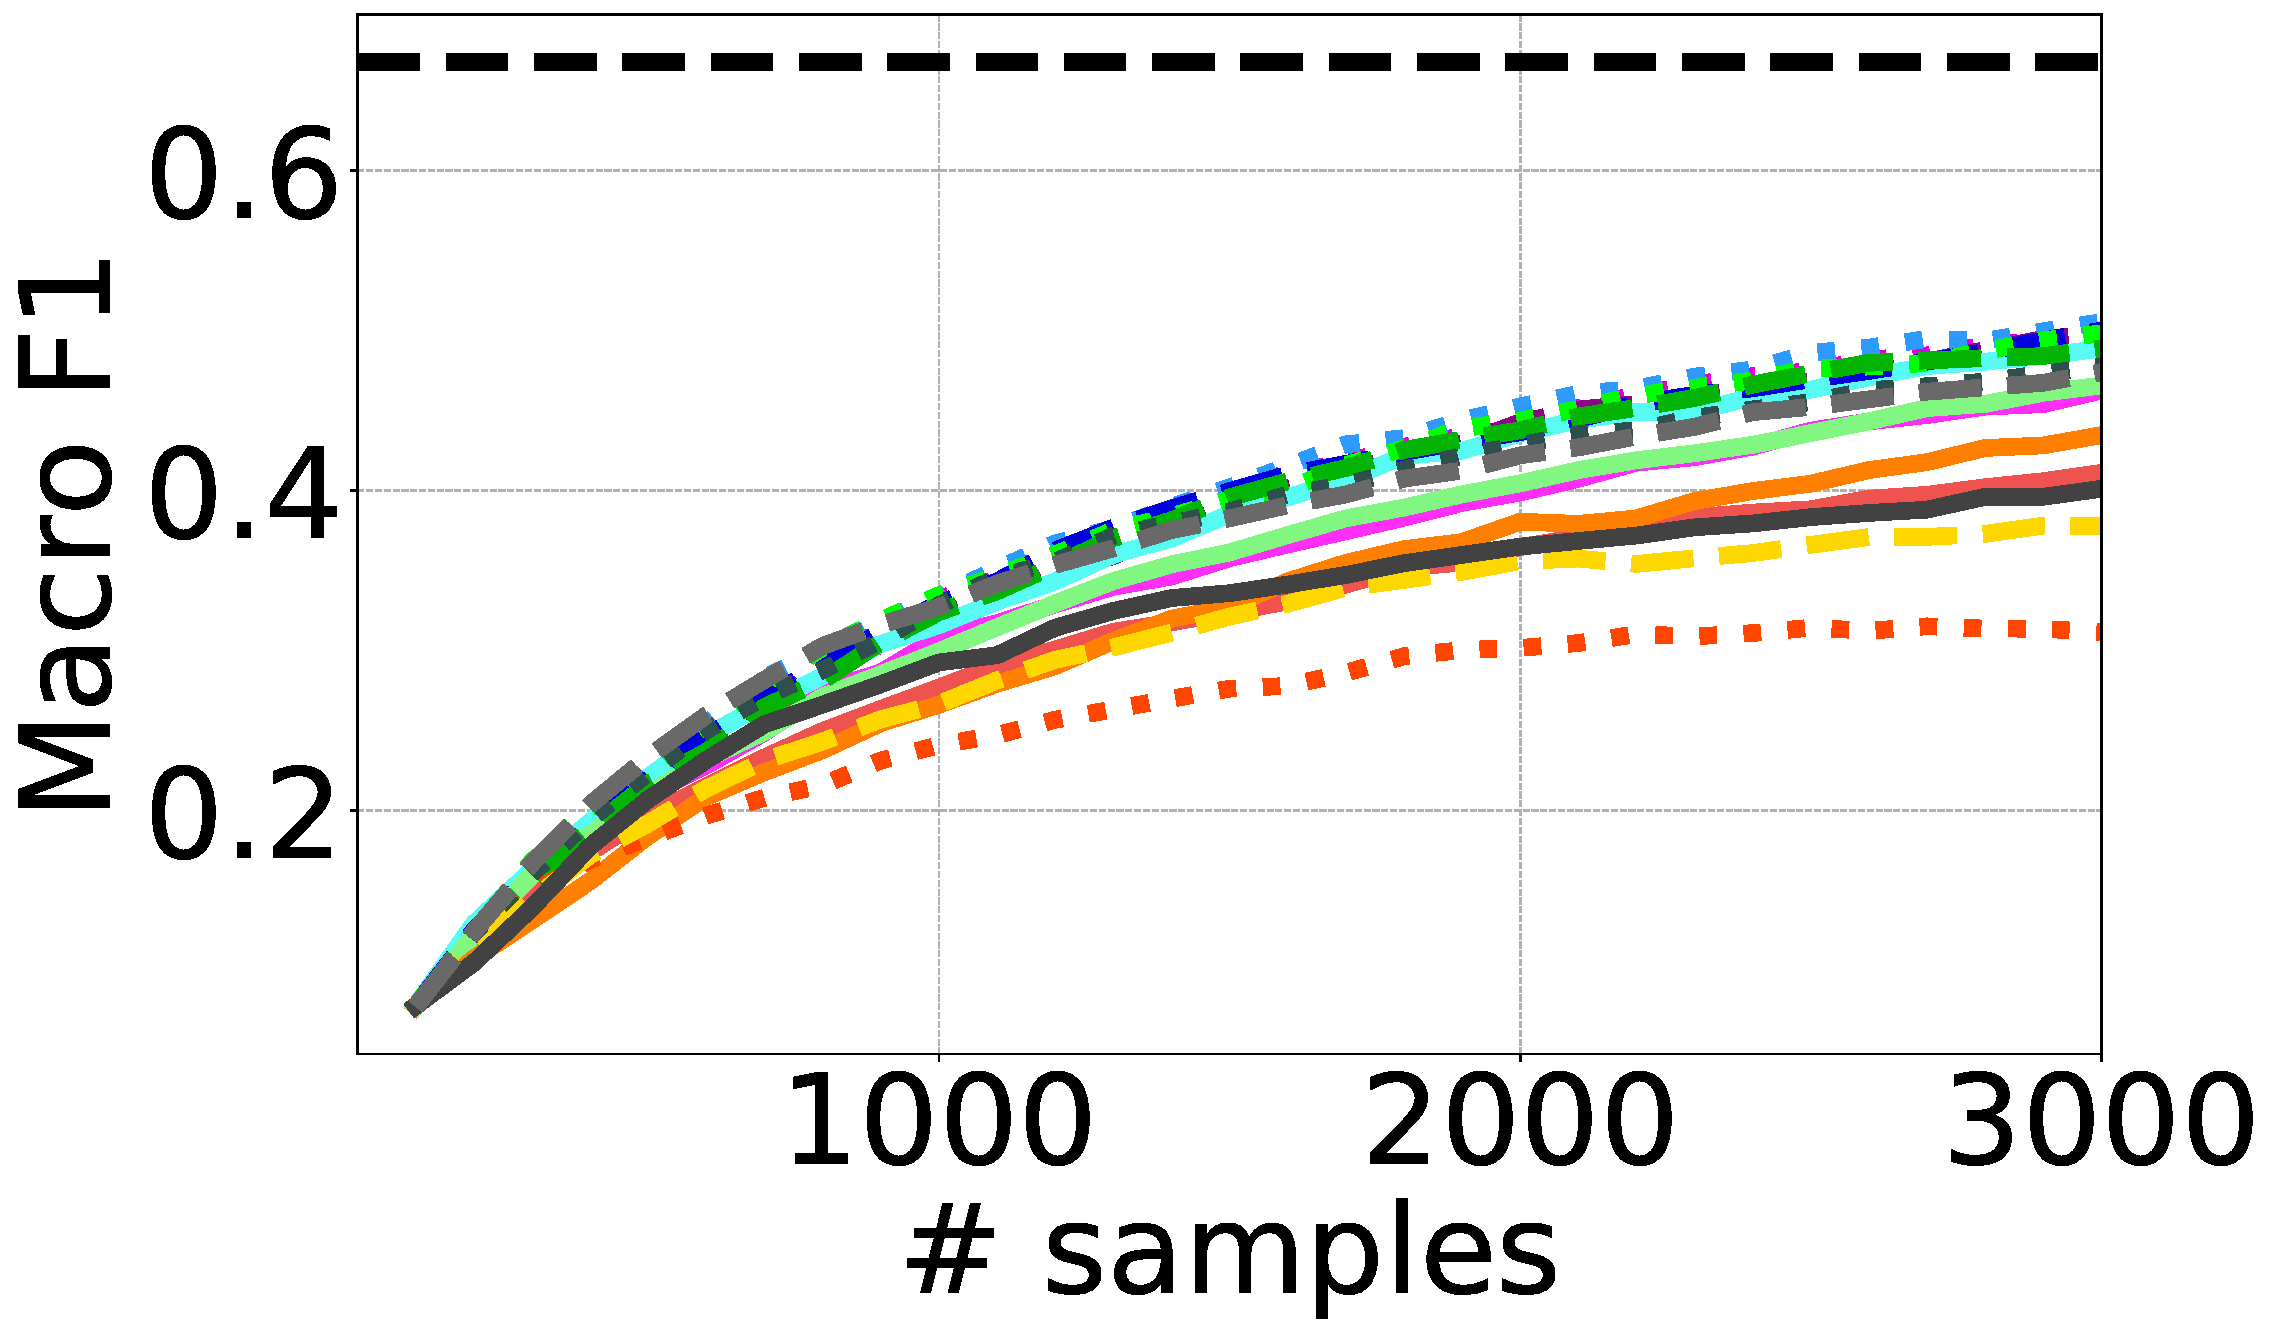
\includegraphics[width=0.24\textwidth]{figs/ft_yanjing_tokenized_acc_all.pdf}}
	\end{center}
	\noindent
\begin{center}
	\subfloat[Biomedical]{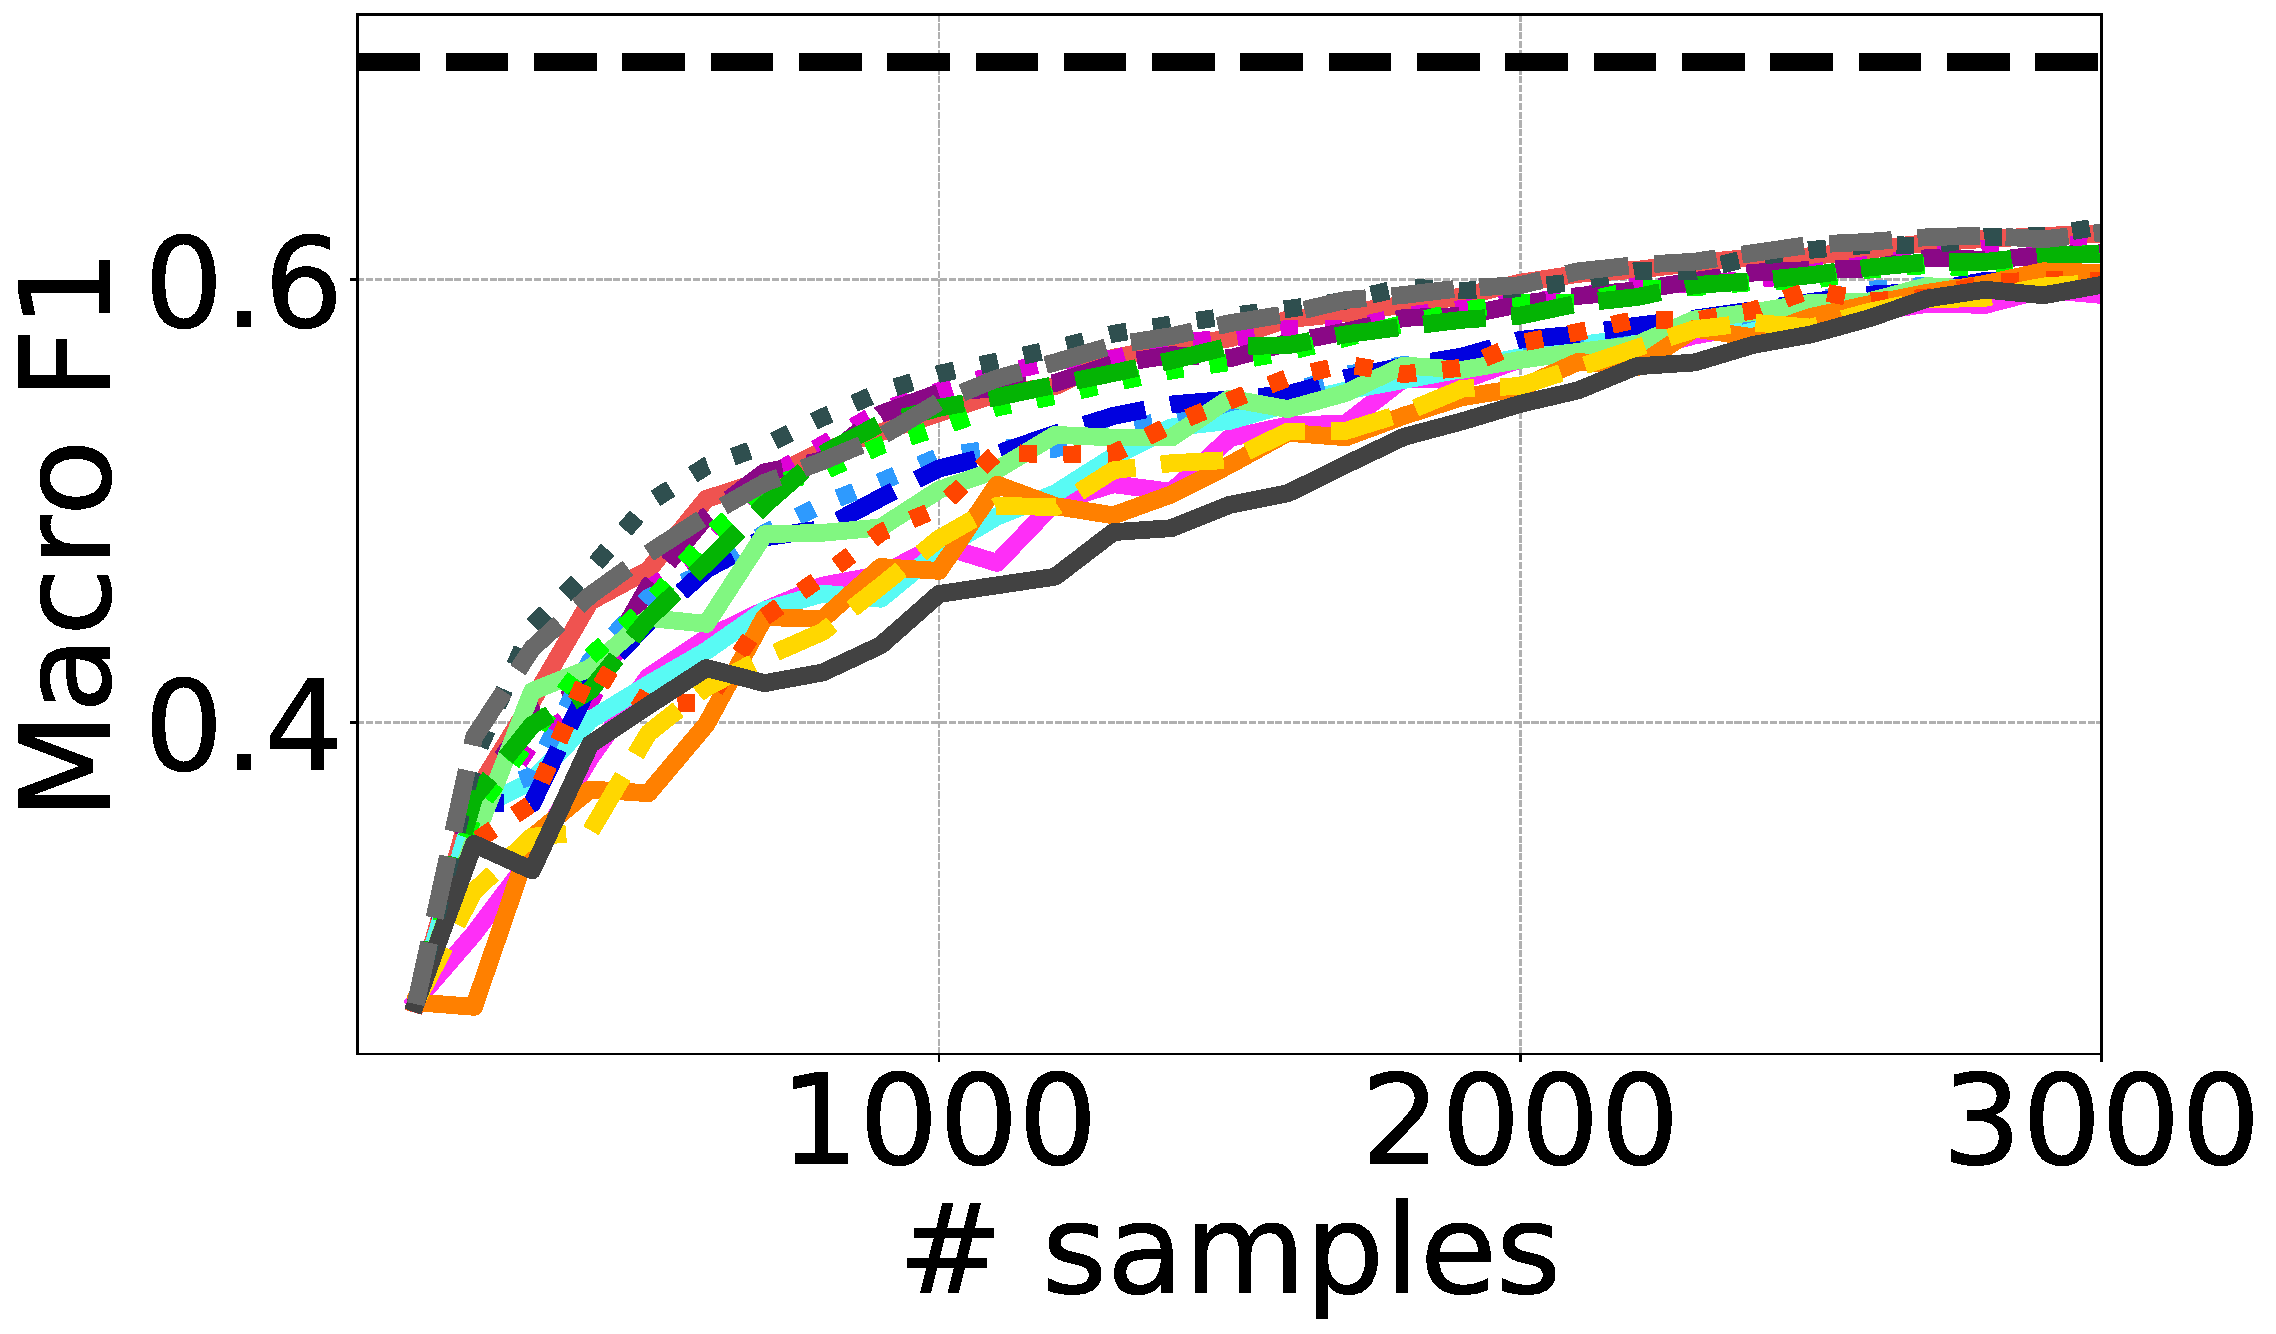
\includegraphics[width=0.24\textwidth]{figs/ft_Biomedical_tokenized_acc_all.pdf}} % \newline
	%\subfloat[StackOverflow]{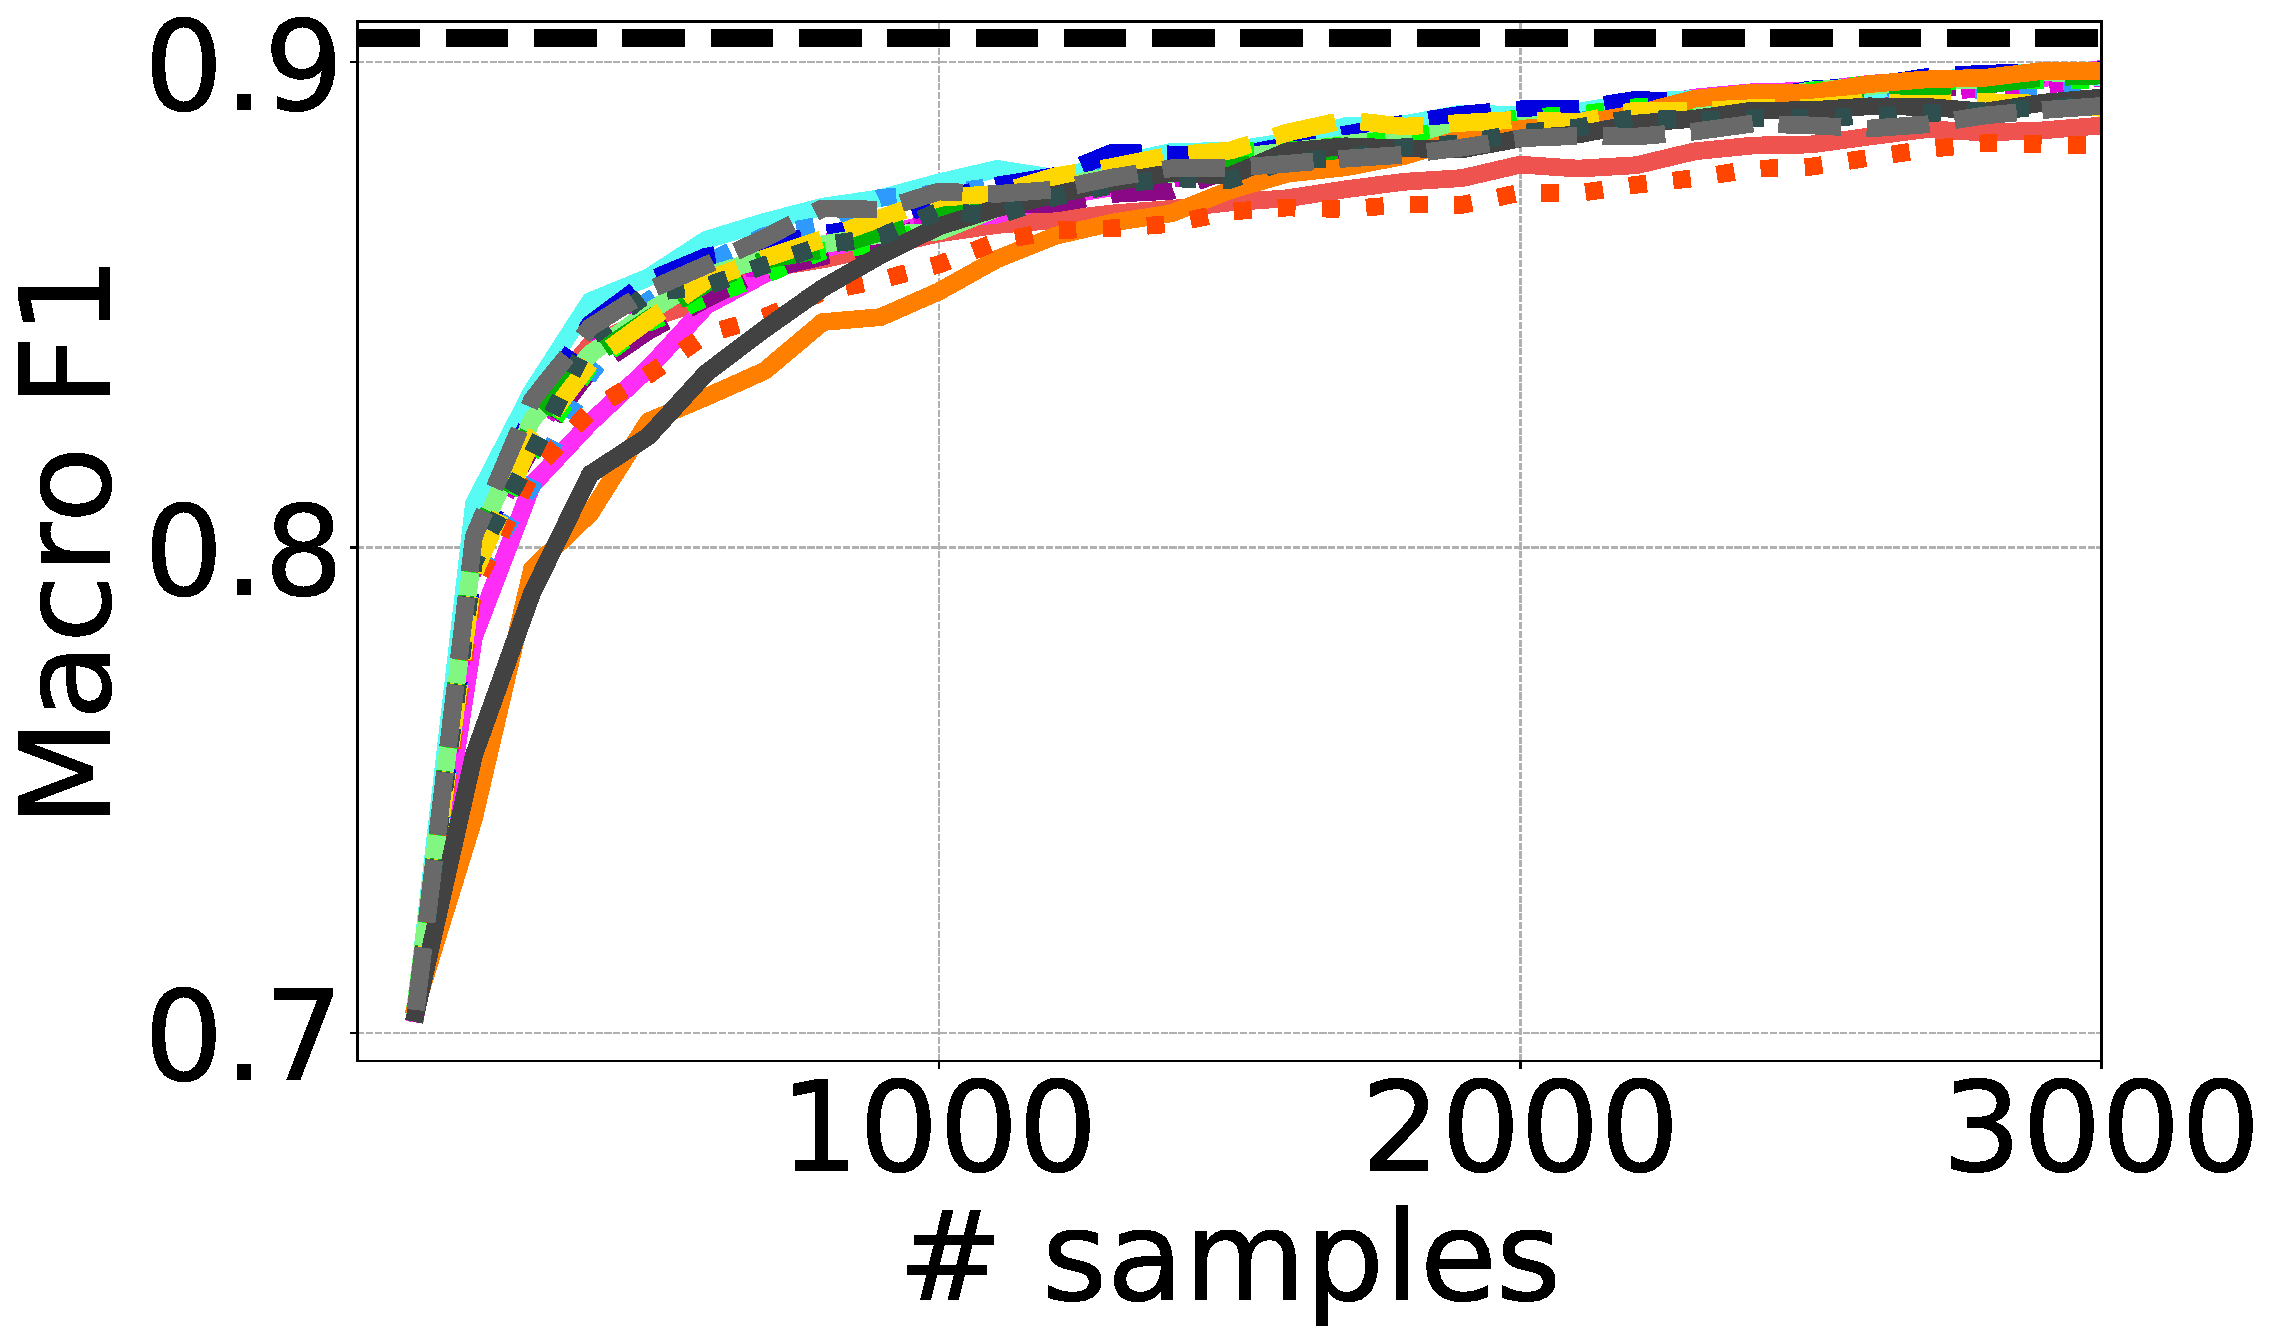
\includegraphics[width=0.24\textwidth]{figs/ft_SO_tokenized_acc_all.pdf}}
	\subfloat[Emoji]{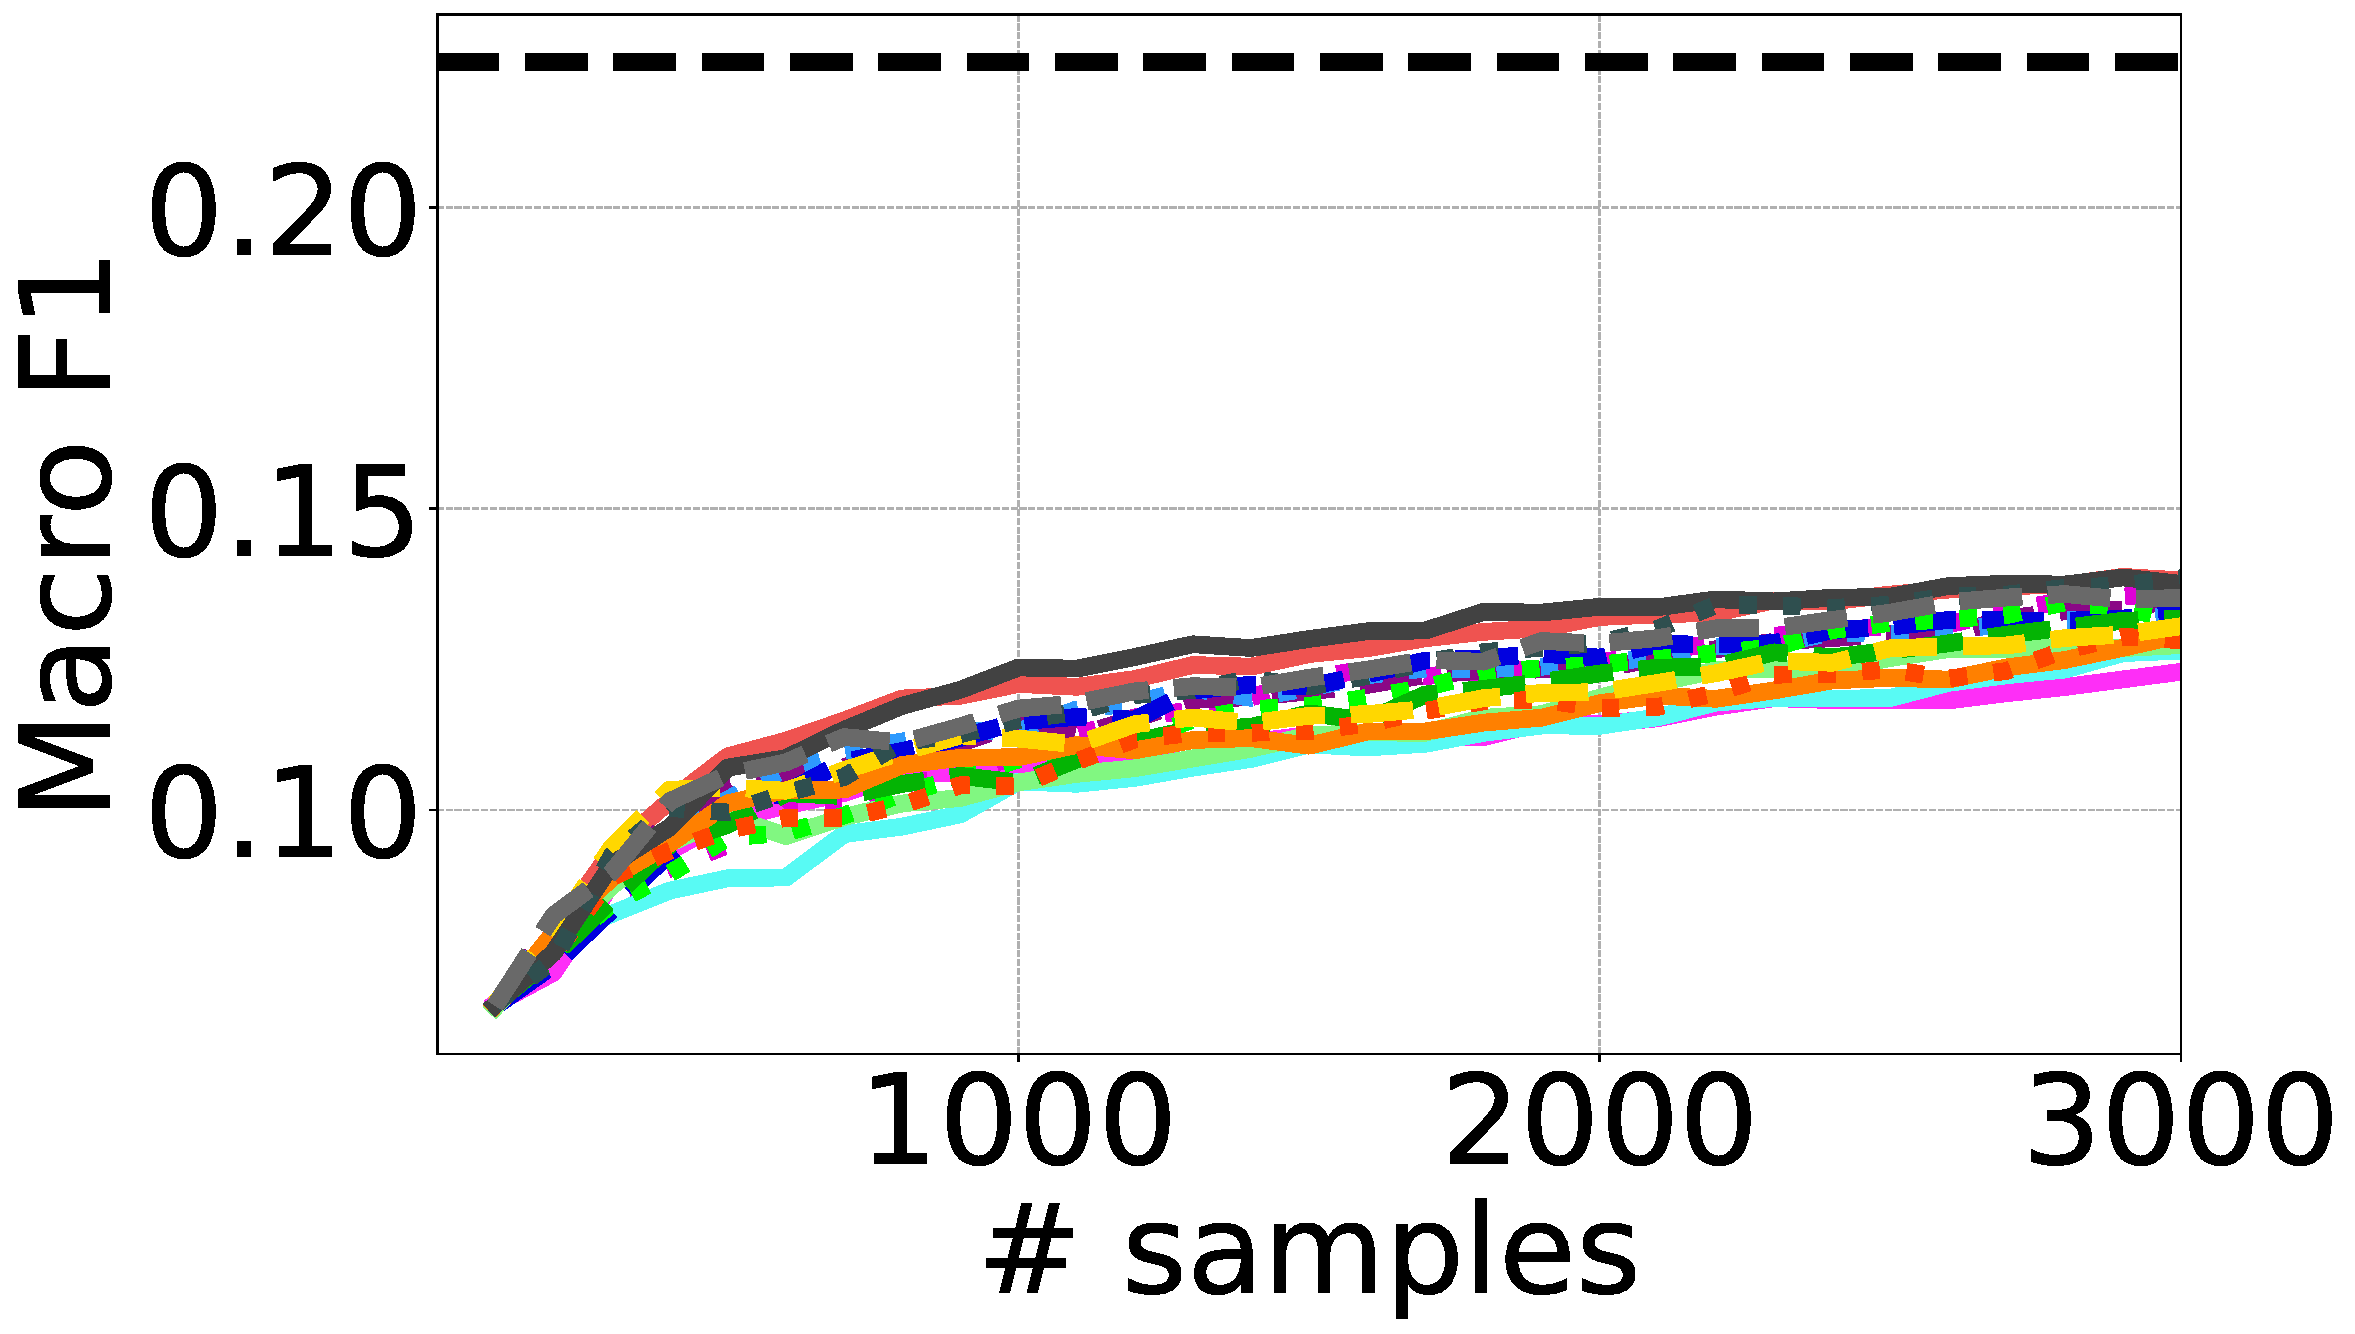
\includegraphics[width=0.24\textwidth]{figs/ft_emoji_tokenized_acc_all.pdf}}
\end{center}
\noindent
\begin{center}
	\subfloat[SearchSnippets]{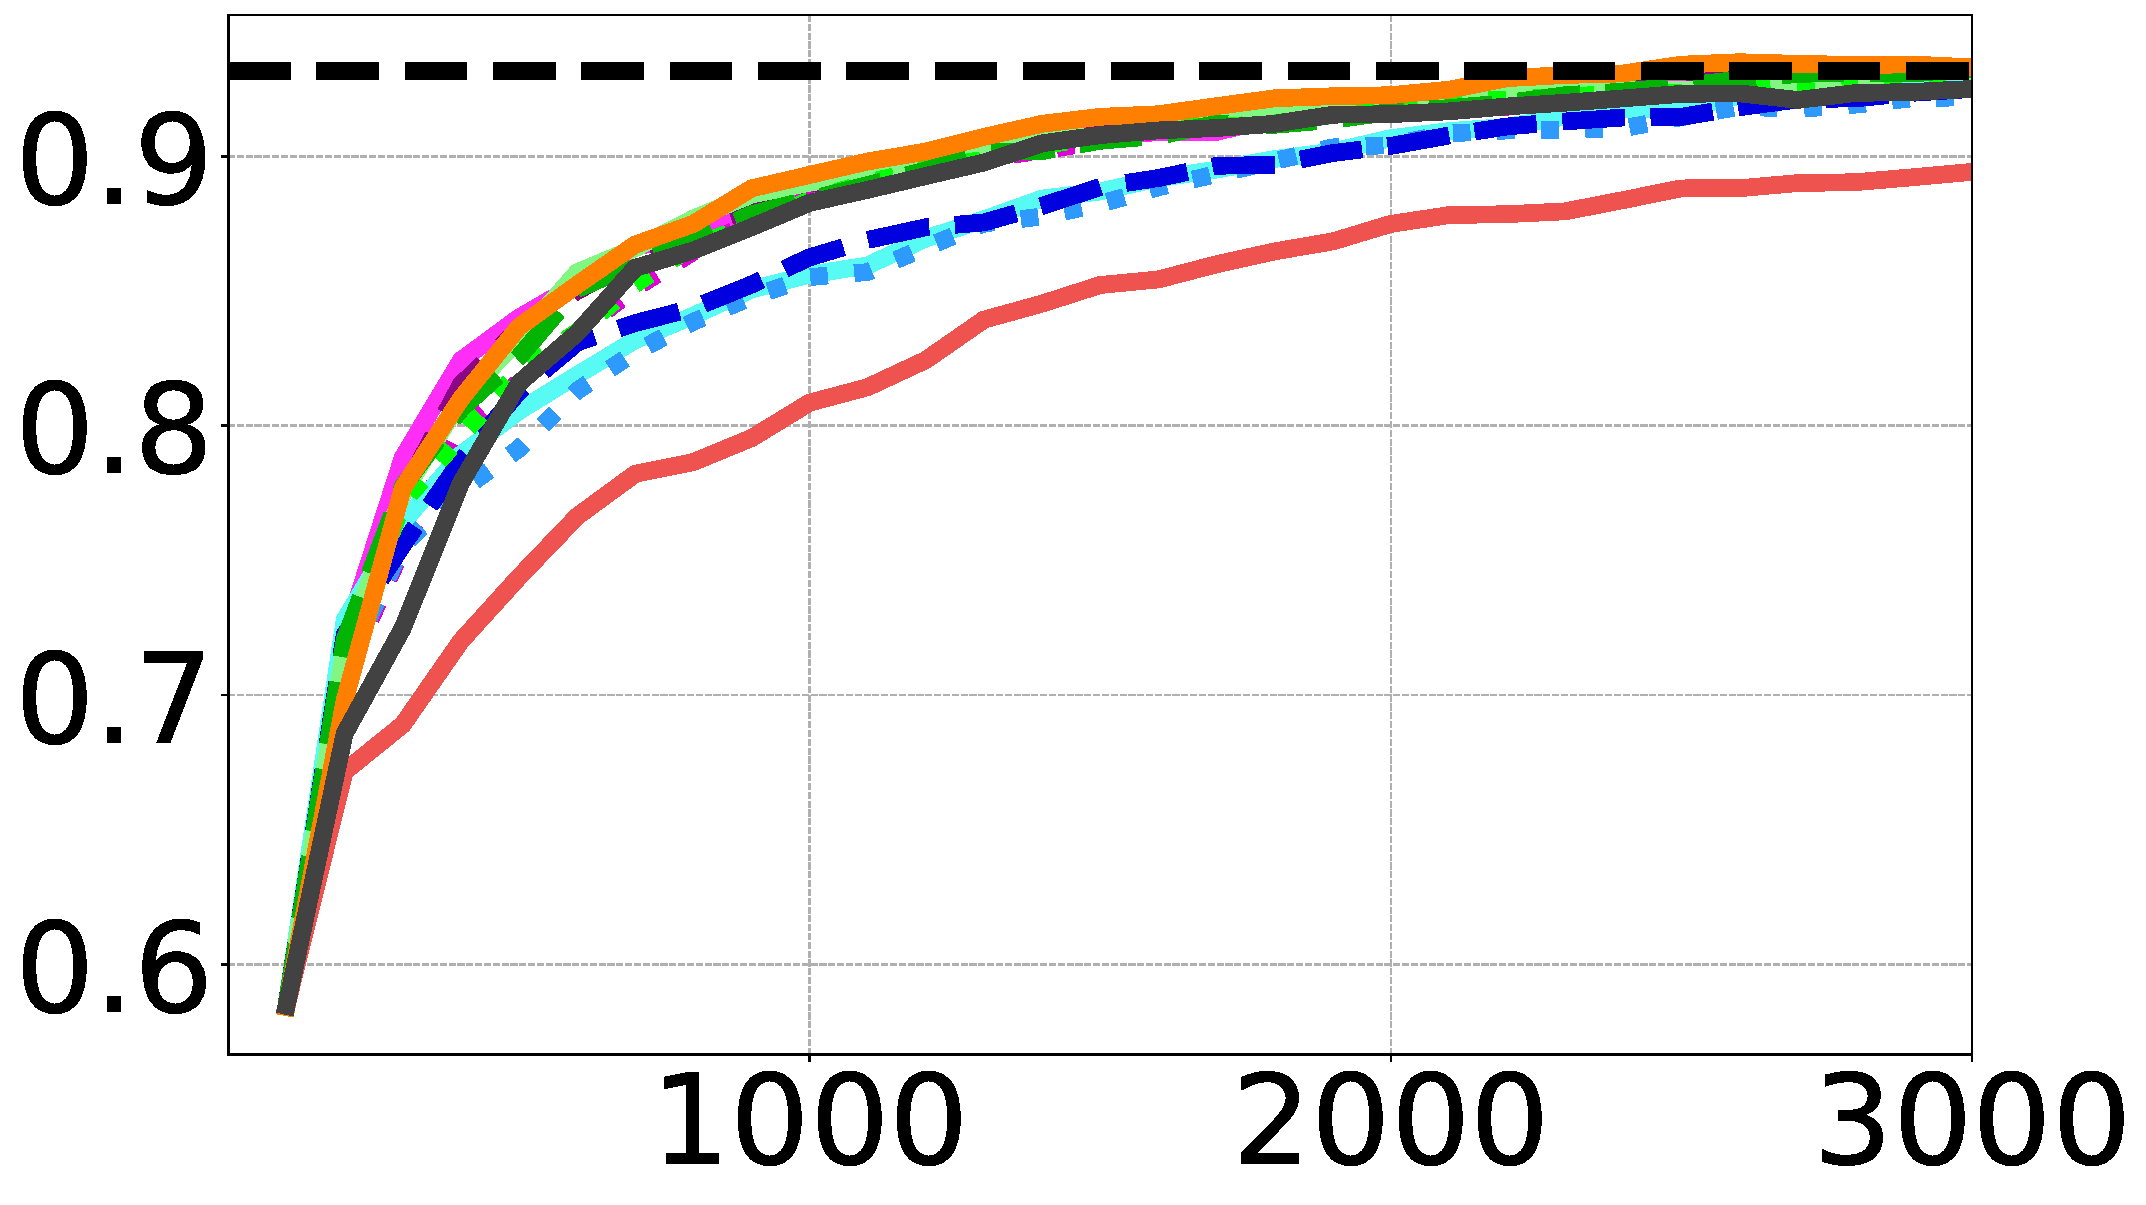
\includegraphics[width=0.24\textwidth]{figs/ft_SearchSnippets_tokenized_acc_all.pdf}}
	\subfloat[Book]{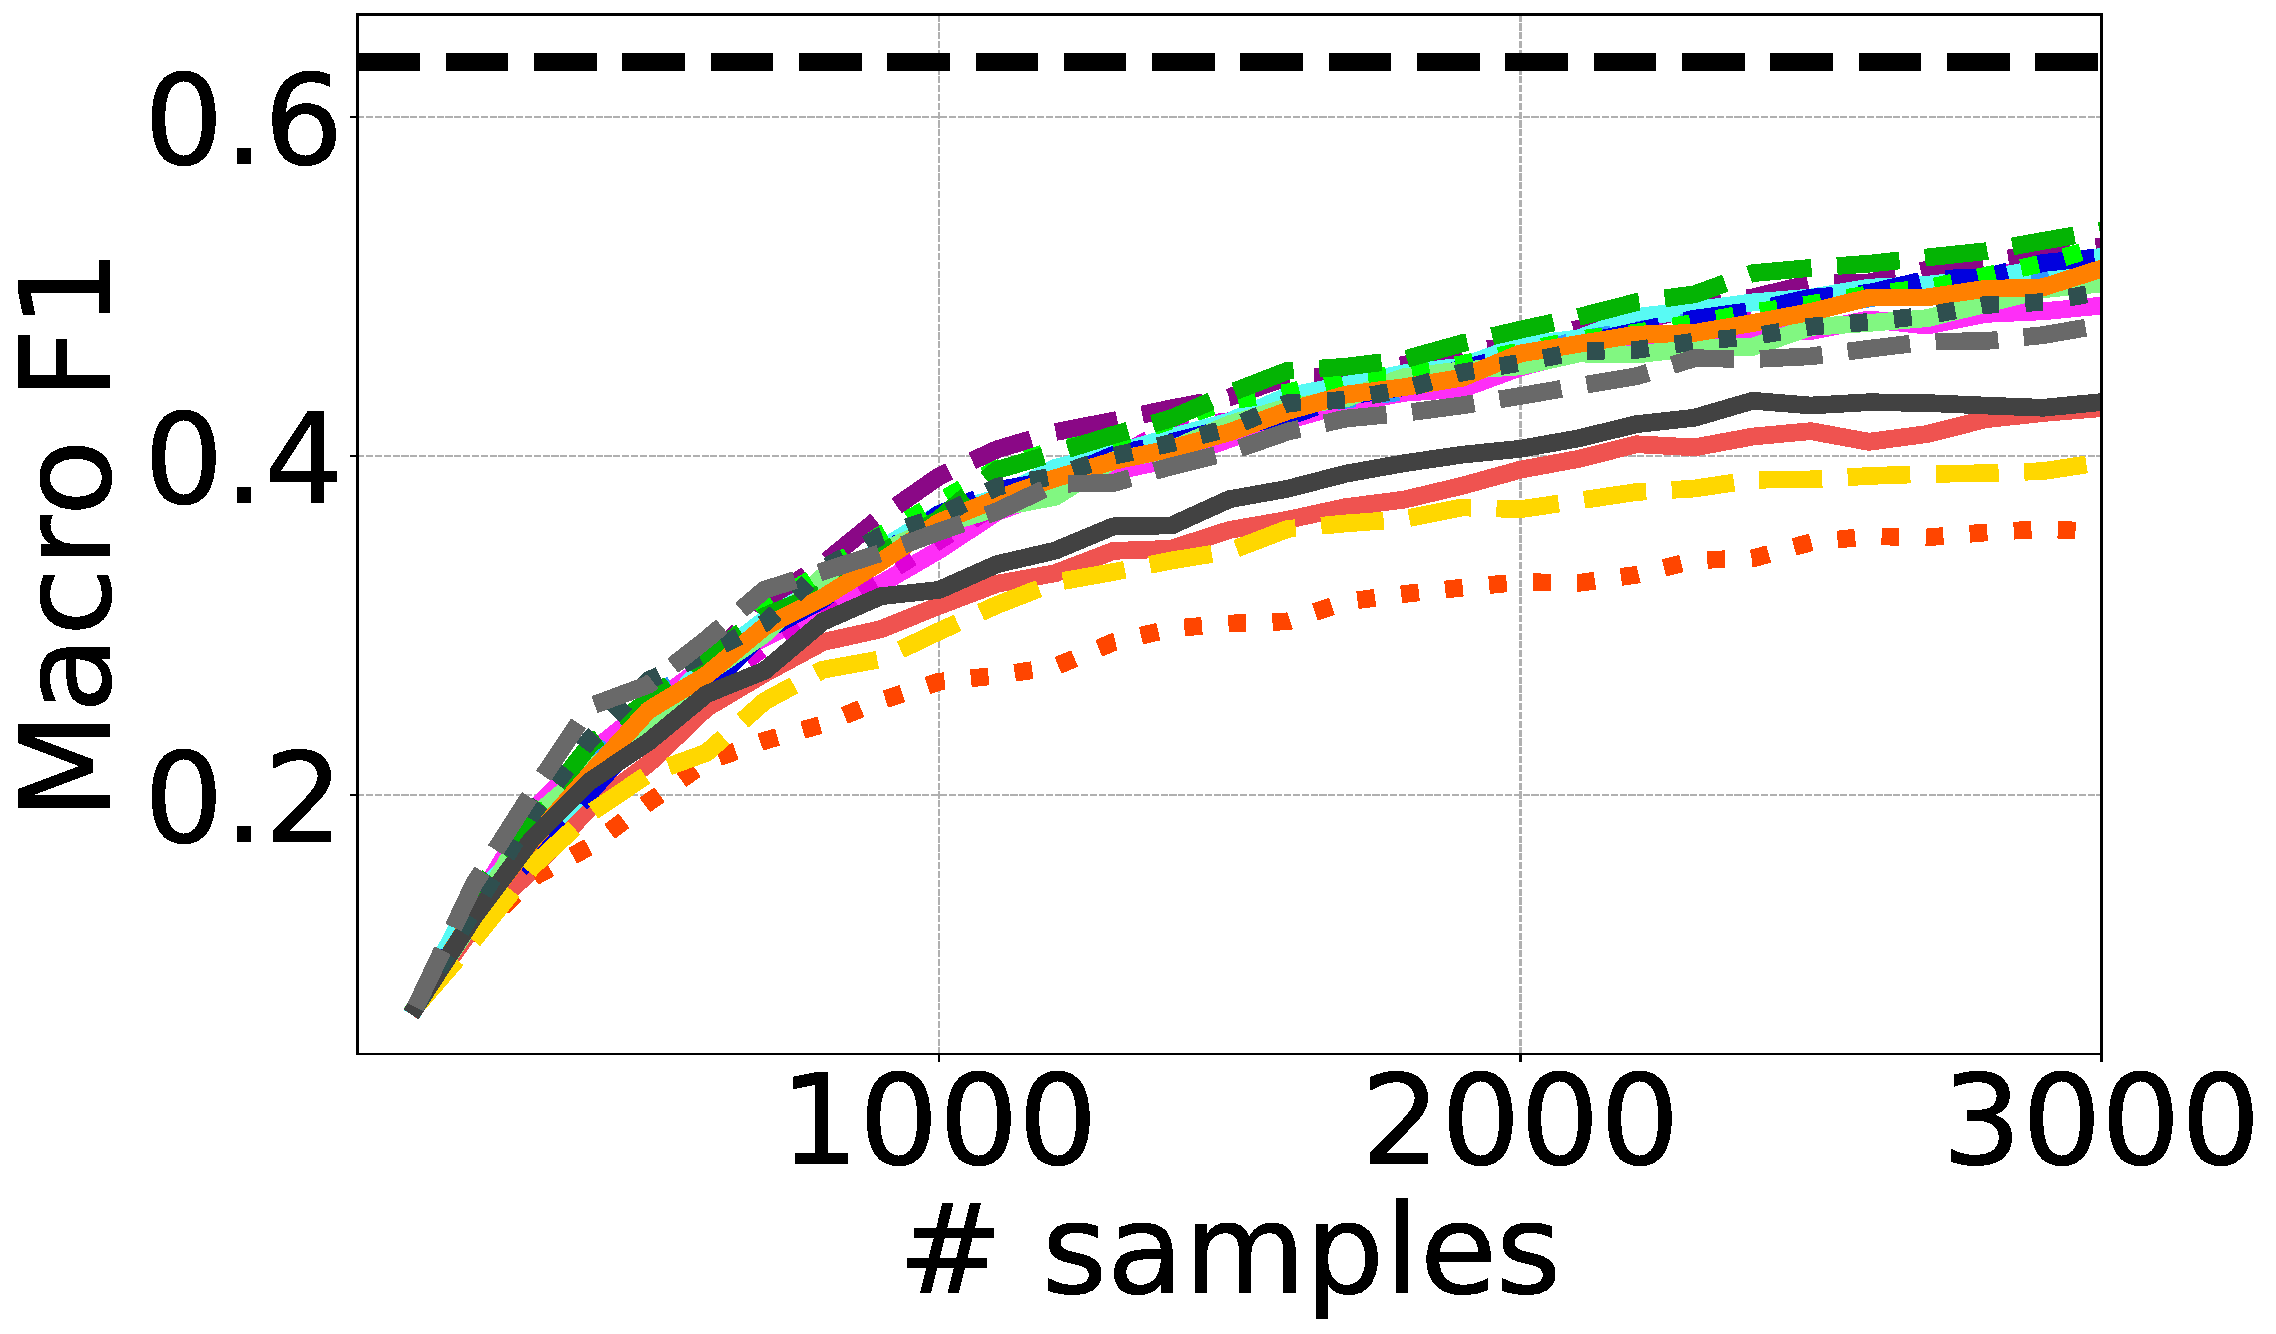
\includegraphics[width=0.24\textwidth]{figs/ft_book_tokenized_acc_all.pdf}}
\end{center}
\caption{Macro F1 curve of AL approaches on 8 datasets using fastText}
\label{fig:acc_all}
\end{figure}


\begin{figure}[th!]%[!hbt]
	\noindent
	\begin{center}
		\subfloat[Reuters]{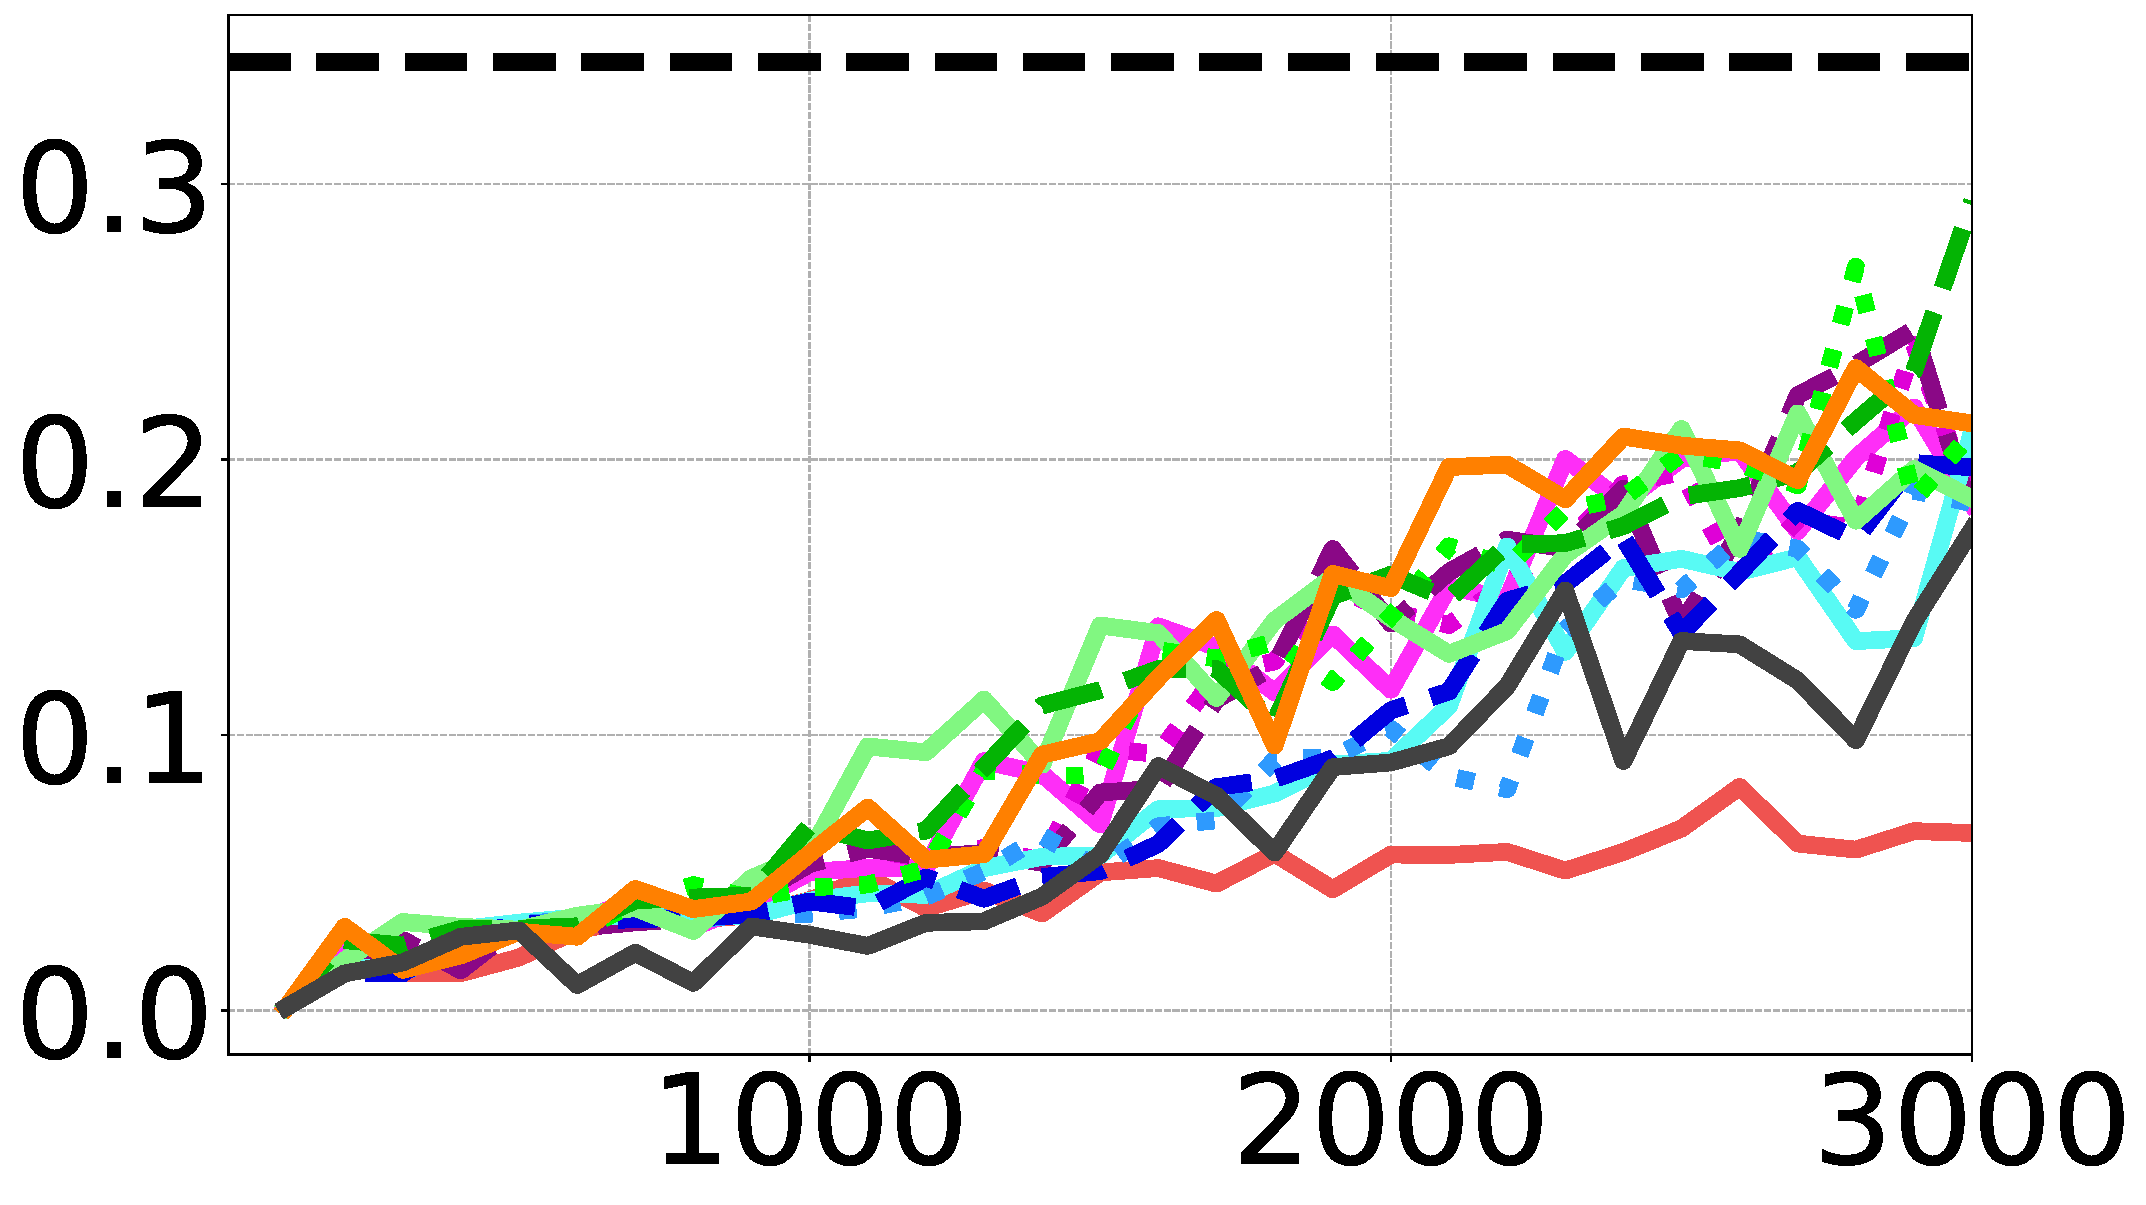
\includegraphics[width=0.24\textwidth]{figs/bert_reuters_acc_all.pdf}}
		\subfloat[SQD]{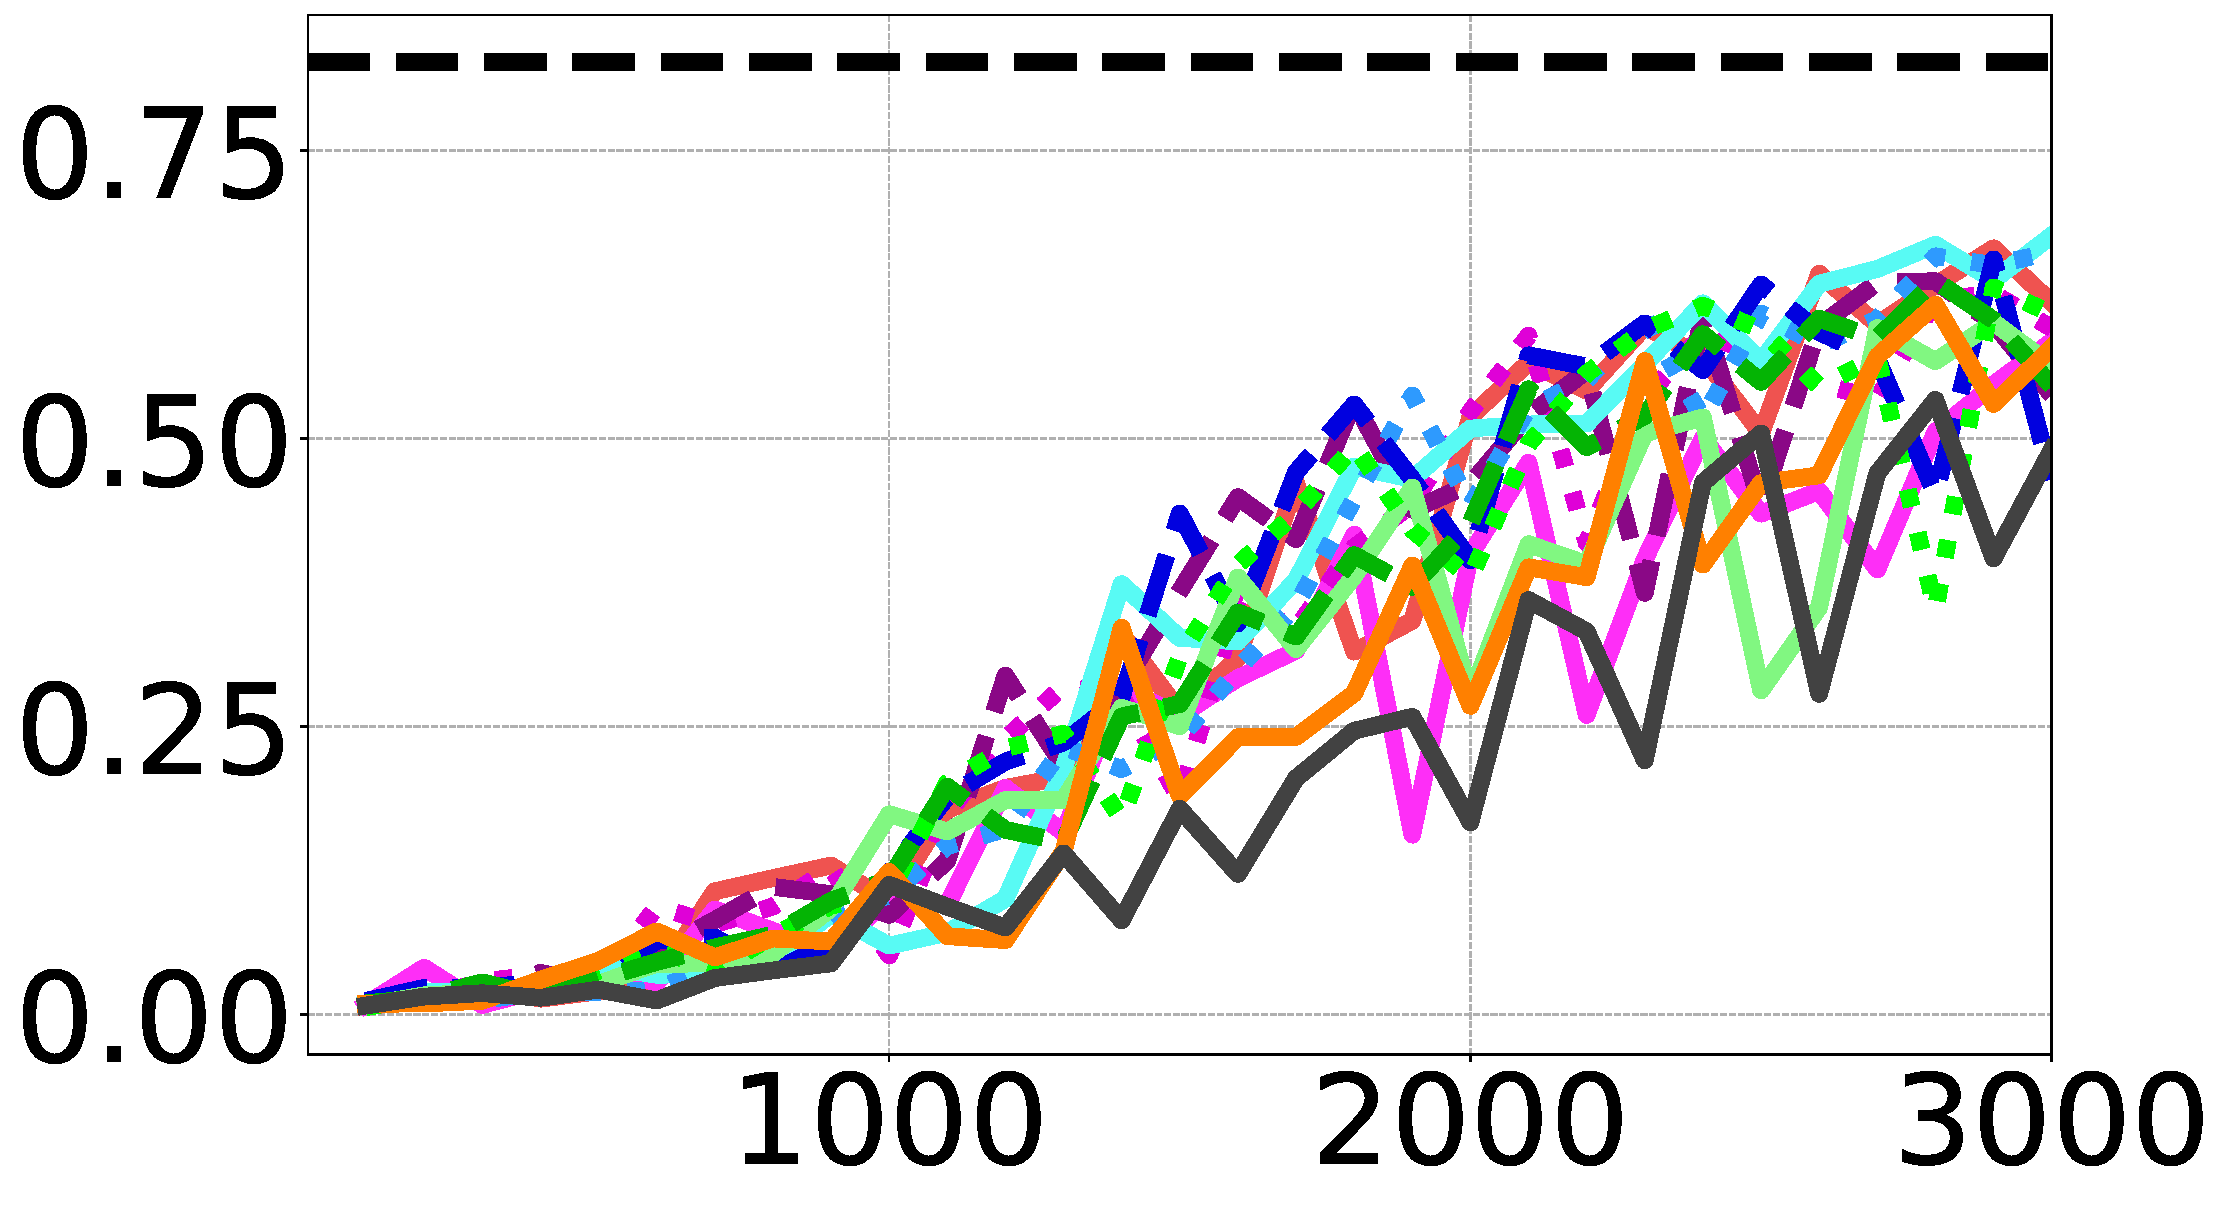
\includegraphics[width=0.24\textwidth]{figs/bert_stack_merge_acc_all.pdf}}
	\end{center}

%	\noindent
%	\begin{center}
%		\subfloat[SQD (5 epochs)]{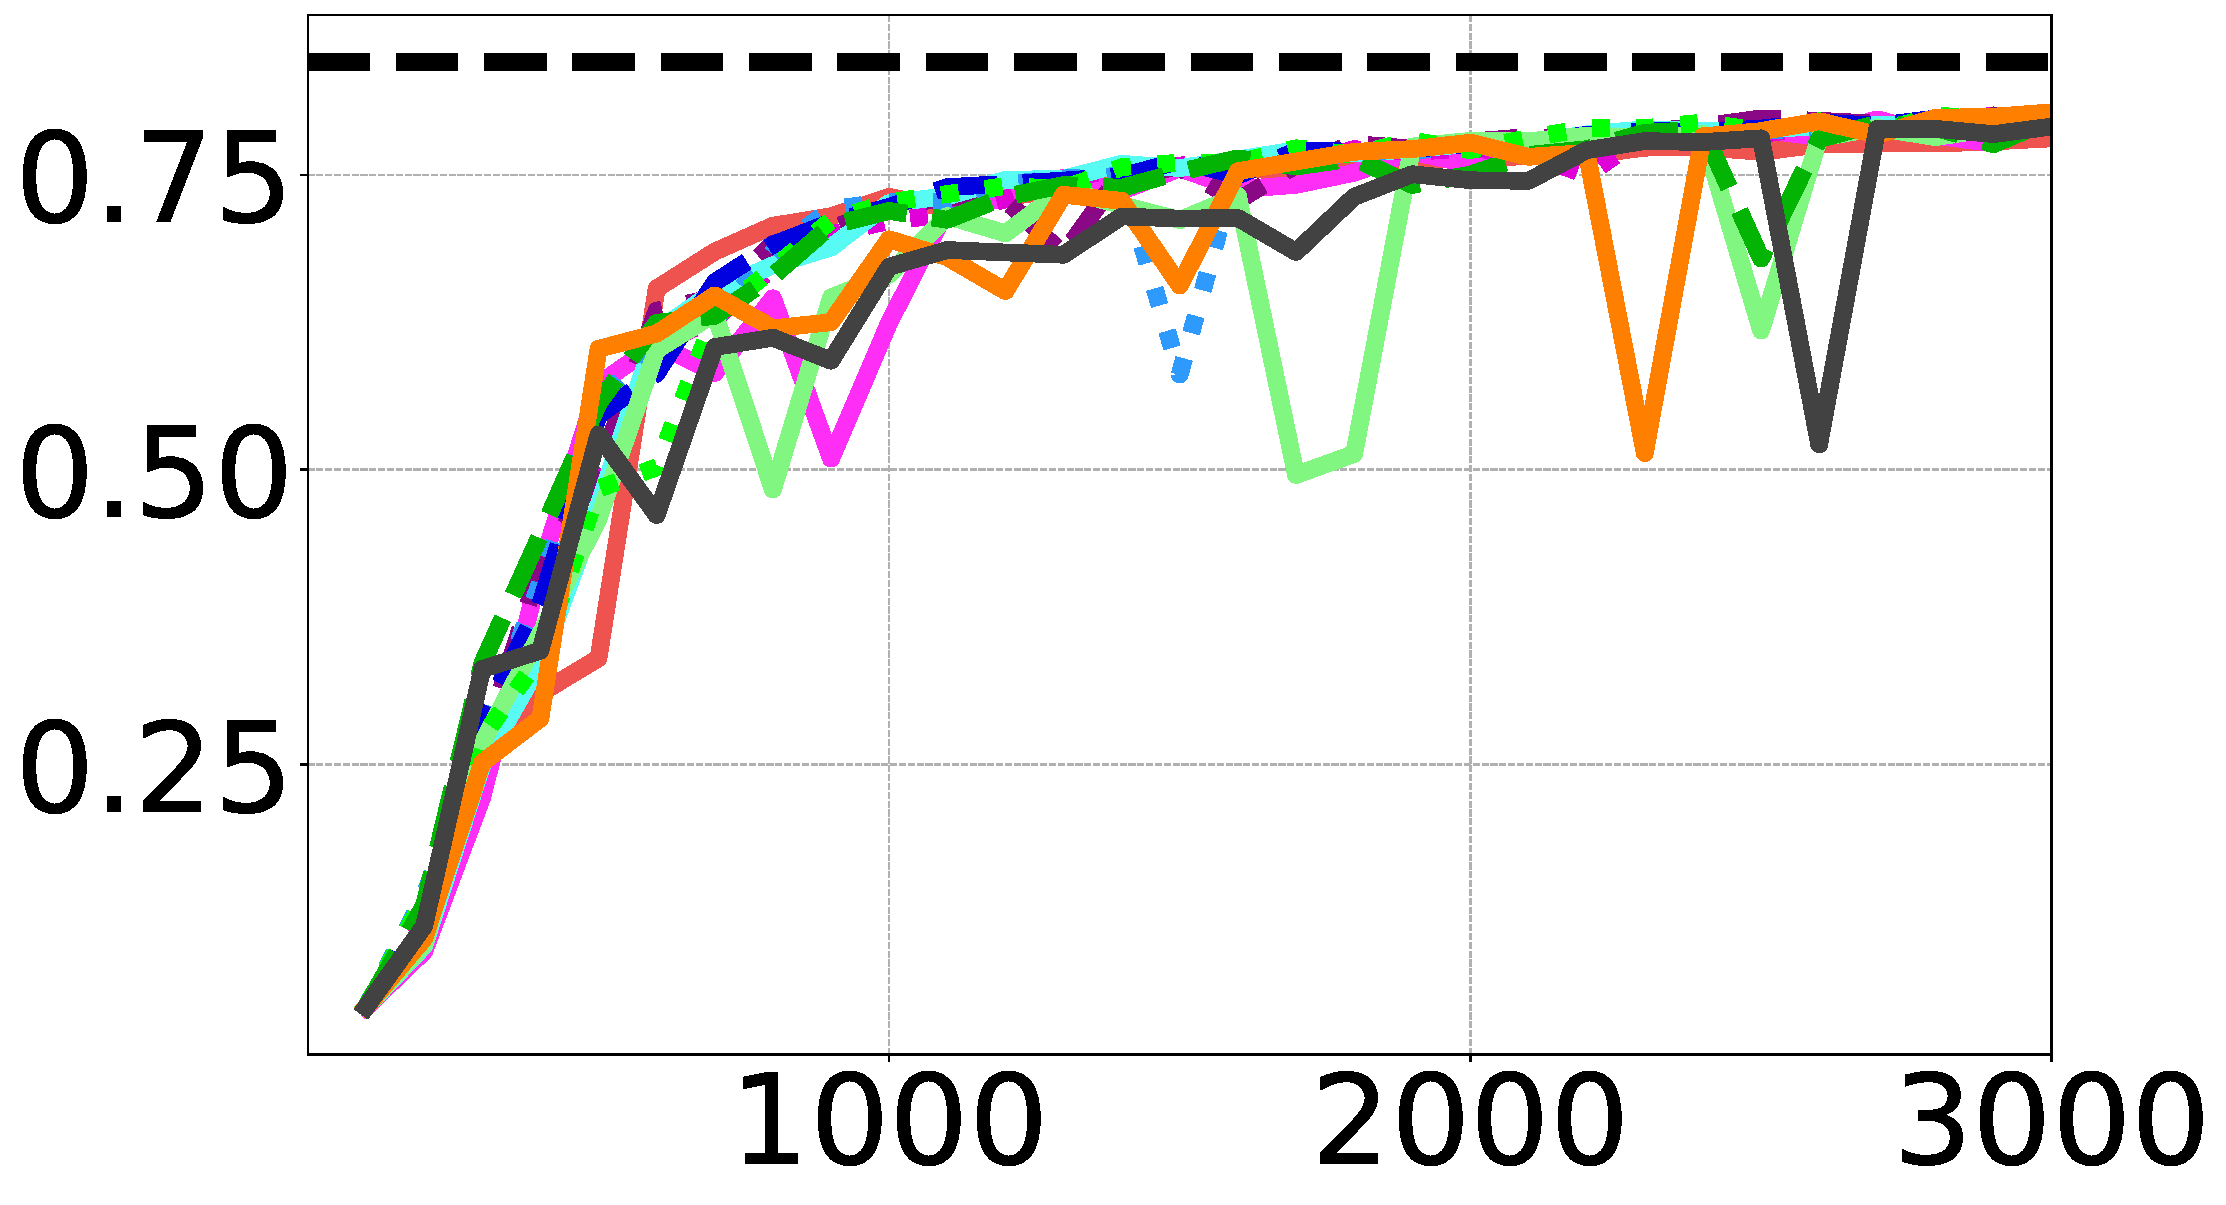
\includegraphics[width=0.24\textwidth]{figs/bert_stack_epoch5_acc_all.pdf}}
%	\end{center}


	\noindent
	\begin{center}
		\subfloat[TNEWS]{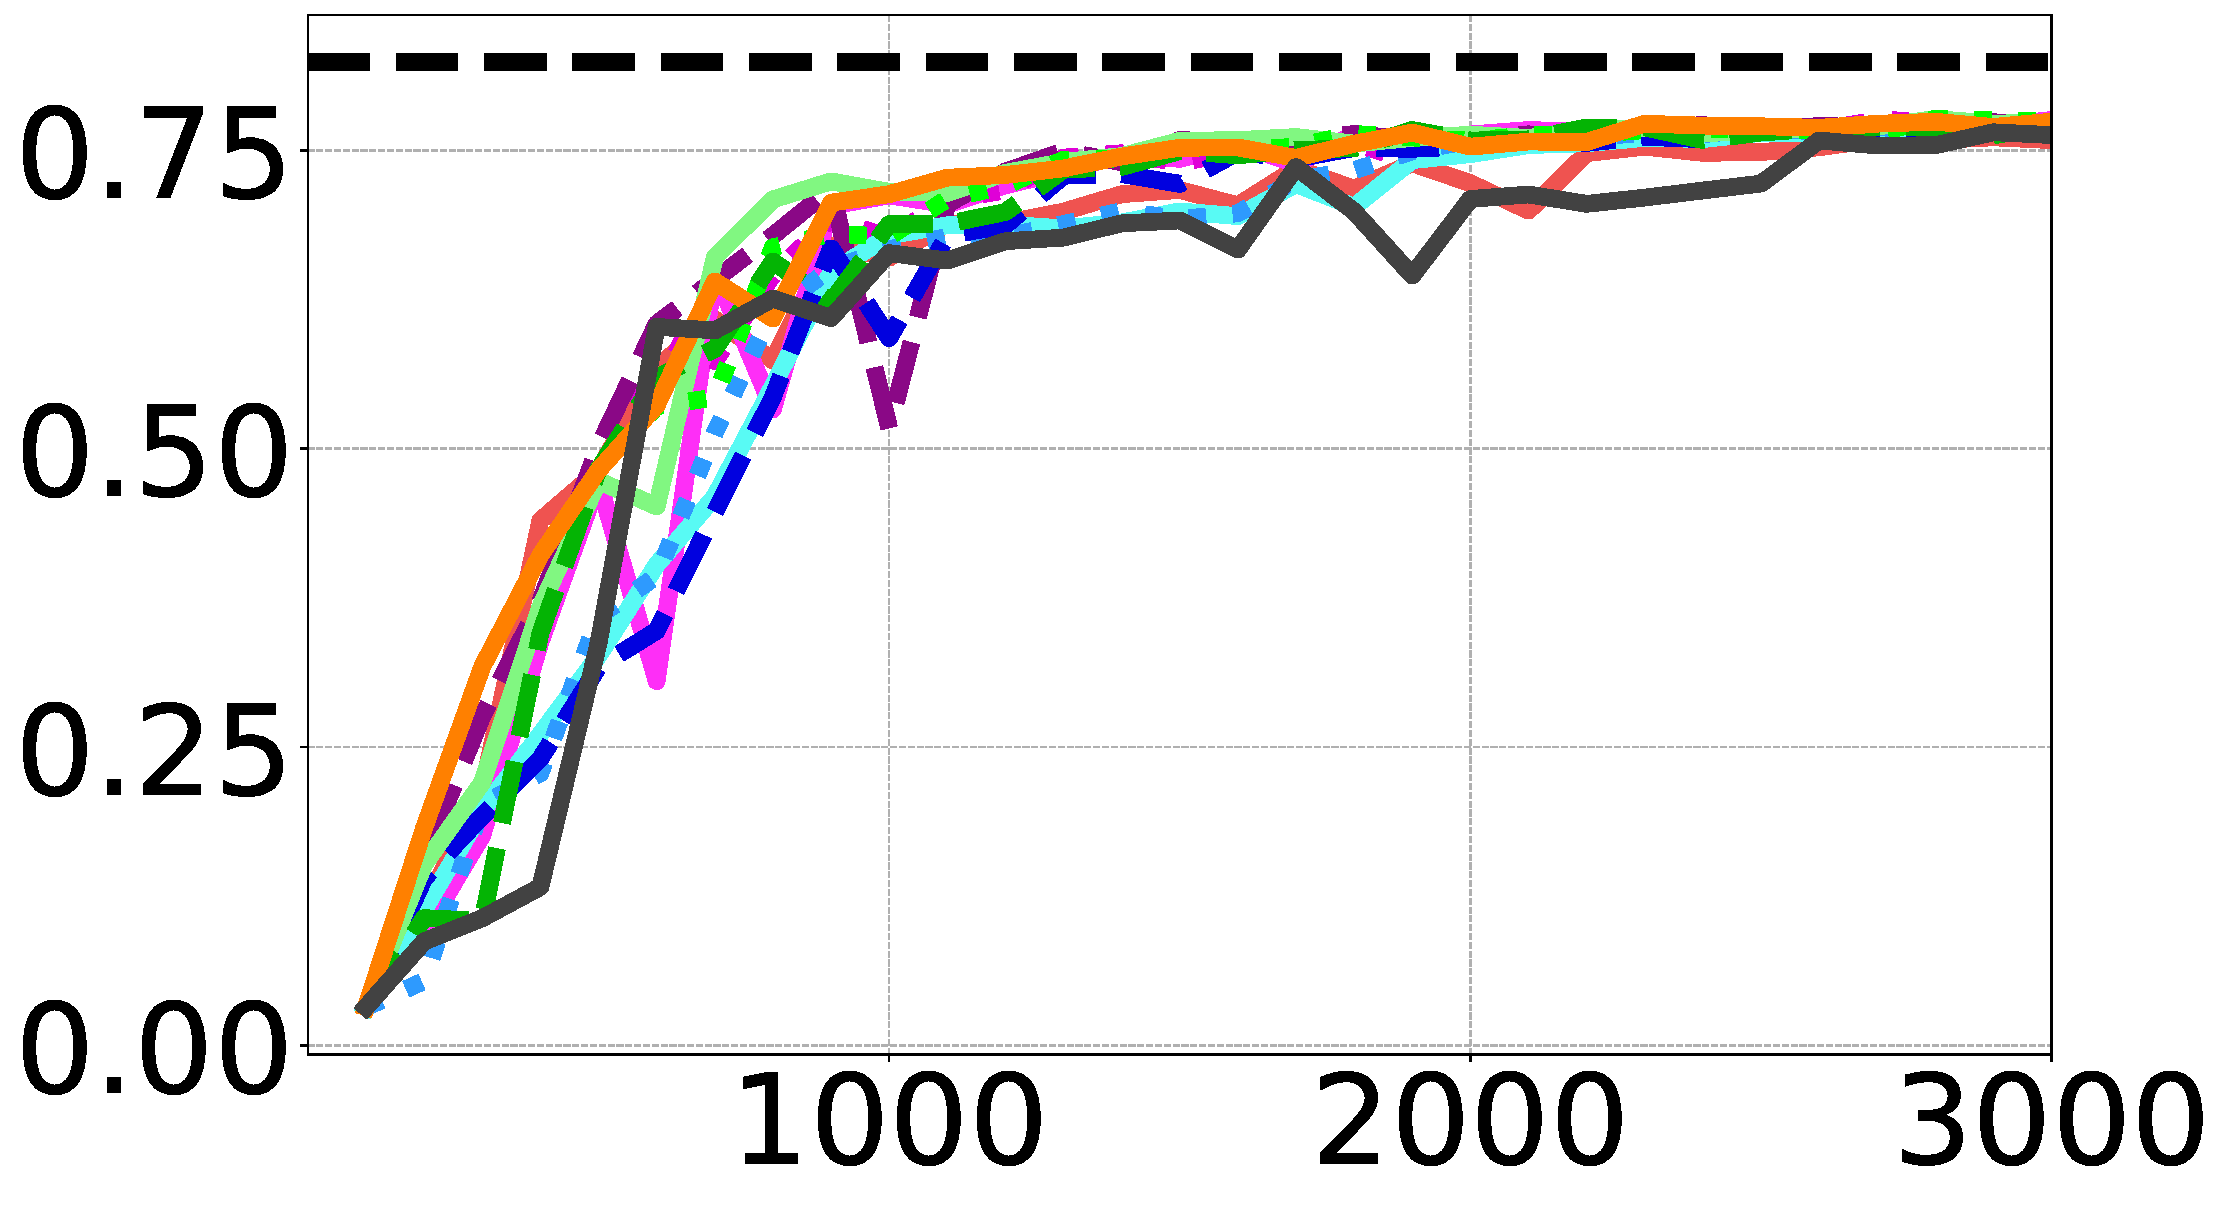
\includegraphics[width=0.24\textwidth]{figs/bert_tnews_acc_all.pdf}} % \newline
		\subfloat[GCS]{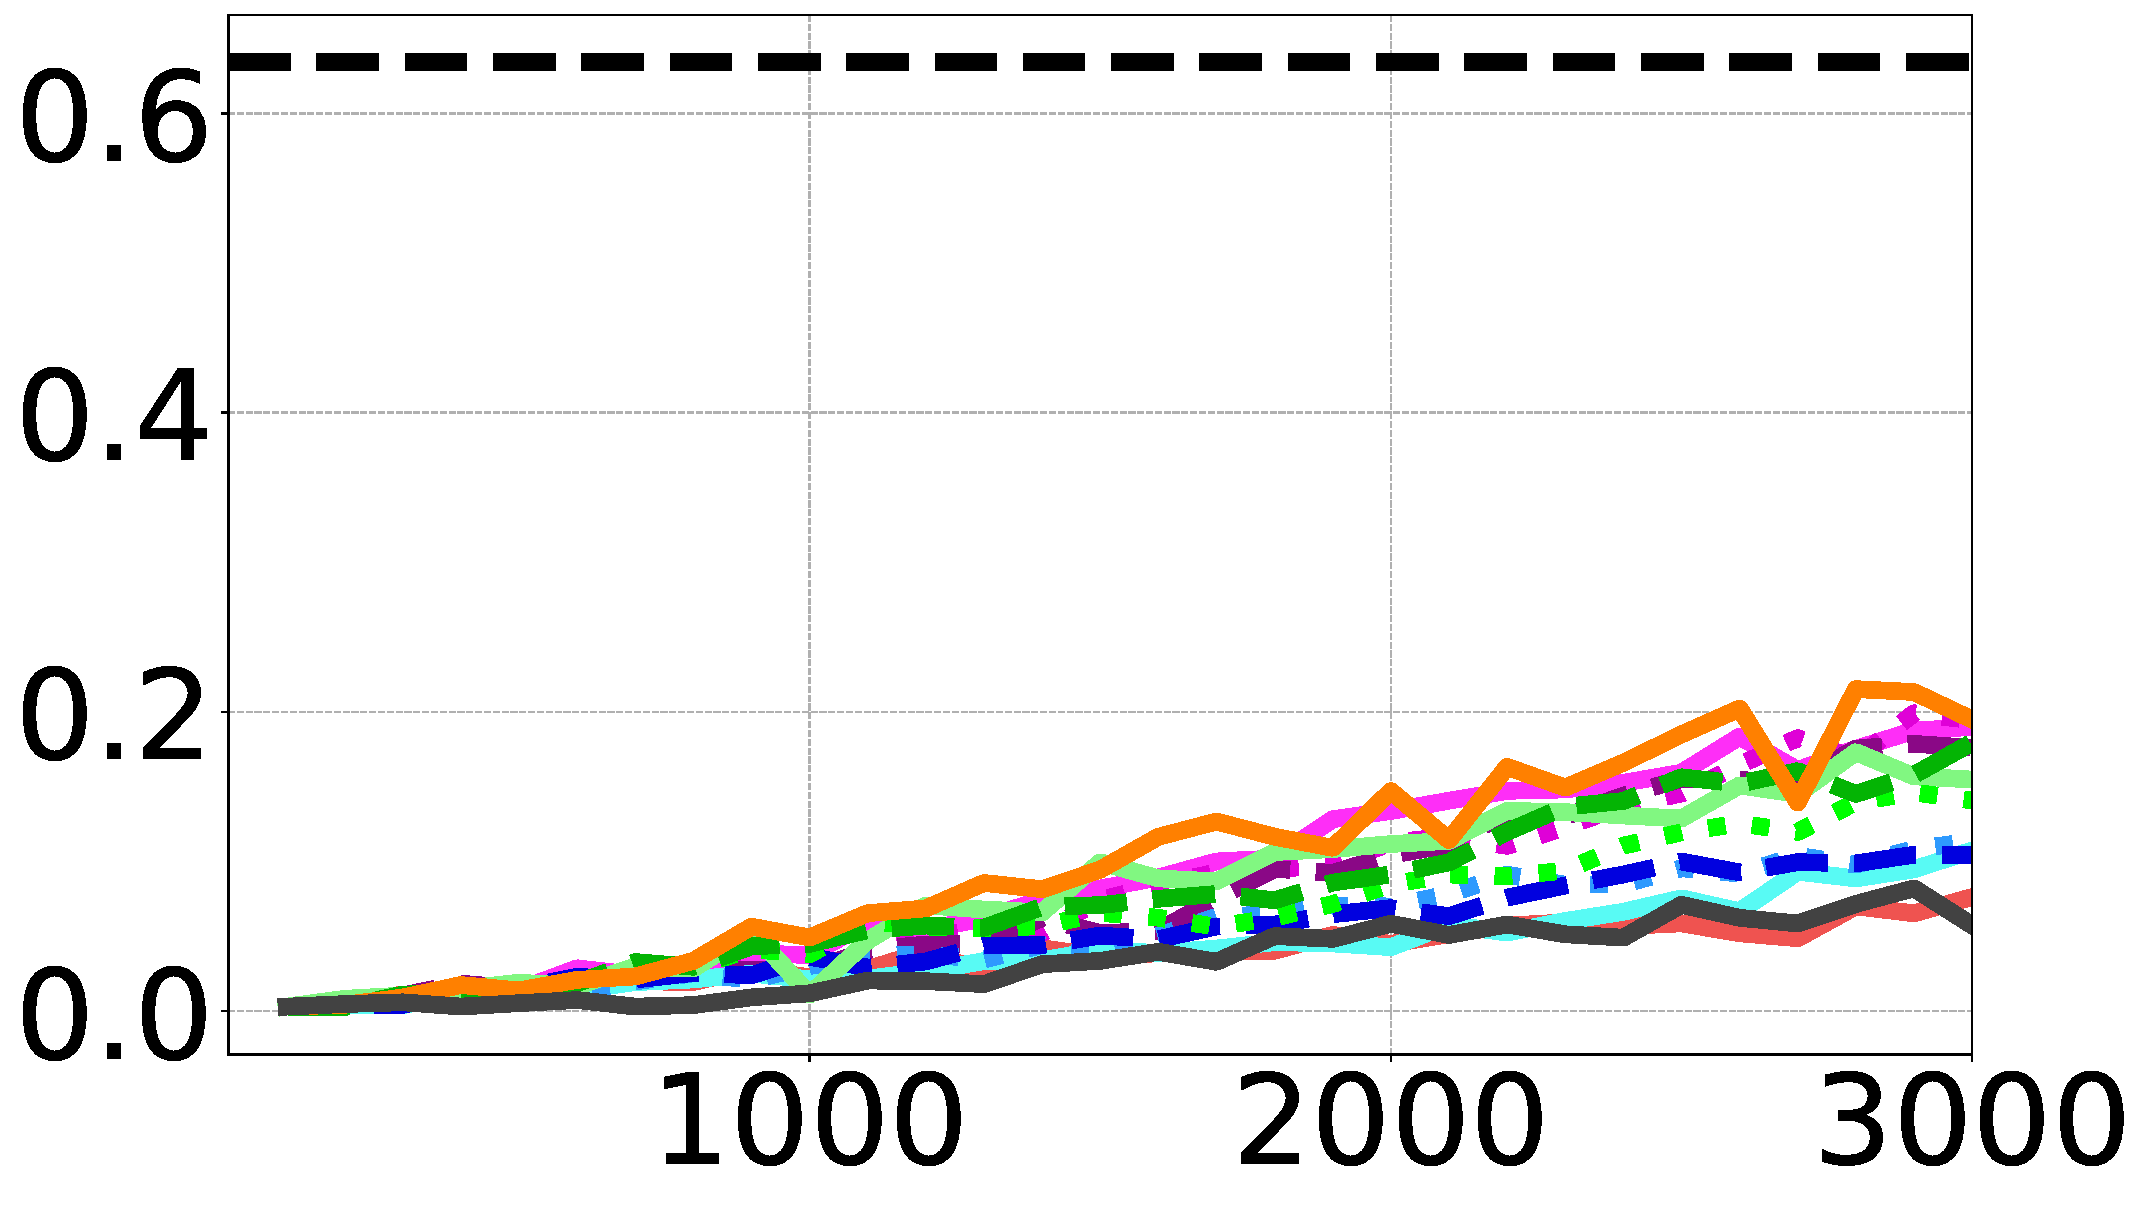
\includegraphics[width=0.24\textwidth]{figs/bert_yanjing_acc_all.pdf}}
	\end{center}

	\noindent
	\begin{center}
		\subfloat[Biomedical]{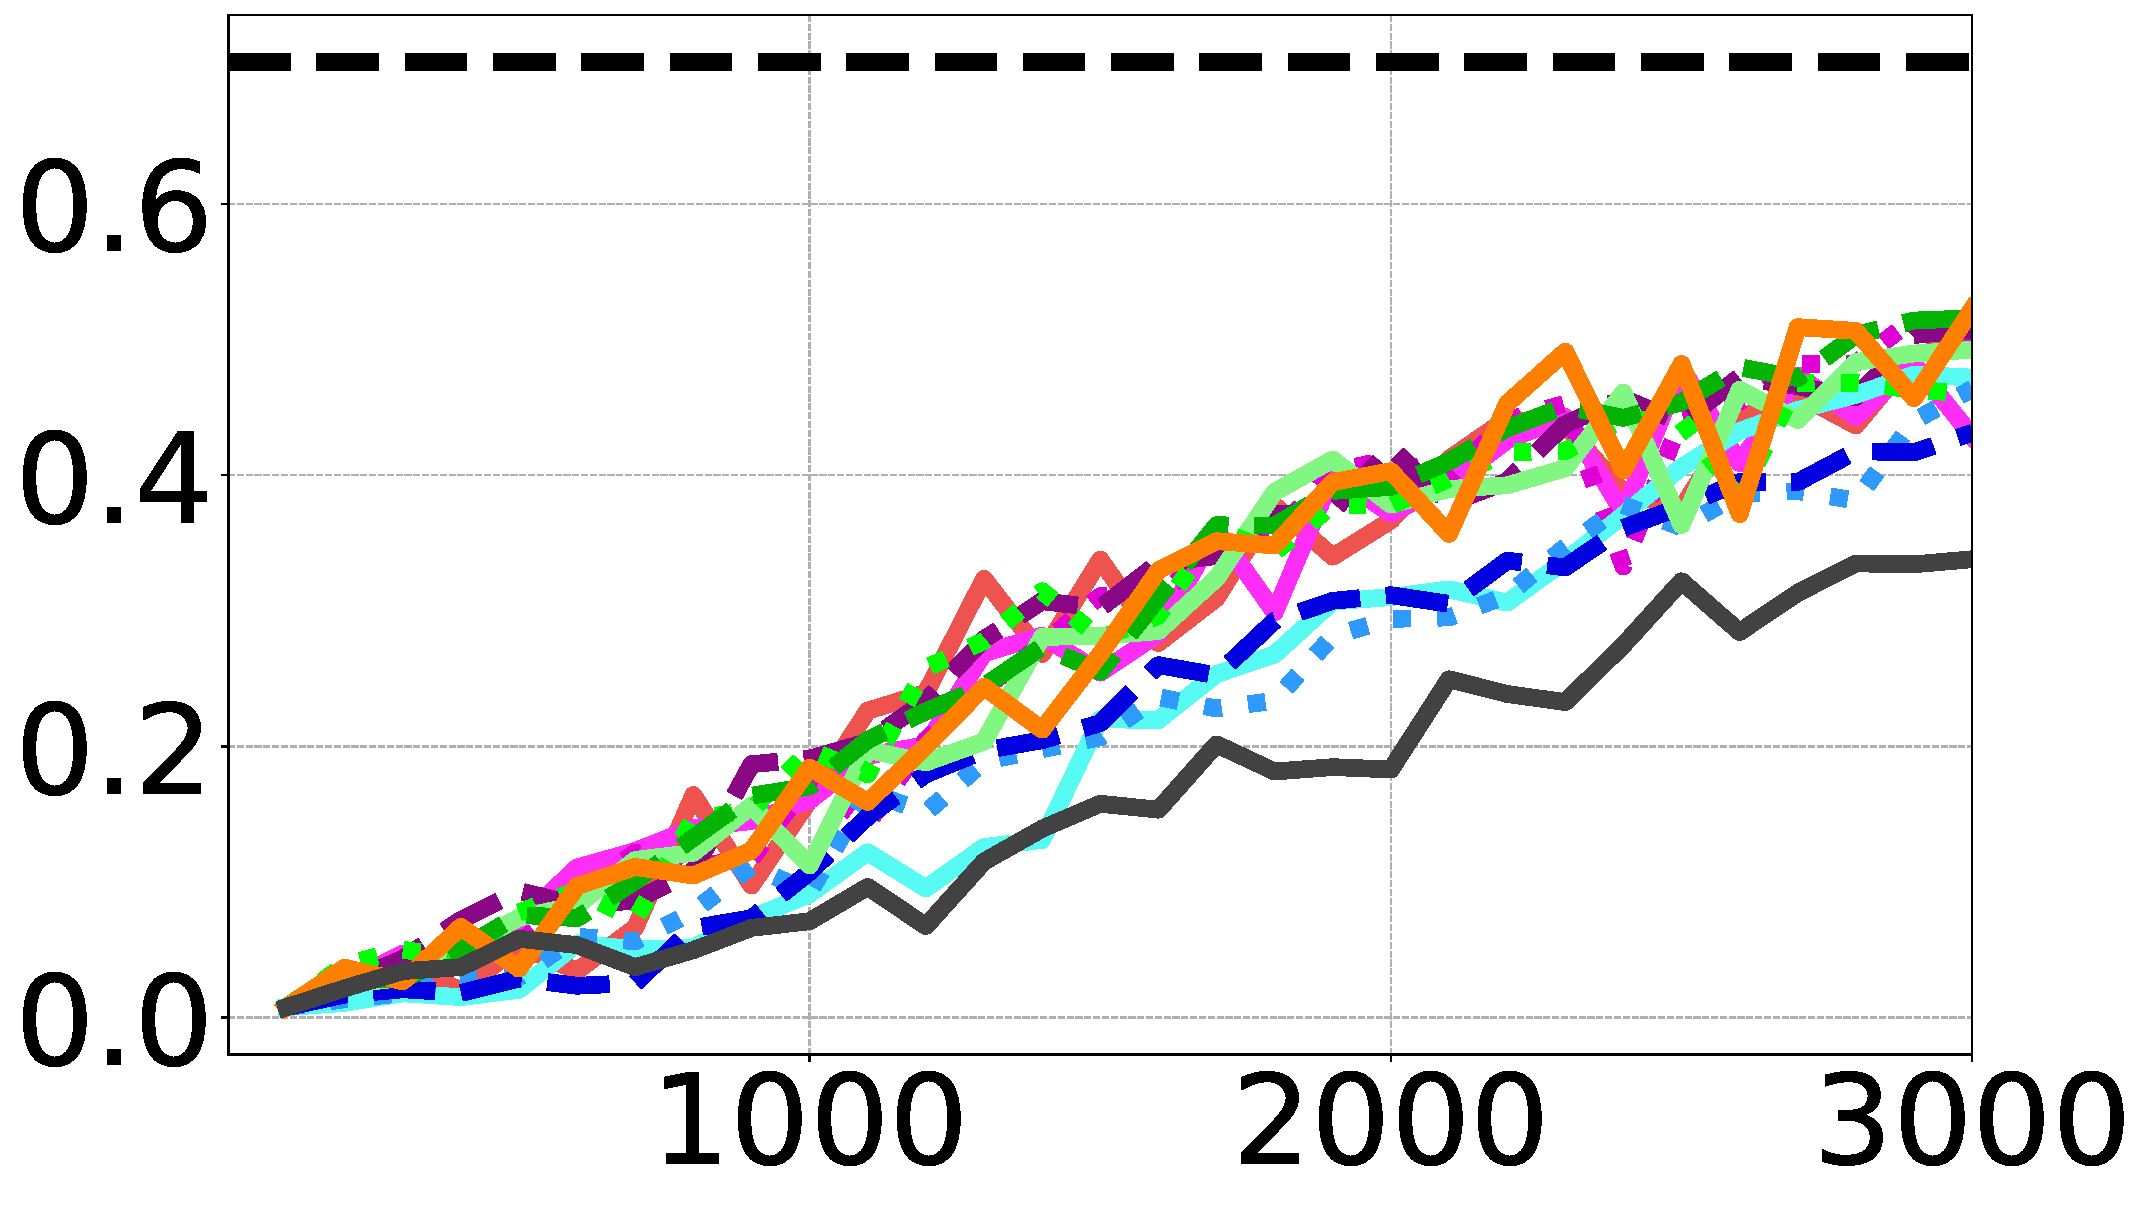
\includegraphics[width=0.24\textwidth]{figs/bert_Bio_acc_all.pdf}}
		\subfloat[StackOverflow]{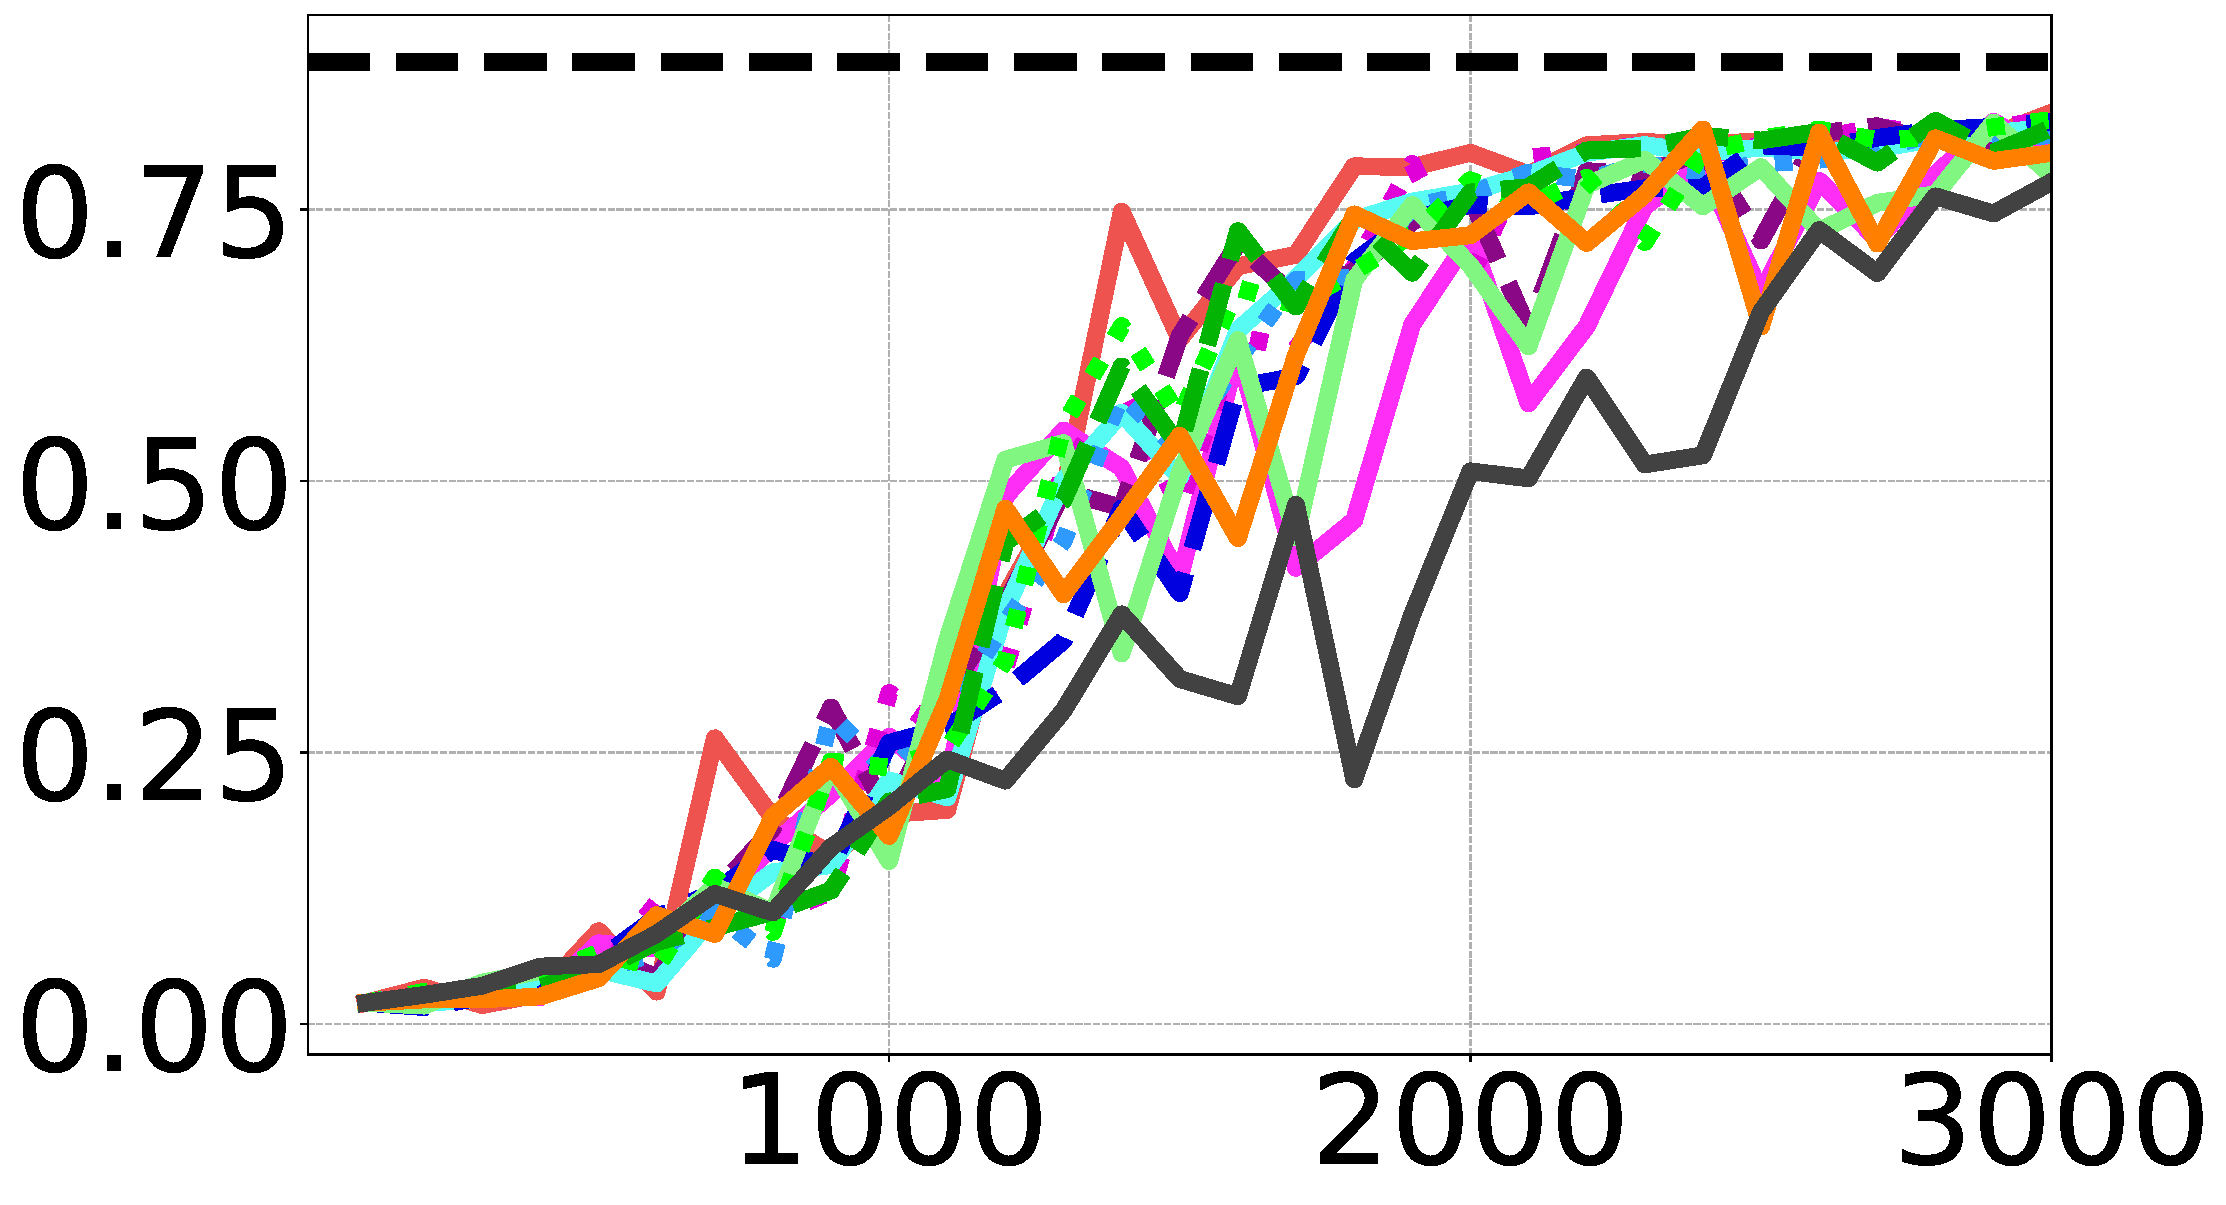
\includegraphics[width=0.24\textwidth]{figs/bert_SO_acc_all.pdf}}
	\end{center}
	\noindent
	\begin{center}
		\subfloat[SearchSnippets]{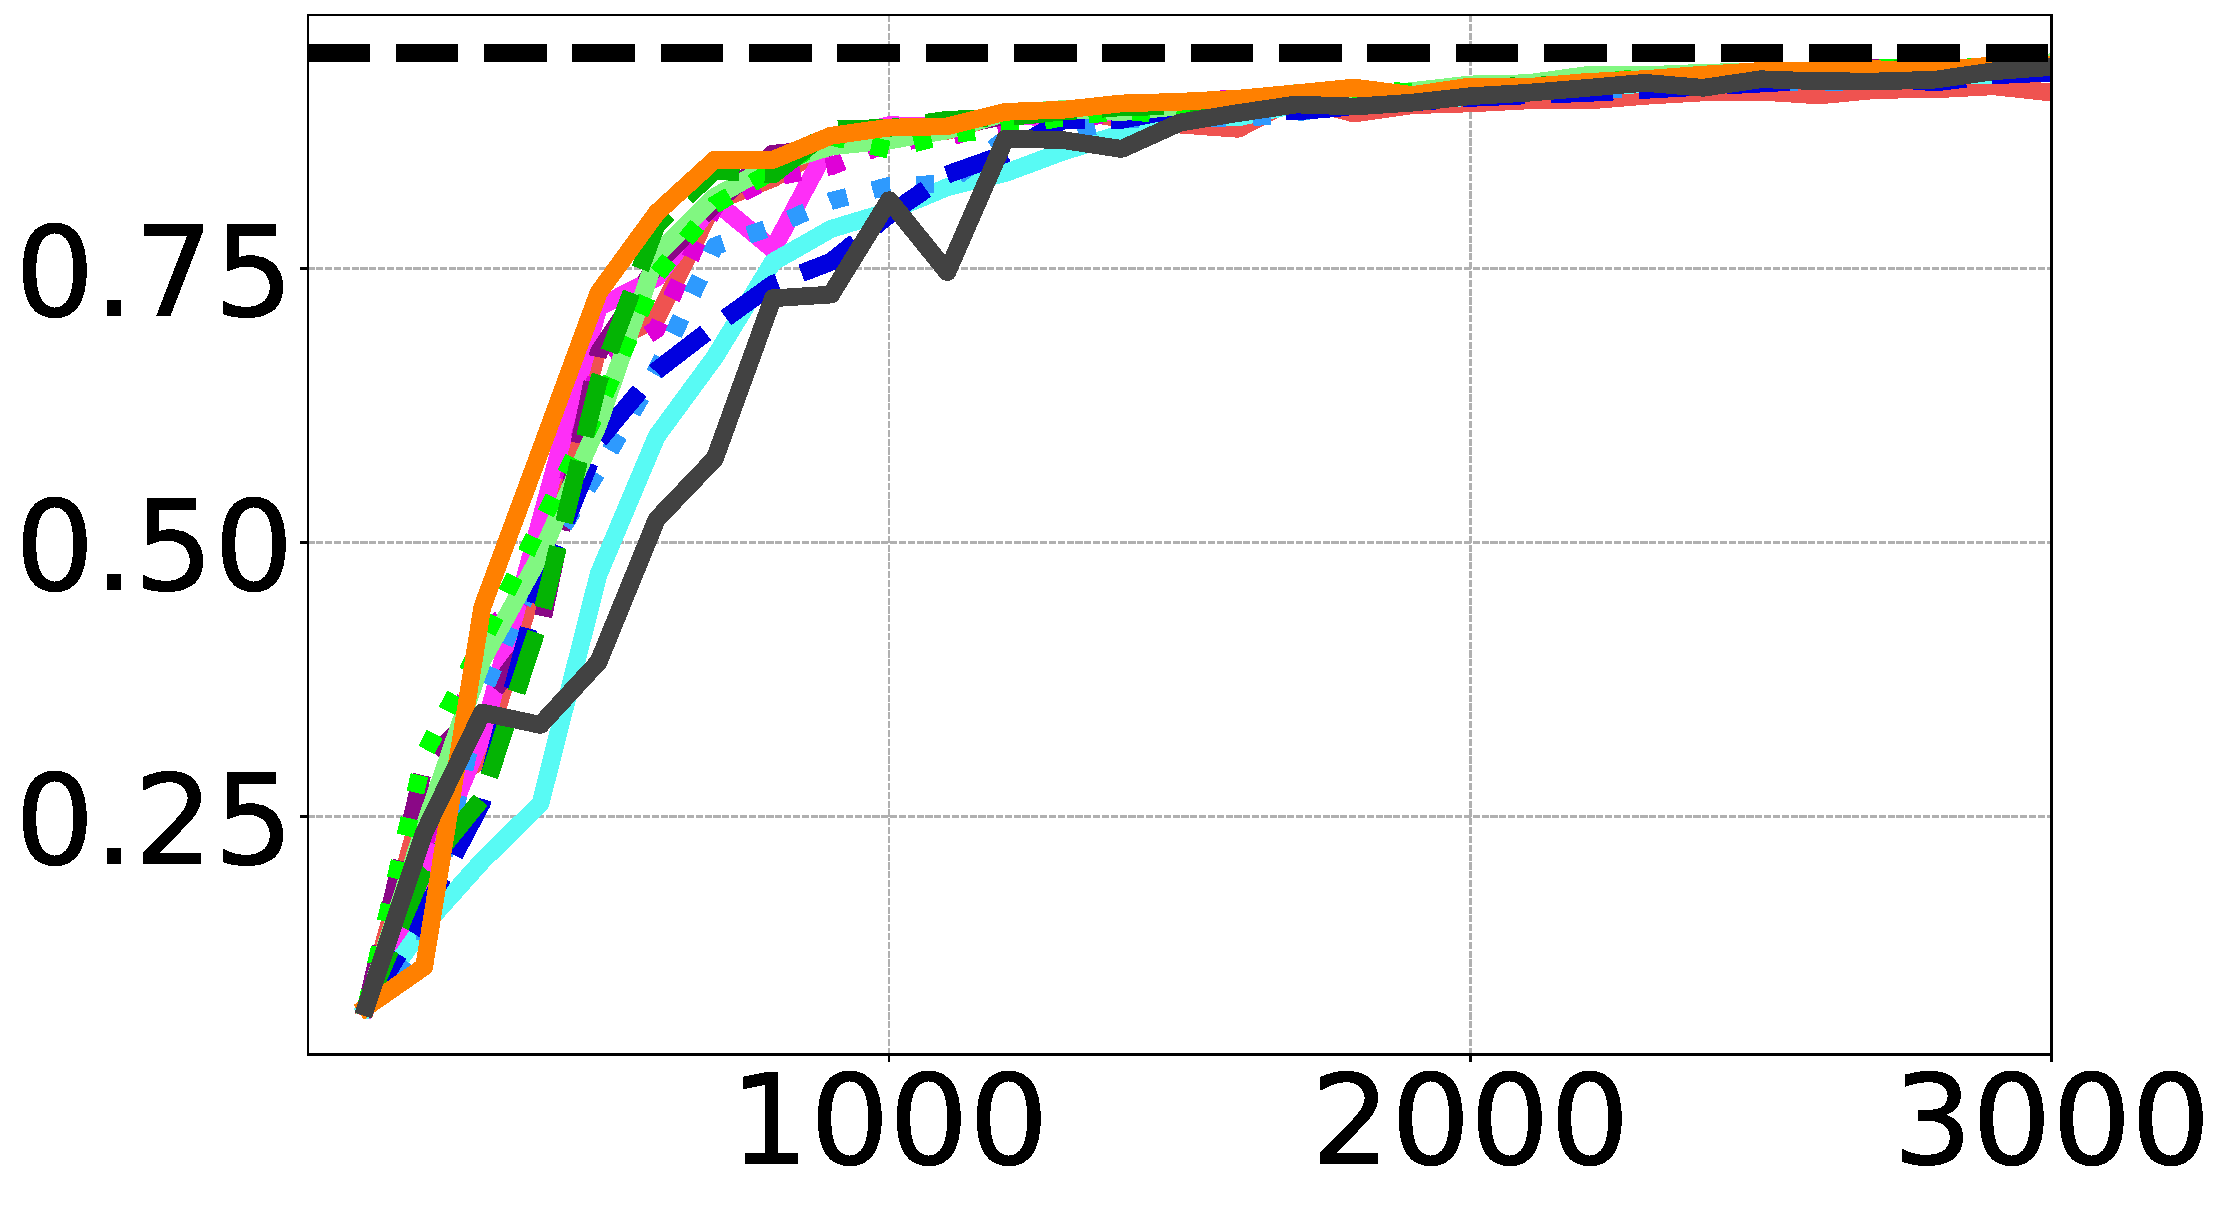
\includegraphics[width=0.24\textwidth]{figs/bert_Search_acc_all.pdf}}
	\end{center}

	\caption{Macro F1 curve of AL approaches on 8 datasets using BERT}
	\label{fig:acc_all_bert}
\end{figure}

\begin{figure}[th!]%[!hbt]
	\noindent
	\begin{center}
		\subfloat[Reuters]{\includegraphics[width=0.24\textwidth]{figs/lstm_pytorch_reuters_new_acc_all.pdf}}
		\subfloat[HuffPost]{\includegraphics[width=0.24\textwidth]{figs/lstm_pytorch_news_tokenized_fixed_acc_all.pdf}}
	\end{center}
	\noindent
	\begin{center}
		\subfloat[TNEWS]{\includegraphics[width=0.24\textwidth]{figs/lstm_pytorch_tnews_tokenized_acc_all.pdf}} % \newline
		\subfloat[GCS]{\includegraphics[width=0.24\textwidth]{figs/lstm_pytorch_yanjing_tokenized_acc_all.pdf}}
	\end{center}
	\noindent
	\begin{center}
		\subfloat[Biomedical]{\includegraphics[width=0.24\textwidth]{figs/lstm_pytorch_Biomedical_tokenized_acc_all.pdf}}
		\subfloat[StackOverflow]{\includegraphics[width=0.24\textwidth]{figs/lstm_pytorch_SO_tokenized_acc_all.pdf}}
	\end{center}
	\noindent
	\begin{center}
		\subfloat[SearchSnippets]{\includegraphics[width=0.24\textwidth]{figs/lstm_pytorch_SearchSnippets_tokenized_acc_all.pdf}}
		\subfloat[Book]{\includegraphics[width=0.24\textwidth]{figs/lstm_pytorch_book_tokenized_fixed_acc_all.pdf}}
	\end{center}
	\caption{Macro F1 curve of AL approaches on 8 datasets using LSTM+ATTN}
	\label{fig:acc_all_lstm}
\end{figure}

\begin{figure}[th!]%[!hbt]
	\noindent
	\begin{center}
		\subfloat[Reuters]{\includegraphics[width=0.24\textwidth]{figs/cnn_pytorch_reuters_new_acc_all.pdf}}
		\subfloat[HuffPost]{\includegraphics[width=0.24\textwidth]{figs/cnn_pytorch_news_tokenized_acc_all.pdf}}
	\end{center}

	\noindent
	\begin{center}
		\subfloat[TNEWS]{\includegraphics[width=0.24\textwidth]{figs/cnn_pytorch_tnews_tokenized_acc_all.pdf}} % \newline
		\subfloat[GCS]{\includegraphics[width=0.24\textwidth]{figs/cnn_pytorch_yanjing_tokenized_acc_all.pdf}}
	\end{center}
	\begin{center}
		\subfloat[Biomedical]{\includegraphics[width=0.24\textwidth]{figs/cnn_pytorch_Biomedical_tokenized_acc_all.pdf}}
		\subfloat[StackOverflow]{\includegraphics[width=0.24\textwidth]{figs/cnn_pytorch_SO_tokenized_acc_all.pdf}}
	\end{center}
	\noindent
	\begin{center}
		\subfloat[SearchSnippets]{\includegraphics[width=0.24\textwidth]{figs/cnn_pytorch_SearchSnippets_tokenized_acc_all.pdf}}
		\subfloat[Book]{\includegraphics[width=0.24\textwidth]{figs/cnn_pytorch_book_tokenized_acc_all.pdf}}
	\end{center}
	\caption{Macro F1 curve of AL approaches on 8,,, datasets using CNN}
	\label{fig:acc_all_cnn}
\end{figure}



%\subsection{Other models}
%In order to compare the performance on different deep models, we have chosen CNN, LSTM with attention as well as BERT as classifier. \figref{fig:acc_all_bert} depicts the macro F1 on different datasets using BERT.

% \begin{figure*}
% 	\centering
% 	\subfloat[Legend]{\includegraphics[width=0.2\textwidth]{figs/legend.pdf}}
% 	\subfloat[Reuters]{\includegraphics[width=0.2\textwidth]{figs/reuters_acc_all.pdf}}
% 	\subfloat[SQD]{\includegraphics[width=0.2\textwidth]{figs/stackoverflow_acc_all.pdf}}
% 	\subfloat[TNEWS]{\includegraphics[width=0.2\textwidth]{figs/tnews_acc_all.pdf}}
% 	\subfloat[GCS]{\includegraphics[width=0.2\textwidth]{figs/yanjing_acc_all.pdf}}
% 	\caption{Macro-F1 score of all classes} 
% 	\label{fig:acc_all}
% \end{figure*}

% \begin{table*}[]
% 	\centering
% 	\small
% 	\begin{tabular}{ccccccccc}
% 		\toprule
% 		\multirow{2}{*}{Method} & \multicolumn{4}{c}{Reuters} & \multicolumn{4}{c}{SQD} \\
% 		\cmidrule(lr){2-5} \cmidrule(lr){6-9}
% 		& 2     & 5    & 10    & all    & 2    & 5    & 10    & all   \\ \hline
	
% Entropy & 1.36 & 13.09 & 64.58 & 148.56 & 1.85 & 1.22 & 0.69 & -3.82\\
% Entropy freq & 0.97 & 11.96 & 59.88 & 137.93 & 2.08 & 1.81 & -0.21 & -0.43\\
% Entropy sqrtfreq & 1.09 & 12.86 & 64.11 & 153.28 & 1.83 & 1.02 & -0.72 & 0.44\\ \hline
% Density & 0.93 & 10.38 & 46.98 & 97.94 & 1.93 & 1.17 & -1.63 & -6.84\\
% Density freq & 1.08 & 10.7 & 56.66 & 108.85 & 1.69 & 1.38 & -1.55 & -3.58\\
% Density sqrtfreq & 0.78 & 9.7 & 57.55 & 119.56 & 2.04 & 0.79 & -1.11 & -4.31\\ \hline
% Radius & 1.24 & 12.75 & 62.48 & 168.61 & 1.97 & 0.92 & -0.62 & -1.15\\
% Radius freq & 1.37 & 11.41 & 64.32 & 135.56 & 1.98 & 2.22 & 0.4 & 0.71\\
% Radius sqrtfreq & 1.34 & 12.82 & 64.1 & 140.35 & 1.98 & 1.27 & -0.11 & 0.73\\ \hline
% Active & 1.35 & 11.83 & 65.1 & 178.51 & 1.5 & 1.34 & -0.66 & -6.47\\
% Center & 1.52 & 12.3 & 59.76 & 130.25 & 0.87 & -0.83 & -1.95 & -1.78\\
% 		\hline
% 	\end{tabular}
% 	\caption{Improvement of Methods on English Datasets, 1000}
% 	\label{table:effectOfFreq_en}
% \end{table*}



% \begin{table*}[]
% 	\centering
% 	\small
% 	\begin{tabular}{ccccccccc}
% 		\toprule
% 		\multirow{2}{*}{Method} & \multicolumn{4}{c}{TNEWS} & \multicolumn{4}{c}{GCS} \\
% 		\cmidrule(lr){2-5} \cmidrule(lr){6-9}
% 		& 2     & 5    & 10    & all    & 2    & 5    & 10    & all   \\ \hline
% Entropy & 1.68 & 2.71 & 4.02 & -0.15 & 1.73 & 2.49 & 2.7 & 7.19\\
% Entropy freq & 1.16 & 2.52 & 4.2 & 0.17 & 2.09 & 2.64 & 3.76 & 13.13\\
% Entropy sqrtfreq & 1.27 & 2.65 & 4.29 & 0.55 & 1.53 & 2.48 & 3.62 & 10.9\\ \hline
% Density & 1.38 & 2.37 & 1.54 & -2.19 & 1.47 & 2.46 & 2.39 & 12.49\\
% Density freq & 1.11 & 0.69 & 2.0 & 1.17 & 1.49 & 2.34 & 2.79 & 15.51\\
% Density sqrtfreq & 1.0 & 1.35 & 1.43 & -0.95 & 1.54 & 2.32 & 2.13 & 13.15\\ \hline
% Radius & 1.46 & 3.23 & 5.11 & -0.14 & 1.49 & 2.48 & 2.05 & 6.83\\
% Radius freq & 1.49 & 1.85 & 3.18 & 0.12 & 1.65 & 2.1 & 2.21 & 16.5\\
% Radius sqrtfreq & 1.35 & 2.86 & 4.16 & -0.38 & 2.1 & 2.5 & 3.57 & 10.8\\ \hline
% Active & 0.88 & -0.35 & -3.77 & -7.08 & 1.76 & 2.43 & -1.47 & -5.95\\
% Center & 0.61 & -4.84 & -9.59 & -8.41 & 1.81 & 0.37 & -3.79 & 3.52\\

% 		\hline
% 	\end{tabular}
% 	\caption{Improvement of Methods on Chinese , 1000}
% 	\label{table:effectOfFreq_cn}
% \end{table*}


% \begin{table*}[]
% 	\centering
% 	\small
% 	\begin{tabular}{ccccccccc}
% 		\toprule
% 		\multirow{2}{*}{Method} & \multicolumn{4}{c}{Reuters} & \multicolumn{4}{c}{SQD} \\
% 		\cmidrule(lr){2-5} \cmidrule(lr){6-9}
% 		& 2     & 5    & 10    & all    & 2    & 5    & 10    & all   \\ \hline
		
% Entropy & 1.28 & 9.51 & 42.89 & 178.97 & 1.3 & 0.9 & 1.03 & -4.73\\
% Entropy freq & 1.04 & 8.39 & 40.93 & 174.54 & 1.48 & 1.53 & 0.25 & -0.49\\
% Entropy sqrtfreq & 1.16 & 9.37 & 42.45 & 184.59 & 1.44 & 1.04 & -0.04 & 0.11\\ \hline
% Density & 1.07 & 7.85 & 35.32 & 132.78 & 1.44 & 1.13 & -1.12 & -6.36\\
% Density freq & 1.15 & 8.16 & 39.32 & 135.57 & 1.25 & 1.58 & -0.65 & -3.46\\
% Density sqrtfreq & 0.85 & 7.57 & 39.28 & 149.74 & 1.59 & 0.93 & -0.52 & -4.61\\ \hline
% Radius & 1.32 & 9.27 & 42.32 & 194.79 & 1.42 & 0.7 & -0.09 & -3.5\\
% Radius freq & 1.37 & 8.34 & 42.73 & 175.81 & 1.45 & 1.9 & 0.6 & 0.69\\
% Radius sqrtfreq & 1.36 & 9.44 & 42.64 & 182.29 & 1.38 & 1.0 & 0.38 & -0.19\\ \hline
% Active & 1.38 & 8.92 & 43.47 & 203.13 & 1.18 & 1.12 & 0.49 & -6.45\\
% Center & 1.46 & 9.16 & 40.19 & 131.81 & 0.57 & -0.3 & -0.77 & -1.02\\

% 		\hline
% 	\end{tabular}
% 	\caption{Improvement of Methods on English Datasets, 2000}
% 	\label{table:effectOfFreq_en}
% \end{table*}



% \begin{table*}[]
% 	\centering
% 	\small
% 	\begin{tabular}{ccccccccc}
% 		\toprule
% 		\multirow{2}{*}{Method} & \multicolumn{4}{c}{TNEWS} & \multicolumn{4}{c}{GCS} \\
% 		\cmidrule(lr){2-5} \cmidrule(lr){6-9}
% 		& 2     & 5    & 10    & all    & 2    & 5    & 10    & all   \\ \hline
% 		Entropy & 1.99 & 2.96 & 4.05 & 0.75 & 2.83 & 2.54 & 3.74 & 8.83\\
% 		Entropy freq & 1.85 & 2.97 & 4.67 & 1.84 & 2.9 & 2.59 & 4.52 & 18.54\\
% 		Entropy sqrtfreq & 1.79 & 3.15 & 4.31 & 2.35 & 2.57 & 2.47 & 4.31 & 16.05\\ \hline
% 		Density & 1.87 & 2.52 & 2.66 & -1.33 & 2.41 & 2.46 & 3.25 & 15.77\\
% 		Density freq & 1.73 & 1.73 & 2.55 & 2.0 & 2.56 & 2.35 & 3.37 & 20.53\\
% 		Density sqrtfreq & 1.65 & 2.05 & 2.2 & 0.25 & 2.52 & 2.31 & 3.01 & 18.41\\ \hline
% 		Radius & 1.9 & 3.19 & 4.72 & 0.94 & 2.54 & 2.58 & 3.23 & 9.43\\
% 		Radius freq & 2.0 & 2.48 & 3.93 & 1.86 & 2.73 & 2.31 & 3.18 & 19.52\\
% 		Radius sqrtfreq & 1.92 & 3.1 & 4.67 & 1.99 & 2.94 & 2.63 & 3.81 & 16.79\\ \hline
% 		Active & 1.42 & 0.77 & -1.21 & -5.48 & 3.02 & 2.48 & 1.75 & -1.5\\
% 		Center & 1.17 & -2.4 & -6.35 & -7.89 & 2.96 & 0.57 & -1.31 & 3.08\\
		
% 		\hline
% 	\end{tabular}
% 	\caption{Improvement of Methods on Chinese , 2000}
% 	\label{table:effectOfFreq_cn}
% \end{table*}

% \begin{table*}[]
% 	\centering
% 	\small
% 	\begin{tabular}{ccccccccc}
% 		\toprule
% 		\multirow{2}{*}{Method} & \multicolumn{4}{c}{Reuters} & \multicolumn{4}{c}{SQD} \\
% 		\cmidrule(lr){2-5} \cmidrule(lr){6-9}
% 		& 2     & 5    & 10    & all    & 2    & 5    & 10    & all   \\ \hline
		
% 		Entropy & 1.06 & 7.56 & 29.31 & 161.6 & 0.78 & 1.19 & 1.05 & -4.32\\
% 		Entropy freq & 0.9 & 6.75 & 28.14 & 156.37 & 0.9 & 1.63 & 0.49 & -0.4\\
% 		Entropy sqrtfreq & 1.0 & 7.38 & 29.09 & 162.14 & 0.86 & 1.34 & 0.32 & -0.34\\ \hline
% 		Density & 0.94 & 6.41 & 24.78 & 130.73 & 0.95 & 1.26 & -0.66 & -5.75\\
% 		Density freq & 1.04 & 6.6 & 27.32 & 131.84 & 0.83 & 1.71 & -0.03 & -3.18\\
% 		Density sqrtfreq & 0.83 & 6.29 & 27.15 & 144.01 & 1.03 & 1.29 & -0.16 & -4.28\\ \hline
% 		Radius & 1.11 & 7.28 & 29.1 & 170.41 & 0.86 & 1.03 & 0.28 & -3.64\\
% 		Radius freq & 1.13 & 6.71 & 29.3 & 158.71 & 0.88 & 1.92 & 0.83 & 0.45\\
% 		Radius sqrtfreq & 1.13 & 7.39 & 29.23 & 163.08 & 0.82 & 1.22 & 0.62 & -0.46\\ \hline
% 		Active & 1.13 & 7.12 & 29.77 & 174.2 & 0.71 & 1.5 & 0.8 & -5.66\\
% 		Center & 1.19 & 7.24 & 27.17 & 107.97 & 0.18 & -0.12 & 0.13 & -0.69\\
		
% 		\hline
% 	\end{tabular}
% 	\caption{Improvement of Methods on English Datasets, 3000}
% 	\label{table:effectOfFreq_en}
% \end{table*}



% \begin{table*}[]
% 	\centering
% 	\small
% 	\begin{tabular}{ccccccccc}
% 		\toprule
% 		\multirow{2}{*}{Method} & \multicolumn{4}{c}{TNEWS} & \multicolumn{4}{c}{GCS} \\
% 		\cmidrule(lr){2-5} \cmidrule(lr){6-9}
% 		& 2     & 5    & 10    & all    & 2    & 5    & 10    & all   \\ \hline
% 		Entropy & 1.95 & 3.0 & 3.98 & 1.23 & 3.14 & 2.66 & 4.05 & 9.96\\
% 		Entropy freq & 1.85 & 3.04 & 4.69 & 2.78 & 3.15 & 2.68 & 4.68 & 19.96\\
% 		Entropy sqrtfreq & 1.82 & 3.16 & 4.21 & 3.01 & 2.96 & 2.57 & 4.56 & 18.12\\ \hline
% 		Density & 1.84 & 2.6 & 2.8 & -0.09 & 2.83 & 2.5 & 3.72 & 17.25\\
% 		Density freq & 1.74 & 2.09 & 2.64 & 2.21 & 2.89 & 2.41 & 3.79 & 21.88\\
% 		Density sqrtfreq & 1.7 & 2.28 & 2.6 & 1.65 & 2.92 & 2.45 & 3.38 & 19.37\\ \hline
% 		Radius & 1.86 & 3.19 & 4.53 & 1.55 & 2.98 & 2.66 & 3.74 & 10.59\\
% 		Radius freq & 1.95 & 2.65 & 4.08 & 2.61 & 3.15 & 2.47 & 3.74 & 20.37\\
% 		Radius sqrtfreq & 1.91 & 3.1 & 4.51 & 2.79 & 3.22 & 2.76 & 4.16 & 18.35\\ \hline
% 		Active & 1.48 & 1.1 & -0.41 & -4.55 & 3.33 & 2.59 & 2.94 & 0.93\\
% 		Center & 1.22 & -1.28 & -4.66 & -7.05 & 3.31 & 0.9 & -0.07 & 1.02\\
		
% 		\hline
% 	\end{tabular}
% 	\caption{Improvement of Methods on Chinese , 3000}
% 	\label{table:effectOfFreq_cn}
% \end{table*}


% \begin{table}[]
% 	\centering
% 	\small
% 	\begin{tabular}{lllll}
% 		\toprule
% 		Method           & 2 & 5 & 10 & all \\ \hline
% 		Random & 0.33 & 0.36 & 0.62 & 0.62 \\
% 		Active & 0.7 & 0.63 & 1.32 & 1.27 \\
% 		Center & 1.52 & 0.46 & 0.37 & 0.45 \\ \hline
% 		Density & 0.61 & 0.58 & 0.47 & 0.47 \\
% 		Density freq & 0.47 & 0.68 & 0.59 & 1.73 \\
% 		Density sqrtfreq & 0.84 & 0.43 & 0.46 & 0.66 \\ \hline
% 		Entropy & 1.68 & 1.83 & 1.9 & 0.63 \\
% 		Entropy freq & \textbf{1.75} & \textbf{1.87} & \textbf{1.68} & 0.95 \\
% 		Entropy sqrtfreq & 0.56 & 1.07 & 1.38 & 1.33 \\ \hline
% 		Radius & 0.8 & 1.61 & 1.44 & 0.94 \\
% 		Radius freq & 1.5 & 1.37 & 1.14 & \textbf{1.89} \\
% 		Radius sqrtfreq & 1.65 & 1.53 & 1.03 & 1.47 \\

% 		\bottomrule
% 	\end{tabular}
% \caption{MRR Score of all classes summed over datasets, 1000}
% \label{table:score_1000}
% \end{table}

% \begin{table}[]
% 	\centering
% 	\small
% 	\begin{tabular}{lllll}
% 		\toprule
% 		Method           & 2 & 5 & 10 & all \\ \hline
% 		Random & 0.33 & 0.35 & 0.44 & 0.62 \\
% 		Active & 1.7 & 0.67 & 1.52 & 1.26 \\
% 		Center & 1.68 & 0.46 & 0.38 & 0.44 \\ \hline
% 		Density & 0.65 & 0.66 & 0.48 & 0.43 \\
% 		Density freq & 0.49 & 0.85 & 0.54 & 1.75 \\
% 		Density sqrtfreq & 1.3 & 0.44 & 0.43 & 0.61 \\ \hline
% 		Entropy & 0.99 & 1.56 & \textbf{1.95} & 0.55 \\
% 		Entropy freq & 1.02 & 1.23 & 1.84 & 0.88 \\
% 		Entropy sqrtfreq & 0.63 & 1.17 & 1.09 & \textbf{2.0} \\ \hline
% 		Radius & 0.73 & 1.68 & 1.43 & 0.92 \\
% 		Radius freq & \textbf{1.83} & 1.38 & 1.12 & 1.92 \\
% 		Radius sqrtfreq & 1.06 & \textbf{1.98} & 1.17 & 1.03 \\
		
% 		\bottomrule
% 	\end{tabular}
% \caption{MRR Score of all classes summed over datasets, 2000}
% \label{table:score_2000}
% \end{table}

% \begin{table}[]
% 	\centering
% 	\small
% 	\begin{tabular}{lllll}
% 		\toprule
% 		Method           & 2 & 5 & 10 & all \\ \hline
% 		Random & 0.33 & 0.35 & 0.39 & 0.78 \\
% 		Active & \textbf{1.7} & 0.72 & 1.52 & 1.27 \\
% 		Center & 1.68 & 0.46 & 0.4 & 0.44 \\ \hline
% 		Density & 0.87 & 0.53 & 0.44 & 0.43 \\
% 		Density freq & 0.51 & 0.82 & 0.55 & 1.45 \\
% 		Density sqrtfreq & 1.31 & 0.49 & 0.41 & 0.65 \\ \hline
% 		Entropy & 1.44 & 1.56 & 1.92 & 0.54 \\
% 		Entropy freq & 0.83 & 1.23 & \textbf{2.34} & 1.06 \\
% 		Entropy sqrtfreq & 0.59 & 1.2 & 1.08 & 1.75 \\ \hline
% 		Radius & 0.76 & 1.68 & 1.01 & 0.89 \\
% 		Radius freq & 1.25 & 1.42 & 1.18 & \textbf{1.92} \\
% 		Radius sqrtfreq & 1.12 & \textbf{1.96} & 1.17 & 1.23 \\
		
% 		\bottomrule
% 	\end{tabular}
% \caption{MRR Score of all classes summed over datasets, 3000}
% \label{table:score_3000}
% \end{table}




